
\documentclass[12pt,twoside]{reedthesis}

\usepackage{graphicx,latexsym}
\usepackage{amssymb,amsthm,amsmath}
\usepackage{longtable,booktabs,setspace}
\usepackage[hyphens]{url}
\usepackage{tikz}
\usepackage{enumitem}

\usetikzlibrary{shapes,arrows}
\usetikzlibrary{calc}
\usepackage{rotating}
\usepackage{natbib}
\usepackage{hyperref}
\usepackage{epigraph}
\newtheorem*{remark}{Remark}
\newtheorem{definition}{Definition}
\newtheorem{lemma}{Lemma}
\newtheorem{theorem}{Theorem}
\newtheorem{conjecture}{Conjecture}
\newtheorem{corollary}{Corollary}
\newcommand{\Enc}{{\sf Enc}}
\newcommand{\Dec}{{\sf Dec}}
\newcommand{\Adv}{\sf Adv}
\newcommand{\Eval}{{\sf Eval}}
\newcommand{\E}{\mathcal{E}}
\newcommand{\N}{\mathbb{N}}
\newcommand{\A}{\mathcal{A}}
\newcommand{\R}{\mathbb{R}}
\newcommand{\Z}{\mathbb{Z}}
\newcommand{\B}{\textbf{B}}
\newcommand{\Hb}{\textbf{H}}
\newcommand{\inv}{^{-1}}
\newcommand{\LWE}{LWE}
\newcommand{\RLWE}{RLWE}
\newcommand{\DLWE}{DLWE}

\renewcommand{\vec}[1]{\mathbf{#1}}
\newcount\colveccount
\newcommand*\colvec[1]{
        \global\colveccount#1
        \begin{pmatrix}
        \colvecnext
}
\def\colvecnext#1{
        #1
        \global\advance\colveccount-1
        \ifnum\colveccount>0
                \\
                \expandafter\colvecnext
        \else
                \end{pmatrix}
        \fi
}
\tikzstyle{line} = [draw, -latex']

\title{Fully Homomorphic Encryption}
\author{Joshua Gancher}
\date{May 2016}
\division{Mathematics and Natural Sciences}
\advisor{Adam Groce}

\department{Mathematics}

\setlength{\parskip}{0pt}

\begin{document}

  \maketitle
  \frontmatter
  \pagestyle{empty}

 \chapter*{Acknowledgements}
 I owe many thanks to my advisor, Adam Groce, for all of the invaluable academic guidance and advice he has given me over the past year. I would like to also thank Jim Fix and Jerry Shurman for the insights they have given me during my time at Reed.

 I would like to thank my friends and colleagues, who have supported me throughout the thesis process. Among others, I'd like to acknowledge Haley, Philip, Hannah, Orla, Max, and Sarah for their \emph{distinguished} compatriotism.

 I would \textbf{not} like to thank Mick, who did nothing but distract me with sophistry and crises of form throughout the whole ordeal.

 Finally, I thank my parents, Susan and Stephen Gancher, without whom none of this would have been possible.


%\chapter*{Preface}
	Meum thesis est divisa in omnis tres.


\tableofcontents
%\listoftables
%\listoffigures


\chapter*{Abstract}
	\emph{Fully homomorphic encryption} (FHE) enables one to carry out computations using ciphertexts, rather than plaintexts. One may wish to compute the output of a boolean circuit $C$ given input bits $\{b_i\}$, in order to produce an output bit $b'$. With FHE, instead one can \emph{encrypt} each $b_i$ to create a ciphertext $c_i$, and run a corresponding computation ${\sf Eval}(C, \{c_i\})$ on the ciphertexts, in order to produce an output ciphertext $c'$. Then, one can decrypt $c'$ to retrieve $b'$.

    Crucially, a third party may run ${\sf Eval}$ using only the public key. By the security of the encryption scheme, this third party can run ${\sf Eval}$ to produce $c'$ out of the $c_i$, but not learn anything about $c'$ or any of the $c_i$ in the process. Only with the secret key can anybody learn about the contents of the ciphertexts.
    Using this technology, one may offload an arbitrary computation to somebody else without disclosing the contents of the data. Because of this, FHE is a highly applicable primitive. How to achieve FHE was a major open question until Craig Gentry's breakthrough 2009 thesis, which has since inspired years of cryptographic research.

    In this thesis, I survey this research. After outlining the relevant security definitions and hardness assumptions for FHE, I will present four major constructions of FHE schemes: Gentry's initial construction \cite{gentry2009fully}, the DGHV scheme over the integers \cite{dghv}, and two FHE schemes based off of the learning with errors problem \cite{bgv2011} \cite{gsw}. Afterwards, I will outline some applications of FHE.


%\input{tex/dedication}

\mainmatter
\pagestyle{fancyplain}

%---INTRODUCTION---
\chapter*{Introduction}
\addcontentsline{toc}{chapter}{Introduction}
\chaptermark{Introduction}
\markboth{Introduction}{Introduction}

Cryptography is, in part, the study of providing security guarantees on information. There are many such guarantees, but we will be most concerned with that of \emph{secrecy}. When we say secrecy, what we mean is this: two parties, Alice and Bob, are communicating with each other over an insecure channel (such as the Internet), where they want to keep their communications secret from a third party, Eve.

%what's encryption
Many situations fit this model. One classic example is that Alice and Bob are agents of a military who are trying to give each other crucial strategic information, such as commands to a troop. Then, Eve is a member of the opposing military, who would very much like to learn where Alice and Bob's soldiers are moving. Another example is communicating with one's bank, where Alice is a customer of bank Bob, and Eve is maliciously listening in on Alice's communication to the bank. There are two basic goals to be achieved in this model: the first is that Alice and Bob can understand what each other is saying, and the second is that Eve cannot learn what their messages contain.

Generally, the way to achieve these two goals is through \emph{encryption}. Encryption is a process that, when given a \emph{key} ${\sf K}_E$, converts \emph{plaintexts} (i.e., messages) to \emph{ciphertexts}. Instead of Alice and Bob communicating directly in plaintext, they instead encrypt their messages and send the ciphertext. Then, the recipient will \emph{decrypt} the ciphertext using the secret key ${\sf K}_D$, to reveal the original message. (The keys ${\sf K}_E$ and ${\sf K}_D$ are generated together ahead of time.)

Encryption is constrained to meet the two above goals:
\begin{enumerate}
    \item Encryption is \emph{correct}: if Alice encrypts a message using ${\sf K}_E$, then Bob can retrieve the correct message by decrypting the ciphertext with ${\sf K}_D$.
    \item Encryption is \emph{secure}: if Alice encrypts a message using ${\sf K}_E$, then Eve cannot use the ciphertext to learn about the underlying message without access to ${\sf K}_D$.
\end{enumerate}

When many people think about encryption, they think of the Enigma machine or similar World War II-era systems. These systems are called \emph{ciphers}, and are \emph{symmetric} in nature: that is, the key for encryption, ${\sf K}_E$, is the same as the key for decryption, ${\sf K}_D$. In this setting, Alice and Bob both possess this shared key ${\sf K}$, so can both decrypt each other's ciphertexts. A more modern example of a cipher is AES (Advanced Encryption Standard), which is used throughout the Internet for secure communication.


The other possibility, which is the one we are concerned with, is the \emph{asymmetric} setting (also called the \emph{public-key} setting). Here, the encryption key (the \emph{public key}) ${\sf K}_E$ is different than the decryption key (or the \emph{secret key}) ${\sf K}_D$. In this setting, Bob publishes his public key ${\sf K}_E$ so that anybody can see it, but only he possesses the secret key ${\sf K}_D$. This is a very useful technique, since Alice is now able to securely send messages to Bob \emph{using only public information}. That is, Alice may speak privately to Bob without Alice and Bob agreeing to be spoken to in advance, since only Bob possesses ${\sf K}_D$. Compare this with the symmetric key setting, in which Alice and Bob need to agree on the secret key ${\sf K}$ beforehand.

One of the first major public-key encryption system was invented by Rivest, Shamir, and Adleman in 1977 \cite{rivest1978method}, now named the RSA scheme. Following their discovery, Rivest and others became interested in not only what was possible using public-key encryption alone, but also what \emph{else} was possible using the same mathematical techniques as is used in RSA and other contemporary public-key encryption systems.

The reason they conjectured that more was possible using public-key encryption is that ciphertexts encrypted under RSA somehow contained ``more structure'' than ciphertexts encrypted under symmetric-key ciphers. Generally, ciphers regard messages as \emph{collections of bits}; that is, many individual choices of $1$s or $0$s. Then, the goal of a cipher is to ``mix up'' these bits, and ``add in'' new bits, so that the output of the cipher looks random -- subject to the constraint that we can reverse all of the operations taken by the cipher, given the key. In contrast, RSA regards messages as \emph{integers}, and performs arithmetic operations on these integers so that the integer output of RSA looks random -- subject to the corresponding constraint that we can reverse all of the arithmetic operations taken by RSA, given the secret key.

Because RSA operates on integers instead of individual bits, it might make sense to \emph{operate arithmetically on ciphertexts}. That is, since each ciphertext of RSA is itself an integer, it may make sense to add or multiply integers, where it would not make sense to add or multiply individual bits. It is in this sense that RSA contains more structure than symmetric-key ciphers.

Abstracted out from RSA, we search for an operation on public-key ciphertexts in which an ``outside'' operation -- computed on the ciphertext -- corresponds in some way to an ``inside'' operation -- a computation on the \emph{plaintexts}. A sufficiently powerful system of this sort would be extremely useful, since in effect we would be \emph{computing on ciphertexts}. That is, given some program $P$ with data $x$ ($x$ could be some sensitive medical information, and $P$ some computation involving medical data), we could transform $x$ into a ciphertext $c$, and run $P$ on $c$ instead.

It turns out that, when computing with integers, ``sufficiently powerful'' means that it makes sense to both add and multiply ciphertexts. However, all ``classic'' public key encryption systems (such as RSA) are \emph{not} sufficiently powerful. For example, it turns out that it \emph{does} make sense to multiply RSA ciphertexts -- and indeed, we receive a valid encryption of the messages multiplied together -- but it does not make sense to add ciphertexts. The same limitation holds for other public-key encryption systems similar to RSA. Thus, it has been a major open question within cryptography whether or not encryption systems exist that do have sufficiently powerful operations; that is, if they can support both addition and multiplication. Encryption systems with this capability are called \emph{homomorphic} encryption systems.

Homomorphic encryption has immediate applications to banking, science involving sensitive data (such as genomics), providing secrecy guarantees on programs as well as data, encrypted search queries, and so on. In medicine, for example, one could imagine that everyone's medical record is stored encrypted on a cloud service. Patients would submit their eating habits and exercise routine to this cloud service, also under a layer of encryption. Using homomorphic encryption, this cloud service could then automatically warn patients of health complications, bad eating habits, and so on -- all without the cloud service having access to the patient's medical data. Since the data is encrypted, such a system could enable hospitals to legally share encrypted medical records with the cloud service. Without homomorphic encryption, such a service could not exist.

This question was first raised by Rivest et al.~in 1978 \cite{rivest1978data}. More than thirty years later, Craig Gentry answered this question in the affirmative in 2009, giving an explicit construction of a \emph{fully homomorphic encryption} (FHE) scheme.

This thesis outlines his construction, and presents the academic work surrounding and extending his result from 2009 to the present day.


\section*{Outline of Thesis}
The thesis is divided into six main chapters. In Chapter 1, we give the relevant background for the definitions of encryption and FHE. In Chapter 2, we present the theory of \emph{lattices}, which are used by all FHE schemes in some manner. In Chapter 3, we present Gentry's FHE construction. In Chapter 4, we present the DGHV scheme, which is an FHE scheme defined over integers, constructed by van Dijk et al.~In Chapter 5, we present the most recent forms of FHE, which are based on the learning with errors (LWE) problem. Finally, in Chapter 6, we sketch some applications of FHE.



%---CHAPTERS---
\chapter{Background} \label{chap: background}
\section{Encryption}
	One of the most fundamental concepts in Cryptography is that of \textit{encryption}. To encrypt a message $m$ means that given an encryption key $\sf EK$, one can create an encryption $\Enc_{\sf EK}(m)$ such that without the decryption key $\sf DK$, no reasonable adversary can learn anything from the encryption. In the symmetric-key setting, $\sf EK = \sf DK$, and is deemed private knowledge. In the public key setting, $\sf EK$ is public, while $\sf DK$ is private. We will be concerned with the public key setting.

		Formally, a public key encryption scheme consists of the following three (probabilistic) algorithms:
	\begin{description}
	\item[KeyGen] takes as input a security parameter $\lambda$ and outputs a public encryption key $pk$ along with a secret decryption key $sk$.
	\item[Encrypt] takes as input a public key $pk$ and a message $m$, and outputs a ciphertext $c$.
	\item[Decrypt] takes as input a secret key $sk$ and a ciphertext $c$, and outputs a message $m$.
	\end{description}

	We abbreviate Encrypt$(pk, m)$ as $\Enc_{pk}(m)$, and similarly for Decrypt.

	Additionally, we require that decryption is correct; that is, given a pair of keys $pk, sk$ from KeyGen,
	\[\Dec_{sk}(\Enc_{pk}(m)) = m.\]


	We now need to make precise what we mean by ``reasonable adversary'', the ability to ``learn anything,'' and what it means that ``no reasonable adversary can'' learn something. By a ``reasonable adversary'', we mean a probabilistic algorithm whose running time is bounded by some polynomial of the \textit{security parameter}. A security parameter parametrizes how secure our desired encryption scheme is (usually at the cost of requiring more resources to execute, such as a longer key). By requiring that adversaries have running time polynomial in the security parameter, we assume that certain classes of attacks are infeasible, since they are conjectured to not have polynomial time implementations.

	This is formalized by a \emph{hardness assumption}, which asserts that some sort of computational problem is difficult for probabilistic polynomial time (PPT) algorithms. These formalizations do not refer to any specific cryptographic scheme, or the relevant security definition. Instead, the cryptographic scheme is proved secure relative to this formalization. If any algorithm can violate the security of the cryptographic scheme, then we can create an algorithm that breaks the hardness assumption. Thus, the cryptographic scheme is secure, since we assume no algorithm can break the hardness assumption. (This proof technique is called a \emph{reduction}.)

	We usually can't say that a PPT algorithm unequivocally \emph{cannot} solve some computational problem. Given any problem in NP, we can construct a PPT algorithm that randomly guesses the solution; with some small probability, this algorithm will be correct. If we assume the problem is sufficiently difficult, then the rate of success will be a \emph{negligible} function of the security parameter.

	\begin{definition} Let $f$ be a function from $\N$ to $\R$. Then $f$ is \emph{negligible} if it decays faster than the inverse of any polynomial; that is, for any polynomial $P$ such that $P(n) \geq 0$ for $n \in \N$, there exists an $N$ such that
	\[|f(n)| < \frac{1}{P(n)} \text{ for $n > N$.}\]
	\end{definition}

	For example, consider a computational problem that requires one to output a specific $n$-digit binary number. Suppose that the problem is so intractable that the best any PPT adversary can do is guess a number uniformly at random. Then, this adversary's probability of success is $\frac{1}{2^n}$, which is negligible. Relaxing this problem to one for which no polynomial time solution is known (such as integer factorization) keeps the probability of success negligible.

	There are several notions of what it means for a PPT adversary to learn anything from our encryption scheme. The notion that we will be concerned with is a \textit{game-based definition.}

\subsection{Game-based IND-CPA}

	The goal is to formalize what we mean by the adversary learning anything from some given encryption $\Enc_{\sf EK}(m)$. Abstracted from any use case, the correct wish is that \textit{the adversary cannot distinguish two encryptions of different messages from each other.} This captures all information-theoretic intuitions behind encryption: if the adversary could learn something substantial about $m$ from $\Enc(m)$, the adversary could distinguish this encryption from  $\Enc(m')$, where the relevant information in $m'$ is different than the information in $m$.

	To quantify the ability for a PPT adversary $\A$ to distinguish between two different encryptions, the following game is played between $\A$ and another party, called the \textit{challenger}:
	\begin{definition}[IND-CPA Game]
	\ \\
	\begin{enumerate}
	\item Given the security parameter $\lambda$, the challenger generates keys $pk, sk$ from {\sf KeyGen}. The security parameter $\lambda$ and the public key $pk$ is given to $\A$.
	\item The adversary $\A$ may perform some number of test encryptions $\Enc_{pk}(m)$, or any other computations. (The adversary is bounded in operations by some polynomial in $\lambda$.)
	\item The adversary outputs two messages $m_0, m_1$ to the challenger.
	\item The challenger uniformly selects a random bit $b \leftarrow \{0, 1\}.$ The challenger creates the encryption $c = \Enc_{pk}(m_b)$, and sends $c$ to the adversary. (This $c$ is called the \emph{challenge ciphertext}.)
	\item After some amount of final computation, $\A$ outputs a bit $b'$.
	\end{enumerate}
	\end{definition}

	The goal of this game is for $\A$ is to guess the secret bit $b$. The name IND-CPA stands for \textit{indistinguishability} under a \textit{chosen plaintext attack}. A chosen-plaintext attack means that $A$ is allowed to obtain encryptions $\Enc_{pk}(m)$ for any message $m$.

	Note that a trivial adversary who always guesses $b' = 1$ has a probability of winning $\frac{1}{2}$. A scheme is IND-CPA secure if no adversary can do any better.

	\begin{definition} An encryption scheme \textit{\sf KeyGen, \Enc, \Dec} is IND-CPA secure if for all PPT adversaries $\A$, there exists a negligible function $\varepsilon$ such that
	\[|\Pr[b = b'] - \frac{1}{2}| \leq \varepsilon(\lambda).\]
	\end{definition}

	Often, we will abbreviate the quantity $|\Pr[b = b'] - \frac{1}{2}|$ as \emph{the advantage of $\A$}, or $\Adv(\A)$.

	In the public key setting, the above definition is the weakest one worth considering. There exist stronger definitions of security, such as \textit{chosen ciphertext attacks}, where the adversary may also query $\Dec_{sk}(c^*)$ for $c^* \not = c$; however, this definition is outside of the current scope.

\section{Homomorphic Encryption} \label{sec:lkj}
While the above definition is satisfactory for many purposes, there are certain situations where we would like to do something more than just having encrypted data; we additionally want to \emph{use it}.

Suppose that a client is storing some large (encrypted) numerical database on a server, and that the client wishes to compute some statistical function of part of the database, such as a linear regression.

 In general, encryption schemes may be \emph{non-malleable}; that is, manipulating ciphertexts does not correspond to manipulating plaintexts in a usable way. If our encryption scheme is non-malleable, then there is only one way to compute our regression: we must download all of the data involved, and compute the regression ourselves. This may be highly undesirable, since we could be forced to download 500 GB of data to obtain a 2 KB result of computation.

 Instead, we search for a better way. We want ciphertexts that are malleable: that is, we wish for the server to compute our regression itself \emph{on the encrypted data}, and send us back only the 2 KB of regression data, still encrypted. (Of course, we wish for this encryption scheme to still be CPA secure. The server shouldn't be able to learn anything about the result of this computation.)

 Naturally, this brings up the issue of trusting the server. If the server is assumed to be adversarial with respect to learning about the ciphertexts, the server should also be assumed to be adversarial with respect to performing the correct computation on the ciphertexts. For the purpose of this thesis, however, we will assume that the server always performs the correct computation.


First, let us describe plaintext-side computation. Of course, what computations are available to us between two pieces of plaintext depends on what our set of possible plaintexts is; if our message space is $\{0,1\}^n$, more (2-ary) computations are available than if our message space is much smaller. Furthermore, how we interpret a message $m \in \{0,1\}^n$ changes what computations are available on those plaintexts; if we regard $m$ as an ordered collection of bits, then it makes sense to perform bitwise AND, exclusive or, etc. However, if we regard $m$ as some integer in the finite field $\mathbb{F}_q$, then it might make more sense to add and multiply messages.

The most simple situation we will consider is when $m$ is in $\{0, 1\}.$ Here, the relevant operations are the boolean operations: AND, OR, NAND, etc. Although this message space is much smaller, this does not limit our ability to compute; any desired computation can be written as a boolean circuit $C$, composed of logic gates. Equivalently, any desired computation can be expressed as a polynomial in $\mathbb{F}_2[x_1, \dots, x_n]$, where $n$ is the amount of binary inputs to the computation.

Now, suppose we have encryptions $\phi_0 = \Enc_{pk}$($b)$ and $\phi_1 = \Enc_{pk}$($b')$, where $b$ and $b'$ are in $\{0,1\}$. Ciphertext-side, we wish for an ability for the server, given only the public key, to compute $\phi^*$ such that $\Dec_{sk}(\phi^*)$ $= f(b, b')$, where $f$ is any chosen function from $\{0,1\} \times \{0,1\} \to \{0,1\}$. It suffices to be able to compute some functionally complete subset of operations; for example, given a way to compute $\phi^* = \textit{AND}(\phi_0, \phi_1)$ and $\phi^* = \textit{NOT}(\phi)$, any other function $f$ can be derived.

Thus, we obtain the first requirement for our new scheme: in addition to KeyGen, Encrypt, and Decrypt, we have an algorithm Evaluate (abbreviated $\Eval$) which takes as input the public key $pk$, a boolean circuit $C$, and a set of input ciphertexts $c_i = \Enc_{pk}(\pi_i)$, and outputs a new ciphertext $c'$ such that $\Dec_{sk}$$(c')$ is equal to $C(\pi_1, \dots, \pi_n)$.

While we eventually will want our encryption scheme $\mathcal{E}$ to be able to evaluate all circuits, our initial definition is quantified over a certain set of \emph{permissible} circuits, notated $\mathcal{C}_\mathcal{E}$.


\begin{definition} (Correct evaluation, adapted from \cite{gentry2009fully})
An encryption scheme $\E$ \emph{correctly evaluates} a circuit family $\mathcal{C}_\mathcal{E}$ if, given a pair $(pk, sk)$ from KeyGen, for all $C \in \mathcal{C}_\mathcal{E}$ and all input ciphertexts $c_i = \Enc_{pk}(\pi_i)$,
\[\Dec_{sk}(\Eval_{pk} (C, c_1, \dots, c_n)) = C(\pi_1, \dots, \pi_n),\]
with all but negligible probability over the randomness in $\Eval$.
\end{definition}


Note that we allow evaluation to fail with negligible probability. For some schemes, this is necessary.

Additionally, there are certain trivialities which we must disallow. For example, the following scheme fulfills the above functionality, for some CPA secure public encryption scheme ${\sf KeyGen}', \Enc', \Dec'$:
\begin{description}
\item[KeyGen] is the same as ${\sf KeyGen}$'.
\item[Encrypt] is the same as \Enc'.
\item[Evaluate] takes as input a circuit $C$ and ciphertext $c$, and outputs $C || c$.
\item[Decrypt] takes as input $C || c$, decrypts $c$, and outputs $C(\Dec'(c))$. If the ciphertext contains no circuit, output $\Dec'(c)$. If the ciphertext contains multiple circuits, apply them recursively.
\end{description}

The above scheme is undesirable, since it is equivalent to not having a new scheme at all; no computation is being offloaded onto the server.

Another way of saying this is as follows: the circuit corresponding to $\text{Decrypt}(C, \cdot)$ is at least as complicated as $C$, since Decrypt is itself evaluating $C$.  In \cite{gentry2009fully}, Gentry rules this out by requiring that the scheme \textit{compactly evaluates} circuits. This can be written either in terms of the size of the decryption circuit (that it is only a function of the security parameter), or in terms of the size of the output of Evaluate (that it does not depend on the size of $C$).

Thus, we obtain the second requirement of our new scheme: that the scheme compactly evaluates circuits.

\begin{definition}
An encryption scheme $\E$ is \emph{compact}  if the size of the decryption circuit of $\mathcal{E}$ is at most $f(\lambda)$, where $f$ is an arbitrary polynomial, and $\lambda$ is the security parameter.
\end{definition}


This leads us to our main definition:

\begin{definition} \label{def: fhe}
An encryption scheme $\E$ is \emph{fully homomorphic} if $\E$ is compact and correctly evaluates \emph{all} circuits.
\end{definition}

If $\E$ is fully homomorphic, we call $\E$ a fully homomorphic encryption (FHE) scheme.

For contrast, an encryption scheme is \emph{somewhat homomorphic} if it is compact and correctly evaluates all circuits, up to a certain fixed circuit depth.

We will see later on that fully homomorphic schemes are hard to come by, for multiple reasons. Because of this, we will often construct \emph{leveled} FHE schemes. These are FHE schemes in which we need to know the depth of the circuit ahead of time:
\begin{definition}
    An encryption scheme $\E(L)$ is \emph{leveled fully homomorphic} if $\E$ is compact and correctly evaluates all circuits of depth at most $L$.
\end{definition}


\section{Metrics}
    In order to discuss FHE schemes, we need a way to evaluate them. There are two measures of efficiency:
    \begin{enumerate}
        \item Space complexity: the size of the public key, or the size blowup of individual ciphertexts.
        \item Time complexity: the computational complexity of performing encryptions, decryptions, and homomorphic evaluations.
    \end{enumerate}

    The two measures above are equally important. (Here, \emph{complexity} refers merely to the resources required by the encryption scheme itself.)

    On the theoretical side, these metrics are asymptotic measures of efficiency in terms of the security parameter (and depth parameter $L$, if the scheme is leveled). For example, the DGHV scheme in Chapter \ref{chap:dghvchap} can be shown to have space and time complexity $\widetilde{O}(\lambda^{10})$, but the BGV scheme in Chapter \ref{chap: lwe} (which is a leveled scheme) has complexity $\widetilde{O}(\lambda^3 \cdot L^5)$.

    On the implementation side, these metrics are concrete statistics: space complexity is measured in bytes, and time complexity is measured in seconds per operation (relative to some specified computer). For example, an implementation of the BV scheme discussed in Section \ref{sec:bgvoptimizations} has a public key of 29 KB, with each homomorphic operation taking around 41 milliseconds. In contrast, earlier schemes such as those discussed in Section \ref{sec:improvinggentry} had public keys of multiple gigabytes.

\section{History}

The notion of homomorphic encryption has existed practically since the advent of public key encryption. Rivest, Adleman, and Dertouzos called this a ``privacy homomorphism'' in 1978 \cite{rivest1978data}. They were inspired by the properties of number-theoretic public key encryption systems, such as the RSA encryption scheme, invented by Rivest, Shamir, and Adleman the previous year \cite{rivest1978method}.
Schemes of this sort are only \emph{partially homomorphic}, in that there is only one homomorphic operation (say, addition or multiplication) which may be performed on them.

Recall that in RSA, a message $m$ (regarded as an integer, modulo some large $n$) is encrypted by mapping it to $m^e$, where $e$ is a public exponent. Thus, if we have two ciphertexts $c = m^e$ and $c' = m'^e$, then we can can multiply them, creating $cc' = (m m')^e$; thus, without knowing $m$ or $m'$, we can create a valid encryption of $m m'$ (modulo $n$). This could be used to compute a homomorphic AND operation, by letting $m \in \{0,1\}$.

Similarly in the ElGamal encryption system, invented in 1984 by Taher Elgamal \cite{elgamal1984public}, a message $m$ (regarded as a member of some cyclic group $G$) is encrypted by mapping it to the pair $(g^y, m  g^{xy})$, where $g$ is a public generator of $G$, $x$ is the secret key, and $y$ is generated randomly in each encryption. If we have two ciphertexts $c = (g^y, m \cdot g^{xy})$ and $c' = (g^{y'}, m'  g^{x y'})$, then we may multiply them componentwise to obtain
\[c_1 c_2 = (g^y g^{y'}, m g^{xy} m' g^{xy'}) = (g^{y + y'}, mm' g^{x (y + y')}),\]
itself a valid encryption of $mm'$. This could be used to create a homomorphic OR operation, by letting $m$ be either the identity, or some nonidentity element.

Another example is the Paillier cryptosystem, invented by Pascal Paillier in 1999 \cite{Paillier1999}. In this scheme, a message $m$ is encrypted as $g^m r^n \bmod n^2$ where $g$ and $n$ are fixed and public, and $r$ is randomly generated upon encryption. Then, two ciphertexts $c = g^m r^n$ and $c' = g^{m'} r'^n$ are multiplied to obtain
\[c c' = g^m g^{m'} r^n r'^n = g^{m + m'} (r r')^n,\]
thus creating a valid encryption of $m + m'$. Indeed, the Pallier crytosystem (along with its generalization, the Damg\aa rd-Jurik system \cite{Damgard}) have been dubbed \emph{additively homomorphic encryption} (AHE) schemes, due to their use in certain application settings, such as electronic voting \cite{Damgard}.

However, the above schemes only support one operation; that is, given encryptions $c = \Enc(m)$ and $c' = \Enc(m')$, there is no known way to create an encryption $c_+ = \Enc(m + m')$ (in the case of RSA and ElGamal) or $c_\times = \Enc(mm')$ (in the case of Pallier or Damg\aa rd-Jurik).

This was an outstanding open problem in cryptography for a long time, until Craig Gentry in 2009 published his thesis, ``A Fully Homomorphic Encryption Scheme'' \cite{gentry2009fully}. This encryption scheme is the focus of Chapter \ref{chap:gentry}. His encryption scheme is fundamentally a \emph{lattice-based} encryption scheme, and draws inspiration from other lattice-based cryptosystems such as NTRU \cite{1998ntru}. (We will discuss these lattice-based hardness assumptions in Chapter \ref{chap: latticechap}.) While his construction did resolve the question of existence, two new questions were raised: does there exist a \emph{practical} FHE scheme, and does there exist a \emph{simple} FHE scheme? Regarding practicality, the first implementation of Gentry's construction had quite bad performance, with gigabyte-sized public keys and homomorphic operations over the message space $\{0,1\}$ taking up to thirty minutes. Regarding simplicity, Gentry's construction invoked quite a bit of nontrivial mathematics, from which it is very difficult to prove security.

Since his discovery, a large amount of research has been created to work towards a practical and simple FHE scheme. The first major development is the DGHV scheme, discussed in Chapter \ref{chap:dghvchap}, which, while simple to write down, still had bad performance, required an ad-hoc hardness assumption, and admitted a somewhat convoluted analysis. A line of research has been devoted to this encryption scheme, which we will discuss in Section  \ref{sec:dghvimprovements}

The next major development is due to Brakerski and Vaikuntanathan, who develop an FHE scheme based off of the \emph{learning with errors} hardness assumption \cite{bv2011}. This scheme, and subsequent related schemes discussed in Chapter \ref{chap: lwe}, are notable for being faster, relatively simple, and permit direct analyses of security and correctness. The learning with errors (\LWE) problem has been widely studied since its introduction by Regev in 2005 \cite{regev2005}, and has a well-understood connection to classical lattice problems.

The last major development is due to Gentry, Sahai, and Waters, who constructed an FHE scheme through a novel \emph{approximate eigenvector} method, which, while still relying on the LWE problem, is much more simple than previous \LWE-based schemes, while enjoying similar performance to similar schemes. We will discuss this scheme in Section \ref{sec:gsw}.

More exposition on the history and future of homomorphic encryption can be found in Gentry's 2014 exposition \cite{chaosgentry} and Vaikuntanathan's 2011 exposition \cite{vaikuntanathan2011computing}.

\chapter{Lattices and Lattice Problems} \label{chap: latticechap}

In this chapter, we introduce the concept of a \emph{lattice}. Lattices are pervasive throughout the theory of fully homomorphic encryption, and are used both explicitly and implicitly as a source of hardness assumptions. After presenting the relevant definitions, we present a brief outline of what is known about the computational complexity of solving lattice problems.



\section{An Introduction to Lattices}
\label{sec:lattice}
\begin{figure} [h!]
    \centering
    \begin{tikzpicture}
    \coordinate (Origin)   at (0,0);
    \coordinate (XAxisMin) at (-3,0);
    \coordinate (XAxisMax) at (5,0);
    \coordinate (YAxisMin) at (0,-2);
    \coordinate (YAxisMax) at (0,5);

    \coordinate (Bone) at (1,2);
    \coordinate (Btwo) at (2,-1);

     \draw [thin, gray,-latex] (XAxisMin) -- (XAxisMax);% Draw x axis
     \draw [thin, gray,-latex] (YAxisMin) -- (YAxisMax);% Draw y axis

    % Latice points along b1+b2
    \coordinate (vec) at ($(Bone)$);
    \foreach \i in {-2, -1, 0, 1, 2} {
        \draw [fill = black]($\i*(vec)$) circle (1pt);
    }

    \coordinate (vec) at ($(Btwo)$);
    \foreach \i in {-2, -1, 0, 1, 2} {
        \draw [fill = black]($\i*(vec)$) circle (1pt);
    }

    \coordinate (vec) at ($(Bone) + (Btwo)$);
    \foreach \i in {-1, 0, 1} {
        \draw [fill = black]($\i*(vec)$) circle (1pt);
    }

    \coordinate (vec) at ($(Bone) - (Btwo)$);
    \foreach \i in {-1, 0, 1} {
        \draw [fill = black]($\i*(vec)$) circle (1pt);
    }

    \draw [thin, gray, dashed] ($(Bone) + (0,0)$) -- ($(Bone) + (Bone)$);
    \draw [thin, gray, dashed] ($(Origin) + (0,0)$) -- ($(0,0) - (Bone)$);
    \draw [thin, gray, dashed] ($(Origin) + (0,0)$) -- (-2, -4);

    \draw [thin, gray, dashed] ($(Btwo) + (0,0)$) -- ($(Btwo) + (Btwo)$);
    \draw [thin, gray, dashed] ($(Origin) + (0,0)$) -- ($(0,0) - (Btwo)$);
    \draw [thin, gray, dashed] ($(Origin) + (0,0)$) -- (-4, 2);
    \draw [thin, gray, dashed] ($(Origin) + (0,0)$) -- (-2, -4);

    \draw [thin, gray, dashed] ($(Btwo) + (0,0)$) -- ($(Btwo) + (Bone)$);
    \draw [thin, gray, dashed] ($(Btwo) + (0,0)$) -- ($(Btwo) - (Bone)$);
    \draw [thin, gray, dashed] ($(0,0) - (Btwo)$) -- ($(Bone) - (Btwo)$);
    \draw [thin, gray, dashed] ($(0,0) - (Btwo)$) -- ($(-2, 1) - (Bone)$);

    \draw [thin, gray, dashed] ($(-1,-2)$) -- ($(Btwo) - (Bone)$);
    \draw [thin, gray, dashed] ($(-1,-2)$) -- ($(-2, 1) - (Bone)$);

    \draw [thin, gray, dashed] ($(Bone) + (0,0)$) -- ($(Bone) + (Btwo)$);
    \draw [thin, gray, dashed] ($(Bone) + (0,0)$) -- ($(Bone) - (Btwo)$);


    % Draw the vectors
     \draw [ultra thick,-latex,red] (Origin) -- (Bone) node [above left] {$b_1$};
     \draw [ultra thick,-latex,red] (Origin) -- (Btwo) node [below right] {$b_2$};
\end{tikzpicture}
    \caption{A lattice in $\R^2$. (The dotted lines extend infinitely.) }
\end{figure}

A \emph{lattice}, for our purposes, is an additive subgroup of $\Z^n$. In other settings, lattices are thought to embed into $\R^n$; however, most of the time we will be working in $\Z^n$. We only need to consider full rank lattices. That is, given a linearly independent set (\emph{lattice basis}) ${\textbf B} = \{{\textbf b}_i\}_{i = 1}^n$ in $\Z^n$, a lattice $L$ consists of all integer linear combinations of this basis:
\[L(\textbf B) = \{\sum_{i = 1}^n a_i {\textbf b}_i \mid a_i \in \Z\}.\]

We can then consider the \emph{quotient space} $\Z^n / L$. Two elements $u, v \in \Z^n$ are considered to be equal in the quotient space if $u - v \in L$; that is, if you can ``shift'' $L$ to line up with both $u$ and $v$. For example, if $n = 2$ and ${\textbf B} = \{\binom{3}{0}, \binom{0}{3}\}$, then the corresponding quotient space is $\Z^2 / 3\Z^2;$ here, $\binom{5}{4} = \binom{2}{1} = \binom{-1}{1},$ and so on.

Given any element $u \in \Z^n$ and lattice $L$, we can consider a \emph{distinguished representative} $u' \in \Z^n$, such that $u = u'$ in the quotient space $\Z^n / L$. Of course, we have many options for our choice of $u'$; we just wish for our choice to be consistent. In the case of $\Z^2 / 3\Z^2$, there are two obvious choices: either the distinguished representative of $\binom{5}{4}$ is the equivalent element wish smallest nonzero components, $\binom{2}{1}$, or the equivalent element with smallest norm, $\binom{-1}{1}$. (Norm here means $\ell_2$ norm; i.e., $|\binom{-1}{1}| = \sqrt{2}.$)

In this context, we will use the latter choice. The quotient space $\Z^n / L$, then, is represented by the \emph{half-open parallelepiped}
\[\mathcal{P}(L(\textbf B)) = \{\sum_{i=1}^n x_i {\textbf b}_i \mid x_i \in [-1/2, 1/2)\}.\]

To guarantee the representative is unique, the representation of the quotient space needs to be half-open.

Given any element $v \in \Z^n$, we can now consider the distinguished representative in $\mathcal{P}(L(\textbf B)),$ which we write as $v \bmod \textbf B$. Thus, $v \bmod \textbf B$ is considered an element of $\Z^n$, \emph{not} an element of the quotient space. This representative is efficiently calculable as $v - \B \lceil \B\inv v \rfloor$, where $\lceil \cdot \rfloor$ is the componentwise nearest-integer function, and $\B\inv$ is the inverse of the matrix generated by the columns of $\B$. (Thus, $\B\inv$ no longer has integer components.)

Note that
\[(u + v) \bmod \text{\textbf B} = ((u \bmod \text{\textbf B}) + (v \bmod \textbf B)) \bmod \text{\textbf B}.\] Thus, we achieve a natural additive structure on elements in $\mathcal{P}(L(\textbf B))$.  Similarly for $c \in \Z$, \[(cu) \bmod \text{\textbf B} = (c (u \bmod \textbf B)) \bmod \textbf B.\]

Given two bases ${\textbf B}_1$ and ${\textbf B}_2$, generating $L_1$ and $L_2$ respectively, we can ask whether or not $L_1 = L_2$. For instance, if ${\textbf B}_1 = \{\binom{1}{0}, \binom{0}{1}\}$ and ${\textbf B}_2 = \{\binom{-1}{0}, \binom{0}{1}\},$ then it is clear that $L_1 = L_2$. If we regard each basis as a matrix whose columns are the basis elements, the two generated lattices are the same only if the two bases differ by an invertible matrix with integer coefficients:
\[L_1 = L_2 \text{ only if } {\textbf B}_1 = M {\textbf B}_2, \text{ where } M \in GL_n(\Z).\]

Given that many bases generate the same lattice, it is natural to ask for a distinguished basis for any particular lattice. Over $\Z^n$, this is the \emph{Hermite normal form.} (Over $\R^n$, the corresponding construction is reduced echelon form.) Given a full-rank basis $\B$ over $\Z^n$, the Hermite normal form $\Hb$ is the unique matrix generating the same lattice as $\B$ such that
\begin{enumerate}
\item $\Hb$ is upper triangular,
\item $\Hb_{i,i} > 0$ for all $i$, and
\item $0 \leq \Hb_{j, i} < \Hb_{i,i}$ for $j < i$; i.e., values descend moving up columns.
\end{enumerate}

The Hermite normal form $\Hb = HNF(\B)$ is efficiently calculable given $\B$ \cite{micciancio2001linear}.

Not all bases are considered the same, even if they generate the same lattice mathematically. Consider two bases $\B$ and $\B'$ of the same lattice $L$ where the former has short, orthogonal vectors and the latter has long, more parallel vectors. Though both bases generate the same lattice, they behave very differently. Intuitively, calculating $v \bmod \B'$ only reduces $v$ as much as $\B'$ ``knows about'' its own lattice. If $\B'$ has very large basis vectors compared to $\B$, $v \bmod \B'$ will be a much larger vector than $v \bmod \B$.

For example, say $\B = \begin{bmatrix} 4 & 0 \\ 0 & 4 \end{bmatrix}$ and let $M = \begin{bmatrix} 1000 & 2079 \\ 481 & 1000 \end{bmatrix} \in GL_2(\Z)$, so that $\B' = M \B = \begin{bmatrix} 4000 & 8316 \\ 1924 & 4000 \end{bmatrix}$. It is clear that $\B$ contains the optimal generators of $L$, since the vectors in $\B$ are orthogonal. Now, consider some large vector $v = \binom{3^9}{3^9}$. Then calculate that
\[v \bmod \B = \binom{-1}{-1}\]
(indeed, $v - \binom{-1}{-1} = \binom{3^9 + 1}{3^9 + 1}$ is a multiple of $\binom{4}{4}$), but
\[v \bmod \B' = \binom{1079}{519}.\]

The vector $v' = \binom{1079}{519}$ is a suboptimal reduction of $v$. However, since $\B$ is more optimal, reducing $v'$ by $\B$ gives back the optimal reduction:
\[\binom{1079}{519} \bmod \B' = \binom{-1}{-1}.\]

In general, bases are considered good if their vectors are relatively short and \emph{close} to orthogonal. The Hermite normal form of a given basis will be a much worse basis. For example, if
\[\B = \begin{bmatrix} 10 & 1 & 0 \\ 1 & 10 & 1 \\ 0 & 0 & 10 \end{bmatrix},\]
then
\[\textit{HNF}(\B) = \begin{bmatrix} 1 & 10 & 1 \\ 0 & 99 & 0 \\ 0 & 0 & 10 \end{bmatrix}.\]

The latter basis is considered worse, since one of the vectors has a much larger norm; thus, reduction in that axis is expected to be worse than with $\B$.

This computational asymmetry --- that some bases of a lattice are worse than other bases --- forms the base of virtually all lattice-based public key encryption schemes. Information about a poor basis (such as $\textit{HNF}(\B)$)) will be included in the public key, and information about a good basis (such as $\B$) will be included in the private key.

Now, we need to formalize this computational asymmetry. For a basis $\B'$ to be worse than another basis $\B$ means that no computational adversary can compute $v \bmod \B$, given only $v$ and $\B'$. Effectively, this is the same problem as computing $\B$ from $\B'$; i.e., computing a good (short-vector) basis from a poor (long-vector) basis.

Often, we will need a way to quantify ``how good'' a certain basis $\B$ is. The most straightforward way is to consider its \emph{basis norm} $\Vert \B \Vert$, which is equal to the norm $|v|$ of the largest column vector $v$ in $\B$.


\section{Classical Lattice Problems}
\label{sec:latticeproblems}

\subsection{Computational Complexity Prerequisites} \label{sec: complexityintro}
    Before introducing the relevant problems, we give a small introduction to \emph{computational complexity}. Computational complexity is the study of the intrinsic hardness of computational problems, where \emph{hardness} refers to the amount of resources required to solve the problem. For our purposes, the only resource we care about is time. (In general, complexity theorists may care about space, communication complexity, and so on.)

    In order to discuss computational complexity, one must make precise what kinds of problems are being solved. Complexity theorists most often consider \emph{decisional} problems: computational problems with a binary yes/no answer. An example of such a problem is below:

    \begin{definition} (PATH)
        Given an encoding of a directed graph $G$ and two vertices $u, v$ of $G$, decide whether there is a path from $u$ to $v$.
    \end{definition}

    Since the above problem could vary widely in difficulty depending on $G$, decisional problems like the above are judged not on individual cases, but how the difficulty grows with the input size. Given a reasonable encoding of $G$ (not in unary, and not containing extraneous information), one may judge the time complexity of the above problem as a function of $n$, which is approximately equal to $|\langle G \rangle|$, the size of the encoding of $G$. For example, the above problem might require time $O(n^9)$, or $O(2^{(\log n)^c})$, or $O(n \log n)$, and so on.

    From the perspective of complexity and cryptography, all solutions that run in time $O(n^c)$ for constant $c$ are deemed \emph{efficient}. (This is in contrast to algorithms research, where there is a sharp distinction between algorithms that run in time $O(n^2)$ and time $O(n^{10})$.)

    Descisional problems with efficient deterministic solutions are all grouped into one class of problems:
    \begin{definition}

        ${\sf P}$ is the class of decisional problems with solutions that run in time $O(n^c)$, for some constant $c$.
    \end{definition}

    For cryptography, we do not care about problems in ${\sf P}$ (or the corresponding class for randomized algorithms); instead, we care about problems that are considered to \emph{not} have efficient solutions. These problems are well-suited to base encryption schemes on; when constructing an encryption scheme, our goal is to prove a theorem that states ``if a computational adversary (PPT) adversary can break the encryption scheme, then that adversary can provide an efficient solution to the hardness assumption.''

    To describe inefficient problems, we first define the complexity class ${\sf NP}$:
    \begin{definition}

        ${\sf NP}$ is the class of decisional problems with deterministic verifiers that run in time $O(n^c)$, for some constant $c$.
    \end{definition}

    A \emph{verifier} is an algorithm that, when given a certificate $c$, can verify that $c$ is proof of a ${\sf YES}$ answer to the decisional problem.

    Note that ${\sf NP}$ contains ${\sf P}$, since any problem in ${\sf P}$ has an efficient verifier: just throw out the certificate $c$ and decide for oneself whether the answer is ${\sf YES}$.

    The interesting problems are those which are conjectured to be in ${\sf NP}$ but not ${\sf P}$. The classic example is $\textit{SAT}$. A \emph{boolean formula} $\varphi(x_1, \dots, x_n)$ is a function from $\{0, 1\}^n$ to $\{0, 1\}$ that only uses the boolean operators $\vee$ (OR), $\wedge$ (AND), and $\neg$ (NOT). An example of a boolean formula is below:
    \[\varphi(x_1, x_2, x_3) = (x_1 \vee \neg x_3) \wedge (\neg x_1 \vee x_2).\]

    A boolean formula $\varphi(x_1, \dots, x_n)$ is \emph{satisfiable} if there exists an assignment to the arguments of $\varphi$ that makes $\varphi$ true. In the above example, $\varphi(1, 0, 1) = 1$. Thus, $\{x_1 = 1, x_2 = 0, x_3 = 1\}$ is a \emph{satisfying assignment}.

    \begin{definition} ($\textit{SAT}$)
        On input a boolean formula $\varphi(x_1, \dots, x_n)$, decide whether $\varphi$ is satisfiable.
    \end{definition}

    The above problem is in ${\sf NP}$: a certificate consists of the satisfying assignment, and the verifier simply evaluates $\varphi$ on this assignment, and checks that $\varphi$ is satisfied.

    However, $\textit{SAT}$ is conjectured to not have an efficient solution, deterministic or otherwise. Moreover, $\textit{SAT}$ can be shown to be ${\sf NP}$-hard: if one can efficiently solve $\textit{SAT}$, then one can solve \emph{any} problem in ${\sf NP}$ efficiently.

    Because of the two above statements, cryptographers (and most computer scientists in general) hold the following belief:
    \begin{conjecture}
        ${\sf P} \neq {\sf NP}$.
    \end{conjecture}

    Assuming ${\sf P} \neq {\sf NP}$, $\textit{SAT}$ does not have an efficient solution; if it did, then every problem in ${\sf NP}$ would have an efficient solution, since $\textit{SAT}$ is ${\sf NP}$-hard.

    Many other problems can also be shown to be ${\sf NP}$-hard; to do so, one must show that if an efficient solution exists to the problem at hand, then an efficient solution exists for $\textit{SAT}$ (or any other ${\sf NP}$-hard problem.) Thus, it interests the cryptographer to base encryption schemes off of ${\sf NP}$-hard problems. If this were possible, then security for the encryption scheme would be based only on the very safe assumption that ${\sf P} \neq {\sf NP}$.

    Unfortunately, this has not been achievable so far. All hardness assumptions to date (such as the RSA assumption, which is commonly but inaccurately interpreted as ``factoring is hard'') are based off of assumptions stronger than ${\sf P} \neq {\sf NP}$, or of unknown relation to ${\sf P} \neq {\sf NP}$.

    However, as we will see below, approximate lattice problems have the potential to achieve this goal. This is because most ${\sf NP}$-hard problems are only hard in the \emph{worst case}, but are not necessarily hard in the \emph{average case}; that is, even if some instances of the problem are very hard to solve, it could still be that many instances are easy. However, the approximate lattice problems we will see below have the property that the average case is as hard as the worst case. Thus, given the right encryption scheme and worst case ${\sf NP}$-hardness result, there would exist an encryption scheme based solely on the assumption that ${\sf P} \neq {\sf NP}$.


\subsection{Exact Lattice Problems}

Broadly, there are two major computational problems involving lattices: the \emph{closest vector problem} (CVP) and the \emph{shortest vector problem} (SVP).


Let $L$ be a lattice, with basis $\B$. Let $\lambda(L)$ be the length of the shortest nonzero vector in $L$, with respect to the $\ell_2$ norm. %(todo note about $\ell_p$ norm being equivalent)

\begin{definition}(Shortest Vector Problem)
Given $\B$, find $v \in L$ such that $|v| = \lambda(L)$.
\end{definition}

\begin{definition}(Closest Vector Problem)
Given $\B$ and $x \in \R^n$, find $t \in L$ that minimizes $|x - t|$.
\end{definition}

We may abbreviate this minimal distance $|x - t|$ as $\textit{dist}(x, L)$.


In general, both of the above are NP-hard to solve exactly, under randomized reductions; The best solutions of \emph{CVP} and \emph{SVP} run in time exponential in $n$, and are given by variants of the LLL algorithm. \cite{Khot2010}

\subsection{Approximate Lattice Problems} \label{sec: latticeproblems}
The above (exact) problems are not fit to base encryption schemes on. To base an encryption scheme on the hardness of SVP would be to assume that no computational adversary can recover the shortest vector from $L$; however, no hardness is assumed for computing, for example, $v$ such that $|v| \leq n^{10} \lambda(L)$, where $n$ is the dimension of $L$. In order to assume hardness for these modified problems, the corresponding \emph{approximate} decisional problems are considered:

\begin{definition}{(GapSVP$_\gamma$)}
Given $\B$ and $r$, decide whether $\lambda(\B) \leq r$, or if $\lambda(\B) \geq \gamma \cdot r$. (Instances where $r < \lambda(\B) < \gamma \cdot r$ are not considered.)
\end{definition}

\begin{definition}{(GapCVP$_\gamma$)}
Given $\B$, $x \in \R^n$ and $r$, decide whether $\textit{dist}(x, L) \leq r$, or if $\textit{dist}(x, L) \geq \gamma \cdot r$. (Again, instances in the middle of $r$ and $\gamma \cdot r$ are not considered.)
\end{definition}

Note that solutions to the above problems depend on the lattice itself, and not of the basis given. Thus, solving the above problems using the Hermite normal form is as hard as solving them in general, since one may convert to Hermite normal form as part of the solution.

\subsection{Hardness Results for GapSVP} \label{sec: svpresults} \label{sec: adlatticeproblem}

To discuss the hardness of the above problems, we first cite the below result:

\begin{lemma} (From \cite{goldreich1999approximating})
    If one can solve CVP (GapCVP$_\gamma$) in polynomial time, then one can solve SVP (respectively, GapSVP$_\gamma$) in polynomial time, with randomized reductions.
\end{lemma}

This lemma tells us CVP is at least as hard as SVP; thus, it suffices to show hardness for SVP to show hardness for \emph{both} SVP and CVP. Because of this, we wish to determine how hard GapSVP$_\gamma$ is, depending on $\gamma$.

Crucially, we have the result due to Ajtai that  the smallest vector problem (along with others) is reducible from worst-case complexity to average-case complexity \cite{ajtai1996generating}. This is a remarkable achievement that has not been replicated in other areas of complexity; using this result, one is able to base security on the hardness of GapSVP$_\gamma$ itself, and not on an assumption about the average case complexity of GapSVP$_\gamma$. Namely, if one constructs an encryption scheme that relies on GapSVP$_\gamma$ with such a $\gamma$ that GapSVP$_\gamma$ is known to be ${\sf NP}$-hard, one has achieved security based on the bare assumption that ${\sf P} \neq {\sf NP}$; this is one of the ``holy grails'' of cryptography. In order to do this, Ajtai describes in \cite{ajtai1996generating} how to generate distributions of lattices of dimension $n$ such that if one solves GapSVP$_\gamma$ on these lattices, then one may solve GapSVP$_\gamma$ on \emph{any} lattice of dimension $n$. Thus, any lattice-based scheme which invokes Ajtai's result must (at least implicitly) sample from this distribution.



The best known \emph{hardness} result for SVP is due to Haviv and Regev, who prove that unless randomized algorithms can solve all problems in ${\sf NP}$ in less than exponential time, no polynomial time algorithm can solve GapSVP$_\gamma$ for $\gamma = n^{c / \log \log n}$, for some $c > 0$; i.e., very close to polynomial \cite{haviv2007tensor}. This includes the result that no polynomial time algorithm can solve GapSVP$_\gamma$ for constant $\gamma = c \geq 1$.

The best known \emph{efficiency} result for SVP is due to Ajtai et al., who shows that randomized algorithms can efficiently solve GapSVP$_\gamma$ for $\gamma = 2^{n \log \log n / \log n}$; i.e., slightly better than exponential \cite{Ajtaisieve}.


Due to the above three results, it is safe to assume that GapSVP$_\gamma$ is not efficiently solvable for $\gamma$ polynomial in the dimension of the lattice. Multiple encryption schemes have used this assumption; for example, a recent scheme of Brakerski and Vaikuntanathan have based security on GapSVP$_\gamma$ for $\gamma = \widetilde{O}(n^{1.5 + \varepsilon})$ under a quantum reduction ($\widetilde{O}(n^{2 + \varepsilon})$ if considering only classical reductions), where $\widetilde{O}$ ignores polylog factors \cite{bv14}. They do this by way of a secondary hardness assumption called Learning With Errors, which we will discuss in Chapter \ref{chap: lwe}.

Notably, it is also safe to assume GapSVP$_\gamma$ is not efficiently solvable for polynomial $\gamma$ \emph{in the quantum setting} \cite{Peikertsurvey}. That is, there is no known quantum algorithm which can efficiently break any of the problems which we consider hard in the classical setting. This is not the case for other public-key cryptosystems (such as RSA), which is not secure in the quantum setting. (Namely, one can use Shor's algorithm to factor the RSA public key, which leads one to the secret key.)


We will additionally consider other, related lattice problems. Gentry's initial FHE construction, considered in Chapter \ref{chap:gentry}, considers the \emph{shortest independent vectors problem} (SIVP), which is essentially a basis reduction problem. Recall that the norm $\Vert \B \Vert$ of a basis $\B$ is equal to the length of its longest column vector. The SIVP asks us to output a basis $\B'$ such that $\Vert \B' \Vert$ is small. In the above problems, we quantified ``smallness'' by considering $\lambda(L)$, the length of the smallest nonzero vector in $L$. Instead, here we consider $\lambda_n(L)$, which is equal to the length of the $n$th smallest vector in $L$, where $n$ is equal to the dimension of $L$.
\begin{definition} ($\gamma$-SIVP)
    Given a basis $\B$ of a lattice $L$, output a basis $\B'$ of $L$ such that $\Vert \B' \Vert \leq \gamma \cdot \lambda_n(L)$.
\end{definition}

We consider $\lambda_n(L)$ instead of $\lambda(L)$ because the problem asks to output $n$ vectors, instead of only one.

For the same reasons as for GapSVP, $\gamma$-SIVP is conjectured to be infeasible for $\gamma$ polynomial in $n$ \cite{Khot2010}.




\section{Ideal Lattices}
\label{sec:idlattice}

The general idea of lattice based public-key encryption schemes is as follows: plaintexts are small vectors in $\R^n$, and ciphertexts are created from plaintexts by ``obscuring'' them by some lattice $J$. That is, plaintexts are encrypted by sending $m \in \R^n$ to a random (large) element $c \in m + J$. The public key is a basis $\textbf{B}_{pk}$ of $J$ weak enough such that $m$ cannot be recovered from $c$. (However, any party can send $m$ along $J$ by using $\textbf{B}_{pk}$.) The secret key is a basis $\textbf{B}_{sk}$ of $J$ strong enough that $m$ can be recovered by $c$.


This idea is already partially homomorphic: if $c$ is an encryption of $m$ and $c'$ an encryption of $m'$, then \[(c + c') \bmod \text{\textbf B}_{sk} = m + m',\] and
\[(kc) \bmod \text{\textbf B}_{sk} = km,\] where $k$ is a constant.

However, the above is not quite enough: to be fully homomorphic, we need a way to also \emph{multiply} ciphertexts, in some sensical way. This means that we need to introduce some more algebraic structure; to do this, we will devise a \emph{ring} that, as a module over $\Z$, is isomorphic to $\Z^n$. Lattices in $\Z^n$ will correspond to ideals in the ring.

To work up to this idea, we need to first describe how lattices are specified. Let $R$ be the \emph{ring}  $\Z[x] / f(x)$, where $f$ is a monic polynomial of degree $n$. Then, $R$ contains only polynomials of degree up to $n - 1$; any polynomial with degree $n$ can be reduced, according to the coefficients of $f$. For example, if $f(x) = x^3 + x + 1$, then in $\Z[x] / f(x)$, $x^3 = -x - 1$. Between the terms $\{1, x, \dots, x^{n-1}\}$, no relations hold. Thus, $R$ as a free module is isomorphic to $\Z^n$. When considered in this way, $R$ will be the base space of our encryption scheme.

The isomorphism between $R$ and $\Z^n$ is constructed by considering each polynomial as an array of coefficients. For example, the polynomial $g(x) = 2x + 2 + 0x^2$ in $\Z[x] / (x^3 + x + 1)$ maps to the vector $\begin{pmatrix} 2 \\ 2 \\ 0 \end{pmatrix}.$

Of course, addition in the ring is the same as addition in the vector space. However, multiplication by $x^i$ for $0 \leq i < n$ in the ring corresponds to \emph{rotation} in the vector space. For instance, for $g(x) = 2x + 2$, we could consider the following set:
\[\{1 \cdot g(x), x \cdot g(x), x^2 \cdot g(x)\} = \{2x+2, 2x^2 + 2x, 2x^2 -2x - 2\},\]
since
\begin{align*}
    x^2 \cdot g(x) &= 2x^3 + 2x^2\\
    &= 2(-x - 1) + 2x^2 \\
    &= 2x^2 -2x - 2.
\end{align*}


Another way of thinking about the above is to consider the following basis of $\Z[x] /(x^3 + x + 1)$:
\[\{{\bf b}_1 = 1, {\bf b}_2 = x, {\bf b}_3 = x^2\}.\]

Then,
\[x \cdot {\bf b}_1 = x \cdot 1 = x = {\bf b}_2,\]
\[x \cdot {\bf b}_2 = x \cdot x = x^2 = {\bf b}_3,\] and since $x \cdot {\bf b}_3 = x^3 = -x - 1$, we have that
\[x \cdot {\bf b}_3 = -{\bf b}_2 - {\bf b_1}.\]

Because of the above three identities, we obtain a well-defined multiplication between any two vectors in $\Z^n$, by way of our ring $R$. Indeed, this will give us that for two ciphertexts $c = \Enc(m)$ and $c' = \Enc(m')$,
\[(c \cdot c') \bmod \B_{sk} = m \cdot m'.\]



We can also construct lattices in $R$ using this operation. Given $g(x) = 2x + 2$, we construct the below lattice basis:
\[\B_0 = \begin{pmatrix} 2 \\ 2 \\ 0 \end{pmatrix}, \B_1 = \begin{pmatrix} 0 \\ 2 \\ 2 \end{pmatrix}, \B_2 = \begin{pmatrix} 2 \\ -2 \\ -2 \end{pmatrix}.\]

If we denote the isomorphism between $R$ and $\Z^n$ as $L$ (by regarding polynomials as arrays of coefficients), the corresponding lattice to the above basis is the additive subgroup in $\Z^n$ generated by $L(g)$, $L(xg)$, and $L(x^2g)$. This, by the isomorphism $L \inv$, is precisely the principal ideal $(g(x))$ in $\Z^n / (x^3 + x + 1)$, since $(g(x))$ contains $c \cdot x^i \cdot g(x)$ for  $c \in \Z$, $i \in \mathbb{N}$, and is itself an additive group. Thus, we obtain a correspondence between ideals in $R$ and lattices in  $\Z^n$. (However, this construction only corresponds \emph{principal} ideals and lattices. Non-principal ideals --- ideals in $\Z^n$ not of the form $(g(x))$ -- still generate lattices, but we do not consider them here.)

\subsection{Computing in Rings}
\label{sec: compinrings}
Because of the above, we can foreshadow how circuits may be homomorphically evaluated. Say we have an encryption scheme $\mathcal{E}$ as above, with message space $\mathcal{P}$. Because addition and multiplication are able to be homomorphically evaluated, we have that any computation in $\mathcal{P}$ (with limitations that will be discussed in later chapters) can be homomorphically evaluated with ciphertexts generated from $\mathcal{E}$.

In order for the above to be useful, we need a way to convert ordinary computations using boolean circuits into computations using the base ring. In general, this will vary with the encryption scheme; however, there are some general trends we may note below.

Very often, our message space $\mathcal{P}$ will be equal to $\{0, 1\}$, embedded in some larger lattice structure. When this is the case, addition of ciphertexts will correspond to XOR, and multiplication will correspond to AND; that is, given $c = \Enc(m)$ and $c' = \Enc(m')$,
\[\Dec(c + c') = m \oplus m'\text{, and } \Dec(c \cdot c') = m \wedge m'.\]

Thus, corresponding to boolean circuits over $\{0, 1\}$, we are considering \emph{arithmetic circuits} over our ring $R$. While a boolean circuit is composed of boolean gates (AND, XOR, and so on), arithmetic circuits are composed of the $R$-\emph{gates} addition and multiplication, both considered to have two input wires and one output wire.

Additionally, we may restrict the domain of the above gates; for example, we may be only considering computation in some quotient space $R \bmod \B_J$. In this situation, we would consider arithmetic circuits \emph{over} $\B_J$; such circuits are composed of $\B_J$-gates, which operate analogously to $R$-gates.

Thus, the general schematic for homomorphic evaluation is as follows: given a boolean circuit $C$ with specified inputs $m_1, \dots, m_n$, construct an arithmetic circuit $C'$ along with encryptions $\{c_i\}$ of the $\{m_i\}$; then, carry out the ring computations given by $C'$ on the $\{c_i\}$, and decrypt the result.

\chapter{Gentry's FHE Scheme} \label{chap:gentry} %TODO outline correctly
In his pioneering 2009 work, Gentry created the first fully homomorphic encryption scheme. He did this by building a somewhat homomorphic scheme from ideal lattices, and extending this to a fully homomorphic scheme using a novel technique called \emph{bootstrapping}. Gentry's FHE construction is divided into several steps: in Section \ref{sec:gentschemeabstract}, we describe the abstract \emph{somewhat} homomorphic scheme, which can evaluate circuits up to a certain depth. This abstract scheme is parametrized by some ring $R$; both the computational feasibility and security of this scheme depend on the choice of $R$.

Sections \ref{sec:bootstrap} and \ref{sec: circ} introduce his novel bootstrapping technique, which turns the somewhat homomorphic abstract scheme $\mathcal{E}$ into a fully homomorphic one, given that $\mathcal{E}$ is \emph{bootstrappable}. Sections \ref{sec:gentschemeconcrete} and \ref{sec:squash} instantiate the abstract homomorphic scheme with the ring $\Z[x] / f(x)$, and show that $\mathcal{E}$ may be made bootstrappable with this choice of ring. Finally, \ref{sec: genthardness} discusses discusses the central hardness assumption of Gentry's scheme and its connection to classical lattice problems.


While other FHE schemes do not closely resemble Gentry's 2009 scheme, certain concepts are recurrent throughout the literature. Namely, all viable schemes up to the present day have the limitation of ciphertexts becoming too ``noisy'', which requires a process to reduce the noise in ciphertexts. In Gentry's scheme and some descendents, this process is bootstrapping. Additionally, many later schemes follow Gentry's ``double mod'' construction, in which plaintexts are reduced from ciphertexts by computing $(c \bmod A) \bmod B$, often with appropriate rounding.

The present chapter is only meant to give a brief overview of Gentry's scheme. The main scheme presented in the next chapter, by van Dijk et al., is given in finer detail.


\newpage


\section{Abstract Construction}
\label{sec:gentschemeabstract}
\subsection{Intuition}
The general idea of Gentry's encryption scheme is as follows: fix a ring $R$ and an ideal $I$. Messages are members of the corresponding quotient space. By the discussion in Section \ref{sec:idlattice}, this ideal is identified with a lattice $L_I$.

The key generation algorithm will output two bases of another lattice $L_J$: $pk$ will include a basis $\B_J^{pk}$, and $sk$ will include a basis $\B_J^{sk}$. The basis $\B_J^{sk}$ is short and nearly orthogonal, while the basis $\B_J^{pk}$ is equal to the Hermite normal form of $\B_J^{sk}$, so is expected to be a much worse basis.

Messages are encrypted by first sending $m \in R \bmod I$ ``along $I$'' to a new vector $m + ri$, where $r$ is sampled from some distribution and $i \in I$; then, this new vector is reduced with respect to $\B_J^{pk}$. By the ring structure given by $R$, both addition and multiplication of ciphertexts are well-defined.

Messages are decrypted by carrying the encryption procedure in reverse: ciphertexts $c$ are sent to $(c \bmod \B_J^{sk}) \bmod \B_I$; we use the secret basis $\B_J^{sk}$ because the public basis $\B_J^{pk}$ is too weak to decrypt. Indeed, the relevant hardness assumption will imply that anyone, given a message $m$ and the basis $\B_J^{pk}$, can construct a ciphertext $c$ such that $c \bmod \text\B_J^{sk} = m$, but cannot recover $m$ from $c$ only using $\B_J^{pk}$.

\subsection{The Construction}

Fix some ring $R$ and ideal $I \subset R$, with basis $\B_I$. Given $R$ and $\B_I$, we assume we have two algorithms:
\begin{enumerate}
    \item ${\sf IdealGen}(R, \B_I)$, which outputs bases $\B_J^{pk}$ and $\B_J^{sk}$ of another ideal $J$, such that $I$ and $J$ are relatively prime; i.e., $I + J = R$.
    \item  ${\sf Samp}(x, R, \B_I)$, that samples from the coset $x + I$.
\end{enumerate}

These algorithms are taken as parameters, along with $R$ and $I$.

The message space $\mathcal{P}$ is equal to (some subset of) $R \bmod \B_I$; i.e., elements in $R$ reduced with respect to $\B_I$.

In this scheme, our circuits operating on plaintexts are in terms of arithmetic gates mod $\B_I$, as described in Section \ref{sec: compinrings}; i.e., each arithmetic gate is either an addition or multiplication mod $\B_I$. This scheme is somewhat homomorphic, so there is a limited set of permitted circuits $\mathcal{C}_\mathcal{E}$ that are compatible with the scheme. We will define $\mathcal{C}_\mathcal{E}$ in the following section.


\begin{description}
\item[KeyGen] takes as input $R$ and $\B_I$, and runs {\sf IdealGen} to generate bases $\B_J^{pk}$ and $\B_J^{sk}$. The public key $pk$ contains $R, \B_I, \B_J^{pk}$, and {\sf Samp}. The secret key $sk$ contains $\B_J^{sk}$.

\item[Encrypt] takes as input $pk$ and a plaintext $\pi \in \mathcal{P}$. Then, it sets $\varphi' = {\sf Samp}(\pi, R, \B_I)$, and outputs $\varphi = \varphi' \bmod \B_J^{pk}$; the ciphertext $\varphi$ is thus equal to $\pi + i + j$ where $i \in I$ and $j \in J$.

\item[Evaluate] takes $pk$, a mod-$\B_I$ circuit $C$ in $\mathcal{C}_\mathcal{E}$, and ciphertexts $\phi_1, \dots, \phi_n$. It implements each add and multiply gate as below, and outputs the resultant ciphertext.

\item[Add] takes $pk$ and two ciphertexts $\varphi_1, \varphi_2$, and outputs $\varphi_1 + \varphi_2 \bmod \B_J^{pk}$.

\item[Multiply] takes $pk$ and two ciphertexts $\varphi_1, \varphi_2$, and outputs $\varphi_1 \varphi_2 \bmod \B_J^{pk}$.

\item[Decrypt] takes as input $sk$ and ciphertext $\varphi$, and outputs $\pi = (\varphi \bmod \B_J^{sk}) \bmod \B_I.$
\end{description}

\subsection{Circuit Correctness} \label{sec: circuitcorr}
%todo: motivate these definitions

In order to specify $\mathcal{C}_\mathcal{E}$ and show correctness for those circuits, first let $X_{enc}$ be the image of {\sf Samp} ranging over all $x$ in $\mathcal{P}$ (i.e., $X_{enc} = \mathcal{P} + I$) and let $X_{dec}$ be equal to $R \bmod \B_J^{sk}$. Then, the output of {\sf Enc} is in $X_{enc} + J$, and the output of $\Dec$ is $X_{dec}$ reduced with respect to $\B_I$.

Denote $g(C)$ to be the resultant $R$-circuit created by {\sf Eval}, by replacing every $\B_I$-gate with an $R$-gate.

Then we define our permitted circuits to be
\[\mathcal{C}_\mathcal{E} = \{C: \text{for all }x_1, \dots, x_t \in X_{enc}^t, g(C)(x_t, \dots, x_t) \in X_{dec}\},\]

where $t$ is the number of inputs to $C$.

Now, we show that the above scheme correctly evaluates circuits in $\mathcal{C}_\mathcal{E}$. Choose some circuit $C$ in $\mathcal{C}_\mathcal{E}$, and choose input ciphertexts $\{x_1, \dots, x_t\} = \{\pi_1 + i_1, \dots, \pi_t + i_t\}$, where each $\pi_i$ is a message, and each $i$ is a member of $I$. Then, by assumption $g(C)(x_1, \dots, x_t)$ is in $X_{dec}$, so we get that

\[\Dec(sk, \Eval(pk, C, x_1, \dots, x_t)) = g(C)(\pi_1 + i_1, \dots, \pi_t + i_t) \bmod \B_I.\]

Now, $g(C)$ only consists of additions and multiplications in $R$. For $\pi, \pi' \in \mathcal{P}$ and $i, i' \in I$,
\[(\pi + i) + (\pi' + i') \bmod \B_I = \pi + \pi'\]
and
\[(\pi + i)(\pi' + i') \bmod \B_I = \pi \pi' +\pi i' + \pi' i + i i' \bmod \B_I = \pi \pi'.\]
Thus,
\[g(C)(\pi_1 + i_1, \dots, \pi_t + i_t) \bmod \B_I = g(C)(\pi_1, \dots, \pi_t) \bmod \B_I.\]

Reducing mod $\B_I$ the $R$-gates in $g(C)$ gives back the $\B_I$-gates in $C$, so
\[g(C)(\pi_1, \dots, \pi_t) \bmod \B_I = C(\pi_1, \dots, \pi_t).\]


\subsection{Security of Abstract Scheme}
\label{sec:security}
For the above construction to be secure, an adversary should not be able to recover $b$ given ${\sf Samp}(\pi_b, R, \B_I) \bmod \B_J^{pk}$, where $\pi_0$ and $\pi_1$ are selected by the adversary.

Now, imagine an alternate world where the adversary tries to recover $b$ given ${\sf Uniform}(R \bmod \B_J^{pk})$, where ${\sf Uniform}(X)$ is the uniform distribution on $X$. Of course, the advantage of the adversary in this world is $0$.

The idea behind the security of the above scheme is that if the adversary cannot tell ${\sf Samp}(\pi_0, R, \B_I) \bmod \B_J^{pk}$ from ${\sf Uniform}(R \bmod \B_J^{pk})$, and that the adversary similarly cannot tell  ${\sf Samp}(\pi_1, R, \B_I) \bmod \B_J^{pk}$ from ${\sf Uniform}(R \bmod \B_J^{pk})$, then the adversary cannot tell ${\sf Samp}(\pi_0, R, \B_I) \bmod \B_J^{pk}$ from ${\sf Samp}(\pi_1, R, \B_I) \bmod \B_J^{pk}$.

If we view ${\sf Samp}(\pi, R, \B_I)$ as just some public distribution ${\sf Samp}_R$ on $R$ (indeed, given $\pi$ and $\B_I$, ${\sf Samp}(\pi, R, \B_I)$ is a public distribution on $\pi + I$) we obtain the \emph{Ideal Coset Problem} (ICP):
\begin{definition}[Ideal Coset Problem]
Fix $R$, $I$, and ${\sf IdealGen}$ as given in Section \ref{sec:gentschemeabstract}. Also, fix ${\sf Samp}_R$ to be a public randomized algorithm that samples from $R$. The challenger runs ${\sf IdealGen}$ to obtain $\B_J^{pk}$, and uniformly picks $b \leftarrow \{0, 1\}$. If $b = 0$, the challenger sets $t \leftarrow {\sf Samp}_R \bmod \B_J^{pk}.$ If $b = 1$, the challenger sets $t \leftarrow {\sf Uniform}(R \bmod B_J^{pk}).$ The challenger outputs $(t, \B_J^{pk})$. The goal of this game is for a PPT adversary $A$ to guess $b$ given $(t, \B_J^{pk})$.
\end{definition}

For the Ideal Coset Problem to be hard for some ${\sf Samp}_R$ means that for all PPT adversaries $A$, $| \frac{1}{2} - \Pr[b' = b]| \leq \varepsilon$, where $b'$ is the adversary's guess and $\varepsilon$ is some negligible function of the security parameter. Call $\Pr[b' = b] - \frac{1}{2}$ the advantage of $A$ in the above game.

Given ${\sf Samp}_R$, we can construct an instantiation of ${\sf Samp}(\pi, R, \B_I)$ such that any successful adversary for the above encryption scheme can be converted to a successful adversary for the Ideal Coset Problem. (An adversary $A$ is successful if the advantage of $A$ is non-negligible.) Thus, if the Ideal Coset Problem is hard for some ${\sf Samp}_R$, there can be no successful adversary for the corresponding encryption scheme.

Fix some $s \in I$ such that the principal ideal $(s)$ is relatively prime to $J$. Then, let ${\sf Samp}(\pi, R, \B_I)$ be equal to $\pi + rs$, where $r$ is generated from ${\sf Samp}_R$. Denote the corresponding encryption scheme for this instantiation of ${\sf Samp}(\pi, R, \B_I)$ as $\mathcal{E}$.

Now, suppose that we have an adversary $A$ for $\mathcal{E}$, with (positive) advantage $\varepsilon$. Construct an adversary $B$ for ICP:
\begin{enumerate}
\item $B$ receives $(t, B_J^{pk})$.
\item $B$ runs $A$, and provides $A$ the public key $\B_J^{pk}$.
\item When $A$ sends the messages $\pi_1, \pi_2$ to $B$, $B$ generates a bit $\beta \leftarrow \{0, 1\}$ and sends $c = \pi_\beta + ts \bmod \B_J^{pk}$ to $A$.
\item $A$ guesses a bit $\beta'$.
\item $B$ outputs $b' = \beta \oplus \beta'$.
\end{enumerate}

Then, we may decompose the probability of success for ICP as
\[\Pr[b' = b] = \frac{1}{2} \Pr[b' = 0 \mid b = 0] + \frac{1}{2} \Pr[b' = 1 \mid b = 1].\]

When $b = 0$, $t$ is equal to $r + j$, where $r \leftarrow {\sf Samp}_R$, and $j \in J$. Thus,
\begin{align*}
c &= \pi_\beta + ts \bmod \B_J^{pk} \\
&= \pi_\beta + (r + j)s \bmod \B_J^{pk} \\
&= \pi_\beta + rs \bmod \B_J^{pk} \text{ since $j \in J$} \\
&= {\sf Samp}(\pi, R, \B_I) \bmod \B_J^{pk}.
\end{align*}

This means that $c$ is a well-formed ciphertext, so $\Pr[\beta' = \beta \mid b = 0]$ is equal to $\frac{1}{2} + \varepsilon$, since $A$ has advantage $\varepsilon$. But
\[\Pr[\beta' = \beta \mid b = 0] = \Pr[\beta \oplus \beta' = 0 \mid b = 0] = \Pr[b' = 0 \mid b = 0],\]

so we have that $\Pr[b' = 0 \mid b = 0] = \frac{1}{2} + \varepsilon$.

When $b = 1$, $t$ is uniformly random modulo $J$, which means that $\pi_\beta + ts \bmod \B_J^{pk}$ is uniformly random and is independent of $\pi_\beta$, so $A$ can do no better than guessing:
\[\Pr[\beta' = \beta \mid b = 1] = \Pr[b' = 0 \mid b = 1] = \frac{1}{2} = \Pr[b' = 1 \mid b = 1].\]

Put together, we get that
\begin{align*}
    \Pr[b' = b] &= \frac{1}{2} \Pr[b' = 0 \mid b = 0] + \frac{1}{2} \Pr[b' = 1 \mid b = 1] \\
    &= \frac{1}{2} \cdot (\frac{1}{2} + \varepsilon) + \frac{1}{2} \cdot \frac{1}{2} \\
    &= \frac{1}{2} + \frac{\varepsilon}{2}.
\end{align*}

If $A$ is a successful adversary for $\mathcal{E}$, $\varepsilon$ is non-negligible. Scaling by a constant cannot cause $\varepsilon$ to become negligible, so $B$ is a successful adversary for the Ideal Coset Problem.

Note that the difficulty of the Ideal Coset Problem depends on the algorithm ${\sf Samp}_R$. For example, if ${\sf Samp}_R$ is identically equal to $0$, then the Ideal Coset Problem is to distinguish $0$ from ${\sf Uniform}(R \bmod \B_J^{pk})$, which is easy. More generally, the relevant distinguishing factor is the average distance from ${\sf Samp}_R$ to the lattice generated by $\B_J^{pk}$. If this distance is exponentially smaller than the average vector in ${\sf Uniform}(R \bmod \B_J^{pk})$, then a PPT adversary can break the Ideal Coset Problem, since there exist polynomial time algorithms to distinguish exponential gaps in lattice distances. (This follows from polynomial time algorithms for GapSVP, as discussed in Section \ref{sec: svpresults}.)

The above gives no indication as to why the ICP is a reasonable hardness assumption. We defer discussion of this assumption to the end of the chapter, after the scheme is instantiated with a ring $R$.



\section{Bootstrapping}
\subsection{Why Bootstrapping?}
\label{sec:whybootstrap}
If we instantiate the above encryption scheme with a ring $R$ such that all relevant algorithms (${\sf Samp}$, ${\sf IdealGen}$, etc) are efficiently computable and the Ideal Coset Problem is hard, then we have successfully described a homomorphic encryption scheme. However, depending on $R$ the set of permissible circuits $\mathcal{C}_\mathcal{E}$ may be small, or at least finite.

The intuition for why this is the case is as follows: evaluation is only shown to be correct if for inputs $x_1, \dots, x_t$ in $X_{enc}$, the ciphertext $g(C)(x_1, \dots, x_t)$ is in $X_{dec}$. The set $X_{dec} = R \bmod \B_J^{sk}$ is rather small. Once we are working with the ring $\Z[x] / f(x)$ and in $\Z^n$, we will be able to quantify the size of $X_{dec}$ as $\max_{v \in X_{dec}} |v|$. Suppose we have two ciphertexts $c_1$ and $c_2$ with norms close to this maximum. Multiplying them together will cause their norms to increase substantially, and eventually leave $X_{dec}$. Thus, this technique will invariably fail to capture all desired circuits.


For some purposes, this is not a large issue. If parameters are tuned carefully and the specific use case is narrow, it might be that leaving $C_{\mathcal{E}}$ is never a concern. For example, we refer the reader to section 7.8 of Gentry's thesis \cite{gentry2009fully}.


Suppose we have a set of ``hot'' ciphertexts (i.e., with norm high enough to leave $X_{dec}$) but we still want to operate on them. If we didn't care about bandwidth, the solution would be for the server to send the hot ciphertexts back to the client, have the client decrypt them, and send back new, ``cold'' encryptions of the same data. We wish for this functionality to be emulated by the server alone. The insight here is that \emph{decryption can be done homomorphically}. The server regards the hot ciphertexts as messages themselves, and encrypts them with a new public key $pk_2$.

The server also has an encryption of the original secret key $sk_1$, encrypted under the new public key $pk_2$. Under the new public key, the server homomorphically calls ${\sf Decrypt}$, using the newly encryped ciphertexts and the encrypted public key. By the correctness of evaluation, we obtain the original data encrypted under only one layer of encryption, according to $pk_2$.

The above is only a general idea. To do this, we need the result that ${\sf Decrypt}$ may be in $\mathcal{C}_{\mathcal{E}}$; this is highly nontrivial. The process of modifying ${\sf Decrypt}$ to fit in $\mathcal{C}_\mathcal{E}$ is called \emph{squashing the decryption circuit}, and will be discussed in Section \ref{sec:squash}.

The procedure of homomorphic decryption is named \emph{bootstrapping}. Let $\Gamma$ be the set of (arithmetic) gates over $\mathcal{P}$ that we require for our encryption scheme $\mathcal{E}$. For our current scheme, $\Gamma = \{{\sf Id}, {\sf Add}, {\sf Mult}\}$, where ${\sf Id}$ is the identity gate. For a given gate $\gamma$, add a copy of ${\sf Decrypt}$ to every input wire to obtain $D(\Gamma)$.
\begin{definition}(Bootstrappable encryption)
Let $\mathcal{E}$ be a somewhat homomorphic encryption scheme with permitted circuits $\mathcal{C}_\mathcal{E}$. Denote the set of arithmetic gates (including identity) over $\mathcal{P}$ as $\Gamma$. Then $\mathcal{E}$ is bootstrappable if $D(\Gamma) \subset \mathcal{C}_\mathcal{E}$.
\end{definition}


Once we have a bootstrappable encryption scheme, we can bootstrap as many times as needed for an arbitrarily large circuit. Naively, this produces a \emph{leveled} FHE scheme, which we recall is a family of somewhat homomorphic schemes $\mathcal{E}^{(d)}$ such that $\mathcal{E}^{(d)}$ can execute circuits of strictly greater depth than $\mathcal{E}^{(d-1)}$. Thus, $\mathcal{E}^{(d)}$ can execute circuits of depth at least $d$.

In Section \ref{sec:bootstrap}, we describe how to create a leveled FHE scheme, using the bootstrapping technique. Then, in Section \ref{sec: circ}, we show how one can extend this idea to create a fully homomorphic encryption scheme, at the cost of an additional security requirement.

\subsection{Leveled FHE: Constructing a Bootstrapped Scheme}
\label{sec:bootstrap}

In this section and in Section \ref{sec:squash}, suppose we have a bootstrappable FHE scheme $\mathcal{E}$, for some set of gates $\Gamma$. The plaintext space of $\mathcal{E}$ is required to be $\{0,1\}$, and
\[\Gamma = \{I(b_0), \textit{AND}(b_0, b_1), \textit{NOT}(b_0)\},\] where $I$ is the identity gate. We emphasize that the initial somewhat homomorphic abstract scheme described in Section \ref{sec:gentschemeabstract} does \emph{not} assume a binary message space. However, the below construction, as described in Gentry's initial thesis, does.



Using $\mathcal{E}$, we will be able to construct a leveled FHE scheme $\mathcal{E}^{(d)}$. To see how, first run ${\sf KeyGen}$ twice, to obtain $(pk_1, sk_1)$ and $(pk_2, sk_2)$. Suppose that we are operating on a ciphertext $\varphi = \Enc_{pk_1}(\pi)$; however, the noise in $\varphi$ is too high, so we are not able to perform any more homomorphic operations on it. By encrypting $\varphi$ under $pk_2$ and then homomorphically decrypting $\varphi$ under $sk_1$, in effect we will obtain $\varphi' = \Enc_{pk_2}(\pi)$. By doing so, we remove all of the noise in $\varphi$ under $pk_1$, and obtain a ``refreshed'' ciphertext, with which we can continue to operate on.

The first concern is how to encrypt $\varphi$ under $pk_2$, since $\varphi$ is not just a single bit. The answer is to regard $\varphi$ as an array of $n$ bits, and to encrypt each bit seperately under $pk_2$. The same process is used to obtain an encryption of $sk_1$ under $pk_2$.

Let $D_\mathcal{E}$ be the decryption circuit of $\mathcal{E}$ (considered as a binary circuit), which takes as input a secret key $sk$ and ciphertext $\psi$, and returns the plaintext $\pi$ (either $0$ or $1$). Also, let $\overline{sk_{1,j}}$ be the encryption of the $j$th bit of $sk_1$ under $pk_2$, and similarly for $\overline{\varphi_{j}}$. Thus, there are a total of $N + M$ input wires to $D_\mathcal{E}$ (not evaluated homomorphically), where $N$ is the bitlength of $sk_1$, and $M$ is the bitlength of $\varphi$.

Given the above, we define the algorithm \emph{Recrypt}, which uses $\overline{sk_{1,j}}$ and $\overline{\varphi_{j}}$ to create a fresh encryption of $\varphi$ under $pk_2$:
\begin{align*}
{\sf Recrypt}(pk_2, D_\mathcal{E}, \{\overline{sk_{1,j}}\}, \{\overline{\varphi_{j}}\}): \text{Output } \varphi' = \Eval(pk_2, D_\mathcal{E}, \{\overline{sk_{1,j}}\}, \{\overline{\varphi_{j}}\}).
\end{align*}

In effect, the homomorphic application of $D_\mathcal{E}$ on $\varphi$ removes the noise in $\varphi$, but introduces new noise in the process, from encryption under $pk_2$; as long as less noise is contained in the latter than the former, ${\sf Recypt}$ will be effective.

If $\mathcal{E}$ is bootstrappable, then a ciphertext $\varphi$ can withstand at least one homomorphic operation before having ${\sf Recrypt}$ called upon it. Thus, by doing the above $d$ times, we can execute a $d$-depth circuit. We can do much better, if $\varphi$ can withstand more than one operation; if the allowed gates for $\mathcal{E}$ actually included all circuits of depth $m$ (that is, we can evaluate circuits of depth $m$ before we obtain too much noise), then by calling Recrypt $d$ times we may evaluate gates of depth $d \cdot m$.

We will now describe the leveled FHE scheme $\mathcal{E}^{(d)}$. First, we need to obtain our keys:
\begin{description}
\item[KeyGen:] Let $(pk_i, sk_i) \leftarrow {\sf KeyGen}_\mathcal{E}$ for $i = 0, \dots, d$, and $\overline{sk_{i,j}} = \Enc_\mathcal{E}(pk_{i-1}, sk_{ij})$ for $i = 1, \dots, d$, $j = 1, \dots, \ell$, where $\ell$ is the bitlength of each $sk_i$.

The secret key is $sk_0$ (from which all the other $sk_i$ can be recursively decrypted).

The public key is the collection $\{(pk_i, \{\overline{sk_{i,j}}\})\}$.

\item[Encrypt:] Given the public key and plaintext $\pi$, output $\Enc_{pk_d}(\pi)$.

\item[Decrypt:] Given the secret key $sk_0$ and ciphertext $\varphi$, homomorphically decrypt $\varphi$ down to $pk_0$. Output $\Dec_{sk_0}(\varphi)$.
\end{description}

If we think of the leveled encryption scheme as a pipeline, plaintexts only enter through one end (level $d$) and ciphertexts only exit through the other (level $0$). Below is a more formalized method to repeatedly run ${\sf Recrypt}$, in order to evaluate circuits of large depth.

\begin{description}
\item[Evaluate] takes as input the public key, $C_t$ a circuit with depth at most $d$ (measured using gates in $\Gamma$), and a set of ciphertexts $\Phi_t$. Assume that each wire in $C_d$ connects directly to one depth lower, and does not skip to a lower level; if not, add identity gates to make it so.

If $d=0$, terminate and return $\Phi_0$. Otherwise, do the following:
\begin{itemize}
\item $(C'_{t-1}, \Phi'_{t-1}) \leftarrow$ Augment$(C_t, \Phi_t)$
\item $(C_{t-1}, \Phi_{t-1}) \leftarrow$ Reduce$(C'_{t-1}, \Phi'_{t-1})$.
\end{itemize}

Finally, return ${\sf Evaluate}_{pk}(C_{t-1}, \Phi_{t-1})$.

\item[Augment] takes as input the public key, $C_t$ and $\Phi_t$, and does the following: First, let $C'_{t-1}$ be $C_t$ augmented with decryption circuits attached to each input wire. Then, create $\Phi'_{t-1}$ by replacing each $\varphi$ in $\Phi_t$ with the tuple $(\{\overline{sk_{tj}}\}, \{\overline{\varphi_j}\})$, where $\overline{\varphi_j}$ is the $j$th bit of $\varphi$ encrypted under $pk_{t-1}$.

\item[Reduce] takes as input the public key, $C'_{t-1}$ and $\Phi'_{t-1}$, and does the following: Let $C_{t-1}$ be the subcircuit consisting of the first $t-1$ layers of $C'_{t-1}$ (i.e., below the decryption layers and the top layer of gates in $\Gamma$). Then, homomorphically decrypt and compute the top layer of $C'_{t-1}$ on the tuples in $\Phi'_{t-1}$, to obtain input ciphertexts $\Phi_{t-1}$ for $C_{t-1}$.
\end{description}

Regarding the efficiency and security of the above construction, Gentry proves the following theorems:
\begin{theorem}
For a circuit $C$ of depth $d$ and with $s$ total wires, the computational complexity of the above leveled homomorphic evaluation is dominated by at most $s \cdot \ell \cdot d$ applications of $\Enc_\mathcal{E}$ (where $\ell$ is the bitlength of the secret keys) and at most $s \cdot d$ calls to $\Eval_\mathcal{E}$.
\end{theorem}

\begin{theorem}
If an adversary $A$ breaks the semantic security of the above $d$-leveled homomorphic scheme with advantage $\varepsilon$, then there exists an adversary $B$ that breaks the underlying encryption scheme $\mathcal{E}$ with advantage $\varepsilon / \ell (d + 1)$, and time poly$(\ell, d)$ times that of $A$.
\end{theorem}

Thus, if no PPT adversary can break the security of the underlying encryption scheme, no PPT adversary can break the security of the leveled scheme.

In summary, we have outlined Gentry's \emph{first bootstrapping theorem:}

\begin{theorem}
    If a somewhat homomorphic encryption scheme $\mathcal{E}$ is bootstrappable, then there exists a leveled FHE scheme $\mathcal{E}^{(d)}$ that is secure if and only if $\mathcal{E}$ is.
\end{theorem}

\subsection{True FHE: Circular Security}
\label{sec: circ}

The largest issue with the above scheme is that the public key is required to contain every public key $pk_i$ and (encryptions of) almost every secret key. This is bad for two reasons: the public key is very large (indeed, linear in the desired circuit depth $d$), and the above scheme is restricted to bounded depth circuits. That is, given only the public key to $\mathcal{E}^{(d)}$, in general there is no way to evaluate circuits of depth $d + 1$.

The problem is that the above scheme consists of a \emph{chain} of public and secret keys: $sk_d$ is encrypted under $pk_{d - 1}$, whose corresponding secret key is encrypted under $pk_{d - 2}$, and so on. Once the evaluator runs out of encrypted secret keys, there is nothing else they can do.

However, if there was a way to \emph{reuse} the same key for all depths, the evaluator wouldn't run out of keys, and instead would be free to homomorphically evaluate circuits of arbitrary depth. For this to work, we will encrypt $sk$ (coming from $\mathcal{E}$) bit-by-bit under \emph{its corresponding public key}: $\overline{sk_j} = \Enc_{pk}(sk_j)$, where $sk_j$ is the $j$th bit of $sk$. In effect, we turn the above chain of keys into a ``self-loop''. This suggests the following variant of our Recrypt operation: first, generate $(pk, sk)$ from ${\sf KeyGen}_\mathcal{E}$. Then define
\[{\sf CircRecrypt}(pk, D_\mathcal{E}, \{\overline{sk_{j}}\}, \{\overline{\varphi_{j}}\}): \text{Output } \varphi' = \Eval(pk, D_\mathcal{E}, \{\overline{sk_{j}}\}, \{\overline{\varphi_{j}}\}).\]


The resulting homomorphic scheme, constructed analogously to the above section, is fully homomorphic:

\begin{description}
\item[KeyGen]: Let $(pk, sk)$ be generated from ${\sf KeyGen}_\mathcal{E}$.

The secret key is $sk$, and the public key is $\{pk, \{\overline{sk_j}\}\}.$

\item[Encrypt]: Given the public key and plaintext $\pi$, output $\Enc_{pk}(\pi)$.

\item[Decrypt]: Given the secret key $sk$ and ciphertext $\varphi$, output $\Dec_{sk}(\varphi)$.

\item[Evaluate] takes as input the public key, a circuit $C_d$ with depth $d$, and a set of ciphertexts $\Phi_t$. Assume that each wire in $C$ connects directly to one depth lower, and does not skip to a lower level; if not, add identity gates to make it so.

If $d=0$, terminate and return $\Phi_0$. Otherwise, do the following:
\begin{itemize}
\item $(C'_{t-1}, \Phi'_{t-1}) \leftarrow$ Augment$(C_t, \Phi_t)$
\item $(C_{t-1}, \Phi_{t-1}) \leftarrow$ Reduce$(C'_{t-1}, \Phi'_{t-1})$.
\end{itemize}

Finally, return ${\sf Evaluate}_{pk}(C_{t-1}, \Phi_{t-1})$.

\item[Augment] takes as input the public key, $C_t$ and $\Phi_t$, and does the following: First, let $C'_{t-1}$ be $C_t$ augmented with decryption circuits attached to each input wire. Then, create $\Phi'_{t-1}$ by replacing each $\varphi$ in $\Phi_t$ with the collection $\{\overline{\varphi_j}\}$, where $\overline{\varphi_j}$ is the $j$th bit of $\varphi$ encrypted under $pk$.

\item[Reduce] takes as input the public key, $C'_{t-1}$ and $\Phi'_{t-1}$, and does the following: Let $C_{t-1}$ be the subcircuit consisting of the first $t-1$ layers of $C'_{t-1}$ (i.e., below the decryption layers and the top layer of gates in $\Gamma$). Then, homomorphically decrypt and compute the top layer of $C'_{t-1}$ on the tuples in $\Phi'_{t-1}$, to obtain input ciphertexts $\Phi_{t-1}$ for $C_{t-1}$.
\end{description}



The resulting scheme is secure given that $\mathcal{E}$ is secure under a weakened version of \emph{circular} security.
 In this context, circular security means that the adversary cannot learn anything about $sk$ from the encryptions $\{\overline{sk_j}\}$. There exist much stronger definitions of circular security, which depend on multiple secret keys (see, for example, \cite{circsecurity}), but we do not consider them here.


\begin{definition}(Circular Security)
An encryption scheme $\mathcal{E}$ is circular secure if the advantage of a PPT adversary in the following game is negligible:

For $i = 1, \dots, n$, where $n = \text{poly}(\lambda)$, let $(pk, sk) \leftarrow {\sf KeyGen}$. Generate a uniform bit $b \leftarrow \{0,1\}$. If $b = 0$, compute $\overline{sk_j} = \Enc_{pk}(sk_j)$ for all $j$. If $b = 1$, compute $\overline{sk_j}$ to be encryptions of uniformly random bits. Forward all public keys and encrypted secret keys to the adversary. The goal of the adversary is to guess $b$.
\end{definition}


Whether the encryption scheme in the current chapter can be made KDM secure is outside of the current scope.

Thus, we have outlined Gentry's \emph{second bootstrapping theorem:}
\begin{theorem}
    If a somewhat homomorphic scheme $\mathcal{E}$ is bootstrappable, IND-CPA secure, and circular secure, then there exists a fully homomorphic encryption scheme $\mathcal{E}'$ that is IND-CPA secure if and only if $\mathcal{E}$ is.
\end{theorem}

We note that invocation of the above theorem is the \emph{only} method known for directly constructing non-leveled FHE schemes \cite{chaosgentry} (save for using indistinguishability obfuscation \cite{Canetti2015}, which we do not consider in this thesis). While other schemes (such as those seen in Chapter \ref{chap: lwe} ) will not need bootstrapping to create leveled FHE schemes, they must still use bootstrapping to evaluate unbounded-depth circuits.

What remains to be seen in the present construction is that we may configure Gentry's abstract encryption scheme $\mathcal{E}$ with a suitable ring $R$ such that (1) $\mathcal{E}$ is bootstrappable and (2) $\mathcal{E}$ is secure, given that suitable lattice problems (outlined in Section \ref{sec: latticeproblems}) are hard.



\section{Using Ideal Lattices}
\label{sec:gentschemeconcrete}

When we set the ring $R$ to be $\Z[x] / f(x)$, we obtain a canonical norm on $R$ via its mapping into the free module $\Z^n$, as described in Section \ref{sec:idlattice}. In this setting, the ideals $I$ and $J$ are principal ideals $(g)$ and $(h)$ inside of $\Z[x] / f(x)$. The condition that $I + J = R$ means that $g(x)$ and $h(x)$ are relatively prime inside of $R$. Then, we compute $\B_I$ and $\B_J^{sk}$ by computing the rotation bases corresponding to $g(x)$ and $h(x)$, respectively. Finally, we make a ``worse'' basis for $J$ by transforming $\B_J^{sk}$, creating $\B_J^{pk}$.

To obtain a bootstrappable scheme, we want to be able to tune the parameters $X_{dec}$, $X_{enc}$, and $\mathcal{C}_\mathcal{E}$ (defined in Section \ref{sec: circuitcorr}) so that ${\sf Dec}$ and $D(\gamma)$ are in $\mathcal{C}_\mathcal{E}$, for strong enough gates $\gamma$ (i.e., AND and NOT).

To do this, we will describe $X_{dec}$ and $X_{enc}$ as geometric objects inside $\Z^n$. By doing this, we will know exactly how small ${\sf Dec}$ has to be to fit inside $\mathcal{C}_\mathcal{E}$. Specifically, let $r_E$ be the smallest radius such that $X_{enc} \subseteq B(r_E)$, where $B(r_E)$ is the ball in $\Z^n$ with radius $r_E$. Also define $r_D$ be the largest radius such that $B(r_D) \subseteq X_{dec}$.

Then, define a corresponding set of permitted circuits:
\[\mathcal{C}_\mathcal{E}^r = \{C: \text{for all }x_1, \dots, x_t \in B(r_E)^t, g(C)(x_t, \dots, x_t) \in B(r_D)\}.\]

Of course, $\mathcal{C}_\mathcal{E}^r \subseteq \mathcal{C}_\mathcal{E}$.

Given $r_E$ and $r_D$, we can ask what circuits are in $\mathcal{C}_\mathcal{E}^r$. Since each circuit is composed of additions and multiplications, for polynomials $u(x)$ and $v(x)$ we are asking about $|u+v|$ and $|uv|$, in terms of $|u|$ and $|v|$. (Recall that $|u|$ is the euclidean norm of the coefficient vector of $u(x)$.)

The triangle inequality still holds, so $|u + v| \leq |u| + |v|$. The increase in norm corresponding to multiplication is much worse: $|uv| \leq \gamma_{Mult}(R) |u| |v|$, where $\gamma_{Mult}(R)$ depends on $R$, which in turn depends on our choice of $f$. Thus, the depth of permitted circuits $C$ is bounded in part by how many multiplications we can perform, which depends on $\gamma_{Mult}(R)$.

The smaller $\gamma_{Mult}(R)$ is, the larger circuits we can compute. Specifically:
\begin{lemma}
If an arithmetic circuit with additive fan-in at most $\gamma_{Mult}(R)$ and multiplicative fan-in $2$ has depth $d$, where
\[d = \log \log r_D - \log \log (\gamma_{Mult}(R) \cdot r_E),\]

then $C \in \mathcal{C}_\mathcal{E}^r$.
\end{lemma}

\begin{proof}
Abbreviate $\gamma_{Mult}(R)$ as $\gamma$.

Let $r_i$ be an upper bound on values of the circuit at depth $i$. Since we are considering when the inputs $x_i$ are in $B(r_E)$, $r_0 = r_E$. The biggest values at depth $i+1$ can be is when two maximal values at depth $i$ are multiplied together; thus, $r_{i+1} \leq \gamma r_i^2$. Iteratively multiplying gives us that
\[r_d \leq (\gamma r_E)^{2^d}.\]

For a circuit of depth $d$ to be in $\mathcal{C}_\mathcal{E}^r$, $r_d$ must be at most $r_D$. We may then require that
\[(\gamma r_E)^{2^d} \leq r_D,\]

so

\[2^d \leq \frac{\log r_D}{\log \gamma r_E},\]

which means that

\[d \leq \log \frac{\log r_D}{\log \gamma r_E},\]

from which the result is immediate.
\end{proof}

Thus, we also wish that $r_D$ is large, and $r_E$ is small.

When $f(x) = x^n - 1$, $\gamma_{Mult}(R) = \sqrt{n}$. Here, we will not consider any other choices of $f$. (Computation over $\Z[x] / (x^n - 1)$ is also the basis of the NTRU public key cryptosystem \cite{1998ntru}.) In \cite{gentry2009fully}, doubt is cast whether this particular choice of $f$ makes the hardness assumption weaker than another choice of $f$.


However, care must be taken to ensure that $r_E$ is not too small. Recall that $X_{enc}$ is the image of ${\sf Samp}(\pi, R, \B_I)$, which we set to be $\pi + rs$, where $r \leftarrow {\sf Samp}_R$ and $I = (s)$. (Technically, $I$ need not be a principal ideal, but this is the only case we consider.) Since $r_E$ is the radius of the smallest ball that contains $X_{enc}$, when $r_E$ is small, the image of ${\sf Samp}$ is small, which in turn means that the image of ${\sf Samp}_R$ as defined in the Ideal Coset Problem is small. By the discussion at the end of Section \ref{sec:security}, the Ideal Coset Problem is easy when ${\sf Samp}_R$ is exponentially smaller than uniform over $R \bmod \B_J^{pk}$.



Now, we put bounds on $r_E$ and $r_D$. Since we require that $X_{enc} \subseteq B(r_E)$ and that $r_E$ is the smallest possible such radii,
\[r_E = \max\{|x + rs|\}, \text{ for $x \in R \bmod I$, $r \leftarrow {\sf Samp}_R$, and $I = (s)$}.\]


Since $x \in R \bmod \B_I$, $|x|$ is upper bounded by $n |\B_I|$, where $|\B_I|$ is the size of the largest column of $\B_I$. (We pick up a coefficient of $n$ here because $x$ is allowed to ``push up'' against $\B_I$ in any of the $n$ dimensions.)

Let $\ell$ denote an upper bound on ${\sf Samp}_R$. Since $s$ generates the basis $\B_I$, we get that $|rs| \leq \sqrt{n} \ell |\B_I|$, since we are assumed to be working over $Z[x] / (x^n - 1)$. All together, we get that
\begin{lemma}
\[r_E \leq |\B_I| (n + \sqrt{n} \ell).\]
\end{lemma}

Again, we see that security depends on $r_E$, through $\ell$. The smaller $\ell$ is, the smaller the range of ${\sf Samp}_R$ is, which in turn makes the ICP easier to solve.

Now, recall that $X_{dec}$ is equal to $R \bmod \B_J^{sk}$, which is equal to the parallelepiped $\mathcal{P}(\B_J^{sk})$, composed of linear combinations of basis elements with coefficients in $[-1/2, 1/2)$. Also, recall that we can calculate $x \bmod \B$ as $x -  \B \lceil \B \inv x \rfloor$. For $x$ to be in $X_{dec}$, it must be that $x = x \bmod \B_J^{sk}$. In particular, we require that
\begin{align}
\lceil \B_J^{sk \inv} x \rfloor = 0. \label{eq1}
\end{align}

Noticing this leads to the following description of $r_D$:
\begin{lemma}
\[r_D = \frac{1}{2 |{\bf T}|},\]
where ${\bf T}$ is the inverse transpose of $\B_J^{sk}$.
\end{lemma}
\begin{proof}
Since $r_D$ is the radius of the largest ball that is contained within $X_{dec}$, we need to put a bound on $|x|$ such that $x = x \bmod \B_J^{sk}$, which happens exactly when (\ref{eq1}) is satisfied, so each component of $\B_J^{sk \inv} x$ must be less than $\frac{1}{2}$.

First, suppose $|x| < \frac{1}{2 |{\bf T}|}.$ The $i$th component of $\B_J^{sk \inv} x$ is the inner product of the $i$th row of $\B_J^{sk \inv}$ with $x$, so the inner product of the $i$th column of ${\bf T}$ with $x$. By Cauchy-Schwarz, this inner product is at most $|x| |v|$, where $v$ is the $i$th column of ${\bf T}$. This quantity is maximized by
\[|x| \cdot |{\bf T}| < \frac{|{\bf T}|}{2 |{\bf T}|} = \frac{1}{2}.\]

Now, suppose $|x| > \frac{1}{2 |{\bf T}|}.$ It could be that $x$ is parallel to the largest column $w$ in ${\bf T}$, which would mean that
\[\langle x, w \rangle = |x| |w| > \frac{|{\bf T}|}{2 ||{\bf T}|} = \frac{1}{2}.\]
\end{proof}

The above also demonstrates that if $|x| < r_D$, then each component of $\B_J^{sk \inv} x$ has magnitude of at most $\frac{1}{2}$.

Thus, we obtain bounds for $r_E$ and $r_D$ that depend only on the dimension $n$ and choice of bases $B_I$ and $B_J^{sk}$. The choice of these parameters will depend on our hardness assumption, and implicitly the security parameter.

\section{Squashing the Decryption Circuit}
\label{sec:squash}
In this section, consider $r_E$ and $r_D$ fixed.

Recall that the formula for the decryption of a ciphertext $\varphi$ is
\[\varphi - \B_J^{sk} \lceil \B_J^{sk \inv} \varphi \rfloor \bmod \B_I.\]

Unfortunately, this direct calculation is not guaranteed to be in $\mathcal{C}_\mathcal{E}$. The decryption computation naturally is broken up into steps:
\begin{enumerate}
\item Generate the $i$th component of $\B_J^{sk \inv} \varphi$, by computing the corresponding dot product.
\item Calculate $y = \lceil \sum x_i \rfloor$, where the $x_i$ are the vectors in the previous step.
\item Calculate $\varphi - B_J^{sk} \, y \bmod \B_I$.
\end{enumerate}

Of the three, the first two operations are the most expensive. The reason is this: since we wish to compute these quantities homomorphically, we cannot naively embed each $x_i$ in $\mathcal{P}$, since these vectors (which have fractional entries) are not bound in any nice way. Thus, to homomorphically compute on them we would need to convert each $x_i$ into some $b$-ary representation. Here, adding the $x_i$ together is computationally expensive, since we need to perform carry operations, which could require many multiplications. Since the number of $x_i$ is equal to $n$, we are likely to not be able to evaluate Steps 1 and 2 homomorphically. (Once we have computed $y$, Step 3 is not an issue, since we are operating on integers again.)


The trick is to offload most of the work of Steps 1 and 2 to the ${\sf Encrypt}$ function. Thus, at the cost of making encryption harder, decryption becomes easier. This is good, because only decryption needs to be evaluated homomorphically.

In order to do this, we need a result from Gentry's thesis  \cite{gentry2009fully}:
\begin{lemma} \label{lem:tweak}
There exists a vector ${\bf v}_{sk} \in J \inv$, efficiently computable from $\B_J^{sk}$, such that $\lceil {\bf v}_{sk} \varphi \rceil \bmod \B_I = \B_J^{sk} \lceil \B_J^{sk \inv} \varphi \rfloor \bmod \B_I$.
\end{lemma}
(The above lemma comes at the cost of requiring us to reduce the size of $r_D$ by a multiplicative factor. However, by Lemma 1 reducing $r_D$ by any constant $C$ results in a sub-linear change in allowable circuit depth.)

What Lemma \ref{lem:tweak} lets us do is split up the computation in Step 1 linearly into many different computations. Suppose that we had a set of vectors $\{s_i\}$ such that $\sum_i s_i = {\bf v}_{sk}$. Then, instead of computing ${\bf v}_{sk} \varphi$, we can compute $\sum_i s_i \varphi$.

Remember that ${\sf Encrypt}$ can see the public key, but not the secret key. This means that ${\sf Encrypt}$ can't have knowledge about what $B_J^{sk}$ is, so Step 1 cannot be executed directly. Instead, we give ${\sf Encrypt}$ a large set of vectors $\{t_i\}$, but only a secret subset of them (indexed by a set $S$) sum to ${\bf v}_{sk}$; that is, $\sum_{i \in S} t_i = {\bf v}_{sk}$. During encryption, ${\sf Encrypt}$ calculates $c_i = t_i \varphi$ for \emph{every} $i$. Since the decrypter knows $S$, they can compute $\sum_{i \in S} c_i = {\bf v}_{sk} \varphi$, from which decryption follows. While each $c_i$ is still fractional (and thus, we run into the same problem as before for Step 2), this method is asymptotically much better than the previous method, since the decrypter needs to sum up only $|S|$ vectors, instead of $n$ vectors.


We will now construct a new encryption scheme $\mathcal{E}'$, which builds off of the encryption scheme $\mathcal{E}$ described in earlier sections. We will have two new parameters $\gamma_{set}(n)$ and $\gamma_{subset}(n)$. The former is poly$(n)$, while the latter is $o(n)$. First, we describe key generation:

\begin{description}
\item[KeyGen]: Run ${\sf KeyGen}_\mathcal{E}$ to obtain $(pk, sk)$. Run ${\sf SplitKey}(pk, sk)$, defined below, to obtain $(sk', \tau)$. The secret key is $sk'$, and the public key $pk'$ is $(pk, \tau)$.

\item[SplitKey]: Take as input $(pk, sk)$. If $sk = \bot$, set ${\bf v}_{sk} = 0$. Otherwise, compute ${\bf v}_{sk}$ as guaranteed in the above lemma. Then,
\begin{itemize}
\item Generate a set $\tau$ of $\gamma_{set}(n)$ vectors $\{t_i\}$ that are uniformly random in $J \inv \bmod \B_I$, except a subset of indices $S$ with $|S| = \gamma_{subset}(n)$ such that $\sum_{i \in S} t_i \in {\bf v}_{sk} + I$.
\item Generate a matrix $M$ of size $\gamma_{subset}(n)$ by $\gamma_{set}(n)$, such that $M_{ij} = 1$ if $j$ is the $i$th member of $S$, and $0$ otherwise. Let $sk'$ be this matrix.
\end{itemize}
\end{description}

The subroutine SplitKey generates a set of random-looking vectors $\tau$, such that a certain subset of these vectors sums up to ${\bf v}_{sk}$, which is essentially the secret key of the original encryption scheme $\mathcal{E}$. The set of random vectors $\tau$ is public, and the subset of vectors in $\tau$ that adds up to ${\bf v}_{sk}$ is secret. The condition in SplitKey when $sk = \bot$ is not actually used in the encryption scheme, but is instead used to quantify the security of using SplitKey. In \cite{gentry2009fully}, it is shown that distinguishing $\tau$ between the scenarios in which $sk = \bot$ and $sk$ comes from ${\sf KeyGen}_\mathcal{E}$ is essentially a subset-sum problem, which is infeasible by a PPT adversary. This is formalized as the \emph{Sparse Subset Sum Problem} (SSSP):
\begin{definition} \label{def: sssp} [SSSP]
    Let $\gamma_{set}(n)$ and $\gamma_{subset}(n)$ be as above, and let $q$ be a prime. The challenger sets $b \leftarrow \{0,1\}$. If $b = 0$, it generates a set of integers $\tau = \{a_1, \dots, a_{\gamma_{set}(n)}\}$ with each $a_i$ uniformly random in $[-q/2, q/2]$, except there exists an index set $S$ of size $\gamma_{subset}(n)$ such that $\sum_{i \in S} a_i = 0$. If $b = 1$, it generates $\tau$ without this constraint. The challenge is to guess $b$ given $\tau$.
\end{definition}

 Indeed, the best known attack against SSSP is exponential in $\gamma_{subset}(n)$, as long as $\gamma_{set}(n)$ is large enough. In \cite{gentry2009fully}, it is shown that SplitKey is secure as long as SSSP is hard. Thus, $\tau$ can be determined to carry no information about $sk$, so is safe to include in the new public key.

\begin{description}
\item[Encrypt]: on input $pk'$ and $\pi$, compute $\varphi \leftarrow {\sf Encrypt}_\mathcal{E}(pk, \pi)$. Compute $\beta = {\sf ExpandCT}(pk', \varphi)$, defined below. The encryption is then $\varphi' = (\varphi, \beta)$.
\item[ExpandCT]: on input $pk' = (pk, \tau)$ and $\varphi$, output $\{c_i\}$, where each $c_i$ is equal to $t_i \cdot \varphi \bmod \B_I$.
\end{description}

By linearity, $\sum_{i \in S} (t_i \cdot \varphi) = (\sum_{i \in S} t_i) \cdot \varphi$, which mod $\B_I$ is equal to ${\bf v}_{sk} \cdot \varphi$.

\begin{description}
\item[Decrypt]: on input $sk' = M$ and the output $\varphi' = (\varphi, \beta)$ of ${\sf Encrypt}$ compute the following:
\begin{enumerate}
\item $w_{ij} = M_{ij} \cdot c_j$, where the $c_j$ come from $\beta$. (Only one of these $w_{ij}$ is nonzero, by construction of $M$.)
\item $x_i =$ the nonzero $w_{ij}$, for $i = 1 \dots \gamma_{subset}(n)$.
\item Compute $\pi \leftarrow \varphi - \lceil \sum x_i \rfloor \bmod \B_I$.
\end{enumerate}
\end{description}

Again by linearity, we get that $\lceil \sum x_i \rfloor \bmod \B_I = \lceil {\bf v}_{sk} \cdot \varphi \rfloor \bmod \B_I$. Thus, the above decryption function is correct.

At first glance, it seems as if we have not made progress, since we still need to homomorphically compute sums of fractional vectors $x_i$. However, here we need to only compute $\gamma_{subset}(n)$ sums, where before we needed to compute $n$ sums. If we set $\gamma_{subset}(n)$ correctly, we will be able to homomorphically compute this sum while keeping the security of SplitKey.

There are additional computational tweaks to the above scheme not described here; they mainly deal with computation of $\lceil \sum x_i \rfloor$. Arising from these tweaks are parameters $\alpha$ and $m$: $\alpha$ is a parameter dealing with the speedups of calculating $\lceil \sum x_i \rfloor$, and $m$ is the constant that $r_D$ is reduced by in lemma \ref{lem:tweak}. Also, let $c$ be a constant representing the minimal depth of mod-$\B_I$ gates (with an $n$-fan-in addition gate) needed in a circuit to implement Decrypt homomorphically, followed by another gate. That is, $c$ is roughly a bound on the depth of circuits in $D(\Gamma)$, as in the definition of bootstrappable encryption in Section \ref{sec:whybootstrap}.

Then, Gentry proves the main theorem:
\begin{theorem}
When
\[\gamma_{subset}(n) \leq \frac{\log(r_D / m)}{\alpha \cdot 2^c \cdot \log(\gamma_{Mult} \cdot r_E)},\]

(with $\alpha, c$, and $m$ defined above) the above scheme is bootstrappable.
\end{theorem}

Thus, we get that for correct choices of $r_D$ and $r_E$ --- which depend on the bases $\B_I$, $\B_J^{sk}$, the dimension $n$, and the bound $\ell$ on ${\sf Samp}_R$ arising from the Ideal Coset Problem --- a bootstrappable somewhat homomorphic scheme is possible. In turn, Sections \ref{sec:bootstrap} and \ref{sec: circ} show that, given a bootstrappable encryption scheme, a (leveled) fully homomorphic scheme is possible.

What is left to be shown is that the somewhat homomorphic encryption scheme can be considered secure with our ring $\Z[x] / f(x)$.

\section{Security of Concrete Scheme} \label{sec: genthardness}
In this section, we outline a chain of reductions Gentry gives from the hardness of \emph{SIVP} (defined in Section \ref{sec: adlatticeproblem}) to the security of the somewhat homomorphic scheme $\mathcal{E}$.

Recall that in the somewhat homorphic scheme $\mathcal{E}$ as described in Section \ref{sec:security}, encryption is as follows:
\[ \pi \to {\sf Samp}(\pi, R, \B_I) \bmod \B_J^{pk}, \]
where ${\sf Samp}(\pi, R, \B_I) = \pi + t \cdot s$, with $t \leftarrow {\sf Samp}_R$ and $I = (s)$. While this ${\sf Samp}$ algorithm readily reduces to the Ideal Coset Problem (as shown in Section \ref{sec:security}), it is not suited to connect to classical lattice problems; intuitively, this is because the sampling algorithm $\pi \to \pi + t \cdot s$ is not guaranteed to give a ``spherical'' image. Instead, depending on our ring $R$, it may be that the image of ${\sf Samp}$ is small in one direction, but extended in another. Since we have no guarantees on the shape of ${\sf Samp}$, reducing classical lattice problems to the security of $\mathcal{E}$ will be hard. Thus, we wish for a ${\sf Samp}$ algorithm with a spherical image.


In the process, we will end up doing the work of sampling from $R$ in ${\sf Samp}$ itself, bypassing any specification of ${\sf Samp}_R$. This means that the Ideal Coset Problem as described previously is not the correct hardness assumption. Instead, we will base security on a \emph{search} version of the Ideal Coset Problem, which will be described in Section \ref{sec: security2}.

In order to obtain a more useful ${\sf Samp}$ algorithm, Gentry instantiates the ${\sf Samp}$ algorithm of $\mathcal{E}$ with a \emph{discrete Gaussian}.

\subsection{Discrete Gaussians and Modifications to $\mathcal{E}$} \label{subsec: mods}

    Fix a parameter $s > 0$. Then, for $c \in \R^n$ define the \emph{Gaussian function centered at $c$} to be
    \[\rho_{s, c}(x) = e^{-\pi \cdot \frac{{\Vert x - c \Vert}^2}{s^2}}.\]

    Scaled appropriately, $\rho_{s,c}$ induces a probability distribution $D_{s,c}$ over all of $\R^n$, called the \emph{Gaussian} (or \emph{normal}) distribution. This parameter $s$ is called the \emph{Gaussian parameter}. This distribution is nice for our purposes, because it is naturally radially symmetric around $c$.

    We wish to use $\rho_{s,c}$ in order to sample from $I$. To this end, for a lattice $L$ define the \emph{discrete Gaussian over $L$ centered at $c$} to be
    \[D_{L, s, c}(x) = \frac{\rho_{s,c}(x)}{\sum_{y \in L} \rho_{s,c}(y)}, \text{ for $x \in L$.}\]

    The distribution $D_{L, s, c}$ differs from $\rho_{s, c}$ only in its domain and its renormalization constant $\frac{1}{\sum_{y \in L} \rho_{s,c}(y)}$. See that $D_{L, s, c}$ really is a probability distribution over $L$, since
    \[\sum_{x \in L} D_{L, s, c}(x) = \frac{\sum_{x \in L} \rho_{s,c}(x)}{\sum_{y \in L} \rho_{s,c}(y)} = 1.\]

    We will use this distribution $D_{L, s, c}$ in order to sample from $I$, considered as a lattice with lattice basis $\B_I$, generated from ${\sf IdealGen}$. Thus, if we can sample from $D_{\B_I, s, c}$, we have a method of sampling from $I$ which is guaranteed to be radially symmetric.

    We cite the following result from \cite{gpvgaussian}:
    \begin{lemma}
        For any $n$-dimensional lattice basis $\B$ of rank $k$ and any $s \geq \Vert \B \Vert \cdot \omega(\log n)$, there exists a polynomial time algorithm ${\sf SampleD}$ whose output distribution is negligibly close to $D_{L, s, c}$.
    \end{lemma}

    Then, using ${\sf SampleD}$, we construct our ${\sf Samp}$ algorithm for $\mathcal{E}$:

    \[ {\sf Samp}(\pi, R, \B_I) = \pi + {\sf SampleD}(\B_I, s, - \pi).\]

    Thus, the encryption algorithm for $\mathcal{E}$ is
    \[ \Enc(\pi) = (\pi + {\sf SampleD}(\B_I, s, -\pi) \bmod \B_J^{pk}).\]

    The above fully specifies how to encrypt messages given $\B_I$ and $\B_J^{pk}$, except for one missing detail: how to choose $s$. To ensure that the above algorithm for $\Enc$ is secure, we need to ensure that $D_{\B_I, s, -\pi}$ (instantiated through ${\sf SampleD}$) carries enough entropy to mask the value of $\pi$; i.e., we need to ensure that our discrete Gaussian is ``spread out'' enough. In order to do so, we define the following (initially considered in \cite{smoothing}):

    \begin{definition}
        For any lattice $L$ and $\varepsilon > 0$ the \emph{smoothing parameter} $\eta_\varepsilon (L)$ is the smallest $s$ such that $\sum_{x \in L^* \setminus \{0\}}\rho_{1/s, \mathbf{0}}(x) \leq \varepsilon$.
    \end{definition}

    In the above definition, $L^*$ is the $\emph{dual lattice}$ of $L$, consisting of all vectors $y$ such that $\langle y, x \rangle$ is an integer, for all $x \in L$. The dual lattice $L^*$ has basis efficiently computable from $L$, and has determinant equal to the inverse determinant of $L$.

    When $s$ is greater than the smoothing parameter of $L$ for small $\varepsilon$, by definition we know that any sample from the Gaussian $D_{1/s, \mathbf{0}}$ is very unlikely to be anywhere else but the origin. This tells us that by considering $s$ instead of $1/s$ and $L$ instead of $L^*$, we know that the distribution $D_{s, \mathbf{0}}$ is very spread out, which means that $D_{s, \mathbf{0}}$ will appear modulo uniform $\B$, for our chosen basis $\B$ of $L$.

    This intuition is made clear in the below lemma, from \cite{smoothing}:
    \begin{lemma}
        Fix a lattice $L$ with basis $\B$, $c \in \R^n$, and $\varepsilon > 0$. For $s \geq \eta_\varepsilon (L)$, the statistical distance between $D_{s, c} \bmod \B$ and ${\sf Uniform}(\R^n \bmod \B)$ is at most $\epsilon / 2$.
    \end{lemma}

    When we discuss the reductions made to base the security of $\mathcal{E}$ on SIVP, we will require that the Gaussian parameter $s$ of $\mathcal{E}$ is larger than some function of $\eta_\varepsilon(L)$.

    Note that we have not yet fully described $\mathcal{E}$; what remains to be shown is how to generate ideal lattices $I$ and $J$, and how to pick bases $\B_I$, $\B_J^{sk}$, and $\B_J^{pk}$. We leave these details out for brevity, but can be found in Chapters 14 through 18 of \cite{gentry2009fully}. Broadly, there are two goals which need to be met:
    \begin{enumerate}
        \item Generating $I$ so that the determinant of $\B_I$ is polynomial in $n$, and
        \item Generating $J$ so that $\B_J^{pk}$ comes from a distribution of lattices which permit basing security on worst-case lattice problems.
    \end{enumerate}

    The second of these two goals is similar, but not identical, to Ajtai's 1996 result from \cite{ajtai1996generating} which described worst-case to average-case reductions in classical lattice problems. The central difference between this context and Ajtai's result is that our lattices need to also correspond nicely to \emph{principal ideals}; the lattices generated from Ajtai's result do not guarantee this property.


\subsection{Security of $\mathcal{E}$} \label{sec: security2}
    In the latter half of his thesis, Gentry gives a chain of reductions which in total proves that (under a quantum reduction) if SIVP is hard with approximation ratio $s$, then $\mathcal{E}$ (with the modifications mentioned in the previous section) is secure with Gaussian parameter ${\sf poly}(s)$. The chain of reductions is outlined in Figure \ref{fig: reductions}, with each arrow labelled with the reference to the corresponding reduction in Gentry's thesis.



    \begin{figure}[!h] \label{fig: reductions}
        \centering
        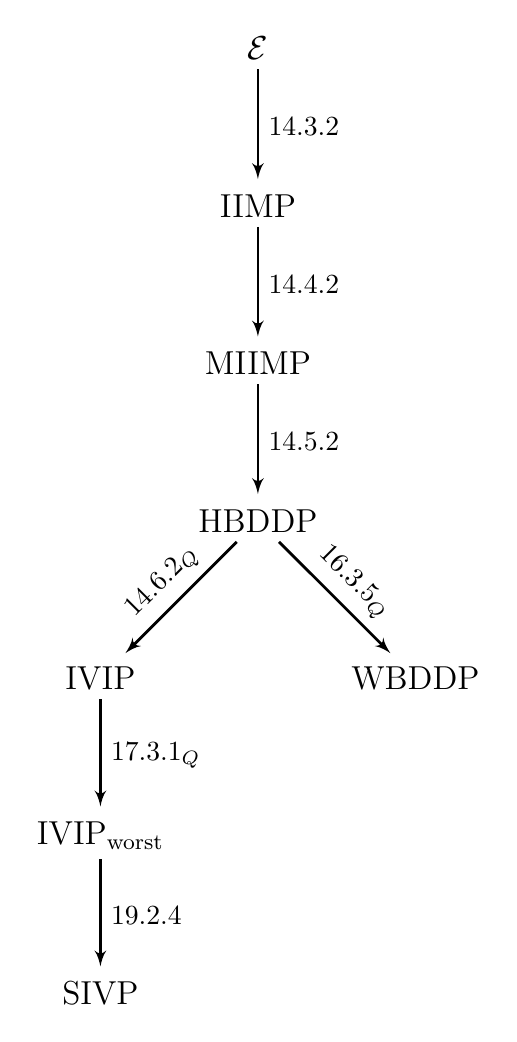
\begin{tikzpicture} [node distance = 2cm, auto, shorten >=2pt]

        \node[font=\fontsize{12}{144}\selectfont] (E) {$\mathcal{E}$};
        \node[font=\fontsize{12}{144}\selectfont] (IIMP) [below of=E] {$\text{IIMP}$};
        \node[font=\fontsize{12}{144}\selectfont] (MIIMP) [below of=IIMP] {MIIMP};
        \node[font=\fontsize{12}{144}\selectfont] (HBDDP) [below of=MIIMP] {HBDDP};
        \node[font=\fontsize{12}{144}\selectfont] (d) [below of=HBDDP] {};
        \node[font=\fontsize{12}{144}\selectfont] (WBDDP) [right of=d] {WBDDP};
        \node[font=\fontsize{12}{144}\selectfont] (IVIPa) [left of = d] {IVIP};
        \node[font=\fontsize{12}{144}\selectfont] (IVIPw) [below of=IVIPa] {IVIP$_{\text{worst}}$};
        \node[font=\fontsize{12}{144}\selectfont] (SIVP) [below of=IVIPw] {SIVP};


        \path [line, line width = 1pt] (E) edge node[right]{14.3.2} (IIMP) ;
        \path [line, line width = 1pt] (IIMP) edge node[right]{14.4.2} (MIIMP);
        \path [line, line width = 1pt] (MIIMP) edge node[right]{14.5.2} (HBDDP);
        \path [line, line width = 1pt] (HBDDP) edge node[sloped, anchor = center, above] {16.3.5$_Q$} (WBDDP);
        \path [line, line width = 1pt] (HBDDP) edge node[sloped, anchor = center, above] {14.6.2$_Q$} (IVIPa);
        \path [line, line width = 1pt] (IVIPa) edge node[right]{17.3.1$_Q$} (IVIPw);
        \path [line, line width = 1pt] (IVIPw) edge node[right] {19.2.4} (SIVP);


        \end{tikzpicture}

        \caption{The chain of reductions given in Gentry's thesis which base security of $\mathcal{E}$ off of worst-case SIVP (or alternatively, WBDDP). An arrow $A \to B$ reads as ``$B$ is reducible to $A$.'' Each arrow is labeled with a reference to the corresponding reduction in Gentry's thesis; a subscript of $_Q$ indicates that the reduction requires a quantum algorithm.}
\end{figure}

        In this section, we will present these above computational problems, but will not give the reductions in detail. A full presentation of the reductions is outside of the scope of this thesis; this section is meant to serve as a guide to following Gentry's reductions.

        The first computational problem is the \emph{Inner Ideal Membership Problem}, or IIMP.

        \begin{definition} [$\gamma$-IIMP]
            Set a ring $R$, ideal $I \subset R$ with basis $\B_I$, and algorithm ${\sf IdealGen}$ as in the encryption scheme. Sample $\B_J^{pk}$ from ${\sf IdealGen}$. Choose a bit $b$ uniformly. If $b = 0$, then set $x \leftarrow D_{\B_I, \gamma, \mathbf{0}}$. If $b = 1$, set $x \leftarrow D_{R, \gamma, \mathbf{0}}$. Then, set $t = x \bmod \B_J^{pk}$. The challenge is to guess $b$ given $\B_J^{pk}$ and $t$.
        \end{definition}

        (In the above definition, sampling from $D_{R, s_{\sf IIMP}, \mathbf{0}}$ means sampling from $\Z^n$ directly, through the standard basis.)

        The security of $\mathcal{E}$ with Gaussian parameter $s = \sqrt{2} \cdot \gamma$ follows directly from the hardness of $\gamma$-IIMP. That is, if there exists an adversary $A$ that breaks the security of $\mathcal{E}$ with non-negligble probability, then there exists an adversary $B$ for the above problem with non-negligible advantage. For this reduction to work, we also require that $s / 2$ is larger than the smoothing parameter of $I$.

        The reduction closely resembles the reduction from the Ideal Coset Problem given in Section \ref{sec:security}. The role of ${\sf Samp}_R \bmod \B_J^{pk}$ as in the ICP is being played here by $D_{\B_I, \gamma, \mathbf{0}} \bmod \B_J^{pk}$, and the role of ${\sf Uniform}(R \bmod \B_J^{pk})$ as in the ICP is being played by $D_{R, \gamma, \mathbf{0}} \bmod \B_J^{pk}$.

        When an adversary $A$ for $\mathcal{E}$ asks for an encryption of either $\pi_0$ or $\pi_1$, the adversary $B$ for IIMP picks a bit $\beta \leftarrow \{0,1\}$, samples a value $v \leftarrow D_{\B_I, \gamma, - \pi_\beta}$, and sends to $A$ $\phi = (\pi_\beta + t + v) \bmod \B_J^{pk}$ (with $t$ as in the above problem), to which $A$ responds with a guess bit $\beta'$. Then, $B$ guesses $b' = \beta \oplus \beta'.$ When $b = 0$, $\phi$ is negligibly close to a valid encryption of $\pi_0$; thus, $A$ will guess $\beta' = 0$, so $B$ will correctly guess $b' = 0$. When $b = 1$, $\phi$ will appear uniformly random to $A$, so $A$ will have advantage zero; thus, $B$ has advantage half of the advantage of $A$.

        \vspace{2em}

        The next step of the chain of reductions is the \emph{modified IIMP} (MIIMP), which is essentially the same as the IIMP, except that $x$ is allowed to be arbitrarily picked from $I$ and $R$ respectively, as long as $|x| \leq \gamma$. The challenge for MIIMP is given $\B_J^{pk}$ and $t = x \bmod \B_J^{pk}$, distinguish the two scenarios. (This corresponds to the condition that $x$ is sampled with Gaussian parameter $\gamma$ in the IIMP.) The reduction boils down to adding a suitable Gaussian to the challenge vector $t$ of MIIMP, in order to create $t'$; the statistical noise from the Gaussian will drown out any difference between the IIMP and MIIMP, but will not change whether $x$ came from $I$ or $R$.

        \vspace{2em}

        The next computational problem is the \emph{Hybrid Bounded Distance Decoding Problem} (HBDDP), defined below:
        \begin{definition} [$\gamma$-HBDDP]
            Fix a ring $R$, ideal $I$, basis $\B_I$ of $I$, and ${\sf IdealGen}$ as in $\mathcal{E}$. Sample $\B_J^{pk}$ from ${\sf IdealGen}.$ Then, the challenger sets $x$ such that $|x| < \gamma$ and sets $t = x \bmod \B_J^{pk}$. The challenge is to output $x$ given $\B_J^{pk}$ and $t$.
        \end{definition}

        The reduction from HBDDP to MIIMP allows us to consider \emph{search problems} instead of descision problems, such as MIIMP.

        As a sidenote, Gentry defines a worst-case version of the above problem, which makes no mention of $\mathcal{E}$:
        \begin{definition} [$\gamma$-WBDDP]
            Fix $R$ and ideal lattice $M \subset R$ with basis $\B_M$. The challenger picks $t$ such that the distance from $t$ to $M$ is at most $\gamma$. The challenge is to, given $\B_M$, find $y \in t + M$ such that $|y| \leq \gamma$.
        \end{definition}

        If we write $t = m + e$, where $m \in M$ and $e < \gamma$, then the challenge is to recover $m$ from $t$, since $(t - m) = e$ is our candidate $y$. This shows why the problem is named ``bounded distance decoding'': we are given a $t$ some bounded distance way from $M$, and are asked to decode the lattice point closest to $t$.

        Gentry proves that if an adversary can solve HBDDP over a non-negligible fraction of bases output by ${\sf IdealGen}$, then an adversary can solve WBDDP over \emph{all} bases $M$ (with determinant bounded by a parameter in ${\sf IdealGen}$). This result depends on an instantiation of ${\sf IdealGen}$ that carries the properties outlined at the end of Section \ref{subsec: mods}.

        It turns out that one must use a factoring oracle in the instantiation of ${\sf IdealGen}$, which means that this is a quantum reduction. The reason a factoring oracle is needed is that to reduce WBDDP to HBDDP, one must take as input an instance $(\B_M, t)$ of WBDDP and output an instance $(\B_J^{sk}, t)$ of HBDDP, such that if the answer $x$ to HBDDP has norm less than $\gamma$, then the answer $y$ to WBDDP has norm less than $\gamma$ -- subject to the worst-case to average-case reduction. This problem turns out to require producing ``small'' principal ideals that one can feed into the HBDDP problem. The way Gentry solves this problem is to pick a random vector $w$ from $\Z^n$, factor $w$, and choose its smallest factor to be the generator of the ideal.

        The main theorem of Gentry's thesis is not basing security on WBDDP, but instead basing security on SIVP. However, some discussion on the hardness of WBDDP itself can be found in Gentry and Halevi's 2011 implementation of the present scheme \cite{gh11implementing}.

        Gentry gives a similar quantum reduction from the \emph{Independent Vector Improvement Problem:}
        \begin{definition} [$\gamma$-IVIP]
            Fix a ring $R = \Z[x] / f(x)$ and ideal lattice $J$ with basis $\B_J$. The challenge is to, given $\B_J$, output an independent set $\B_{J ^{-1}}$ of vectors in the fractional ideal $J \inv$ such that $|\B_{J \inv}| \leq 1/\gamma.$
        \end{definition}

        Recall that given an ideal $J$, the corresponding \emph{fractional ideal} $J \inv$ is the set of all elements in $\mathbb{Q}[x] / f(x)$ such that $J \cdot J\inv = R$. Since $J \inv$ contains fractional elements, the standard basis $\{\mathbf{e}_i\}$ is a trivial solution to the above problem when $\gamma = 1$. Setting $\gamma$ to be larger rules out this triviality.

        First, Gentry proves in $14.6.2$ that IVIP admits a quantum reduction to HBDDP, in the average case. This quantum algorithm invokes Regev's result that a quantum algorithm can use bounded-distance decoding to sample short vectors from the dual lattice. Then, in $17.3.1$, Gentry proves (in a manner identical as for WBDDP) that the IVIP is reducible worst case to average case. Again, this depends on the specific construction of ${\sf IdealGen}$, and involves a quantum factoring algorithm.

        Finally, in Chapter 19, Gentry gives the final reduction, showing that any adversary that can solve IVIP for all ideals (again subject to a size requirement) can solve SIVP, reproduced below:
        \begin{definition} ($\gamma$-SIVP)
            Given a basis $\B$ of a lattice $L$, output a basis $\B'$ of $L$ such that $\Vert \B' \Vert \leq \gamma \cdot \lambda_n(L)$.
        \end{definition}

        One may be worried that the above reductions are made in the quantum setting. After composing quantum reductions, the main security result is not that ``if SIVP is hard for classical computers, then $\mathcal{E}$ is secure'', but rather ``if SIVP is hard for quantum computers, then $\mathcal{E}$ is secure.'' Clearly, the second assumption is stronger. However, as discussed in Section \ref{sec: svpresults}, it is safe to assume that SIVP (along with other classic lattice problems) cannot be solved efficiently with a quantum algorithm for $\gamma$ polynomial in the dimension. However, it is still better to obtain classical reductions rather than quantum reductions, if only to assume as little as possible. (For example, in Chapter \ref{chap: lwe}, we will discuss the \emph{learning with errors} problem, from which is it possible to reduce classically from GapSVP.)

\section{Improving Gentry's Scheme} \label{sec:improvinggentry}
    In this section, we will outline a selection of papers which gave improvements directly relating to Gentry's scheme. A few of these works are tweaks to the Gentry scheme itself, while others have a direct link to Gentry's scheme, but could be considered a separate scheme.

    \subsection{The SV and GH Schemes}
    The first of these papers is due to Smart and Vercauteren, who provide a scheme which can be thought of a reformulation of Gentry's scheme \cite{SV09}. Recall that in Gentry's scheme, we generate a principal ideal $J = \langle s \rangle$, and set the secret key $\B_J^{sk}$ to be the corresponding rotation basis. Then, we generate the public key $\B_J^{pk}$ to be the Hermite normal form ${\sf HNF}(\B_J^{sk})$. (This is before squashing the decryption circuit.) Then, the central computational assymetry is that $\B_J^{pk}$ is a much poorer basis of the lattice than $\B_J^{sk}$, which in turn means that no polytime adversary can use the public key to gain information on ciphertexts. Among other limitations to Gentry's scheme is the size of the public key and ciphertexts. The public key is given directly as a basis, which has size $n^2$, and each ciphertext is a vector of size $n$. For security to hold, $n$ must be very large; thus, we obtain even larger public keys.

    A large insight of Smart and Vercauteren is that one may instead give an \emph{algebraic} representation of the public key; in the Gentry scheme, the fact that $J$ is a principal ideal is not used in the construction of the public key.

    Let $F(x)$ be a monic irreducible polynomial of degree $N$, possessing a root $\theta$. (In practice, they set $F(x) = x^{2^n} + 1$.) Then, we can consider the ring $\Z[\theta] = \Z[x] / (x - \theta)$, which consists of polynomials $C(\theta) = \sum_{i = 0}^{N-1} c_i \theta^i$. We will generate a random polynomial $G(x)$, and consider the ideal $\mathfrak{p} = \langle G(\theta) \rangle$. (This ideal $\mathfrak{p}$ is analogous to $J$.) Then, the trick is that we will \emph{also} be able to write that
    \[\mathfrak{p} = \langle p, \theta - \alpha \rangle, \]
    where $p$ is an integer and $\alpha$ is an element of $\Z_p$. That is, computing modulo $\mathfrak{p}$ means computing modulo $p$ and evaluating every polynomial $C(x)$ at $\alpha$.


    The public key consists of the information $(p, \alpha)$, and the secret key contains information about $G(\theta) \inv$. For a message $M \in \{0, 1\}$, encryption consists of creating the polynomial $C(x) = M + 2 R(x)$, and outputting $c = C(\alpha) \bmod p$. (I.e, the ciphertext $c$ is equal to $M + 2R(x)$ modulo the ideal $\mathfrak{p}$.) Then, given the single generator $G(\theta)$ of $\mathfrak{p}$, one can derive $C(x)$ from $c$, since we know that $c - C(\theta) \in \mathfrak{p}$, so $c - C(\theta) = q(\theta) \cdot G(\theta)$; from here, decryption follows, since we can divide by $G(\theta)$ to compute $q(\theta)$. The main advantage of their scheme is that the public key consists only of $p$ and $\alpha$, and ciphertexts are polynomials reduced modulo $\mathfrak{p}$, which in practice are smaller than the ciphertexts of Gentry's scheme.

    The central computational assymetry here is that without information about $G(\theta)$, one cannot carry out the above process. Their hardness assumption, then, is the \emph{Small Principal Ideal Problem}, which is essentially to compute $G(\theta)$ given $p$ and $\alpha$.

    Notably, this construction scales to larger message spaces; we could generate messages $M(x)$, which are polynomials of degree $N$ with binary coefficients. Then, we similarly compute $C(x) = M(x) = 2 R(x)$, and decrypt using $G(\theta) \inv$. Because of this, we can consider \emph{SIMD} (Single Instruction, Multiple Data) operations, where single arithmetic operations would compute on \emph{vectors} of messages, all at once. Smart and Vercauteren make this idea more precise for their scheme in \cite{SV09-2}, where they give an example of computing AES homomorphically using vectorized messages.

    In \cite{SV09}, Smart and Vercauteren describe how to turn their somewhat homomorphic scheme into a fully homomorphic one, essentially following the same outline as Gentry. However, in practice they were unable to carry out homomorphic decryption. The issue was key generation: to obtain a somewhat homomorphic scheme with large enough circuit depth to support homomorphic decrypt, they needed $N$ to be on the order of $2^{27}$; however, they were unable to generate keys for $N$ greater than $2^{12}$. Their key generation algorithm generated the ideal $\mathfrak{p}$ probabilistically, by choosing $G(x)$ at random and checking whether $G$ satisfied the necessary conditions; as $N$ increases, it becomes less likely to pick a correct $G(x)$ at random.

    This scheme is improved upon by Gentry and Halevi in 2011 \cite{gh11implementing}. Among other things, they improve upon two inefficiencies in the above scheme: first, they employ a FFT-based polynomial inversion algorithm to obtain $G(\theta) \inv$ from $G(\theta)$; secondly, they point out that one can use a faster, recursive formula to evaluate $C(\theta)$ from $C(x)$ during encryption. Due to their optimizatons, they were able to execute a bootstrapping operation. Depending on their security settings, their public keys ranged from 70 megabytes to 2.3 gigabytes, with a bootstrapping operation taking from 30 seconds to 30 minutes.

    \subsection{Other Results}

    In 2010, Stehl\'e and Steinfeld present a refined analysis of Gentry's bootstrapping procedure, discussed in Section \ref{sec:squash} and in Section \ref{sec:dghvsquash} of the next chapter \cite{Stehle2010}. Recall in the squashed scheme, the public key includes a set $\{t_i\}_{i = 1}^{\gamma_{set}(n)}$ random-looking vectors, with a subset $S$ of cardinality $\gamma_{subset}(n)$ that sums to the secret $\mathbf{v}_{sk}$, which is used for decryption. These $\{t_i\}$ live in $J \inv \bmod \B_I$, so are fractional vectors, and must be represented with some amount of bits of precision. As we show in Section \ref{sec:dghvsquash} of the next chapter, Gentry fully computes the sum $\sum_{i \in S} t_i$ homomorphically. However, since this sum is only needed to be correct modulo $2$, Stehl\'e and Steinfeld show that many significant bits of the $t_i$ do not need to be summed together, since they will not contribute to the sum modulo $2$. In total, their methods lead them to a $\widetilde{O}(\lambda^{3.5})$ computation complexity per homomorphic addition or multiplication. This analysis applies to any FHE scheme which follows Gentry's construction for bootstrapping.



\chapter{Fully Homomorphic Encryption over the Integers} \label{chap:dghvchap}
In this chapter, we outline developments following Gentry's initial scheme, but before the LWE based schemes in the next chapter. In these schemes, the same general outline is followed: a somewhat homomorphic encryption scheme in constructed, and then bootstrapping is applied by squashing the decryption circuit. However, in general these schemes are much more compact, and refer to hardness assumptions that do not interface directly with lattices.


\section{Statistical Preliminaries}
\label{sec:statprelim}
The definitions below are given to present a simplified form of the \emph{leftover hash lemma}, quoted from \cite{ILL}. This result will be used throughout the rest of the thesis. For our purposes, the intended use is as follows: given a collection of uniformly random vectors $\vec{a}_i \leftarrow \Z_q^n$, a uniformly random subset sum of them, $\sum_i s_i \vec{a}_i$, where each $s_i \leftarrow \{0,1\}$, again looks like a uniformly random vector. (In full generality, the leftover hash lemma says something stronger \cite{haastad1999pseudorandom}, but we will not consider that here.)

The \emph{statistical distance} $\delta(X, Y)$ between two distributions $X$ and $Y$ (with numeric outputs) over a finite domain is defined to be $\frac{1}{2} \sum_x \left| \Pr[X = x] - \Pr[Y = x] \right|$. If $\delta(X, Y)$ is negligible, no computational adversary with oracles to $X$ and $Y$ can distinguish the two distributions with non-negligible probability.

Then, the relevant lemma is the following:
\begin{lemma}{Matrix Leftover Hash Lemma.}
    Let $\kappa \in \N$, $n \in \N$, $q \in \N$, and $m \geq n \log q + 2 \kappa$. Let $\vec{A} \leftarrow \Z_q^{m \times n}$ be a uniformly random matrix, let $\vec{r} \leftarrow \{0,1\}^m$ and let $\vec{y} \leftarrow \Z_q^n$. Then,

    \[\delta((\vec{A}, \vec{A}^T\vec{r}), (\vec{A}, \vec{y})) \leq 2^{-\kappa}.\]
\end{lemma}

The present scheme will only need to invoke the above lemma in the case when $n = 1$; in this setting, the above lemma states that given a collection of uniformly random numbers $\{x_i\}_{i = 1}^m \leftarrow \Z_q$, a random subset sum $\sum_i s_i x_i$ of these numbers again appears uniformly random. (Intuitively, this is because there are $2^m$ possible different subset sums, so no computational adversary can recognize all of them when $m$ is large enough.)

(We will invoke the lemma for $n>1$ in the next chapter.)


\section{Intuition}
\label{sec:integers}
Very soon after Gentry's initial construction a new, much more simple scheme was presented by van Dijk, Gentry, Halevi, and Vaikuntanathan (DGHV). The scheme may be found in \cite{dghv}. First, we outline the general idea of the DGHV scheme. We then present the scheme in full detail in \ref{sec: dghvscheme}. In Section \ref{sec: dghvsecurity}, we present the relevant hardness assumption, give the corresponding reduction, and discuss lattice-based attacks. In Section \ref{sec: dghvcomplexity}, we evaluate the scheme, in terms of both computational complexity and space considerations.


Recall that Gentry's somewhat homomorphic scheme had this general outline: given a plaintext $\pi$, introduce some ``error'' encoded as a point in $\pi + I$, where $I$ is an ideal from some ring. One can also think of $\pi' \in \pi + I$ as an encoding of $\pi$ as the distance to the lattice corresponding to $I$, since $\pi' \bmod I = \pi$. Then, reduce $\pi'$ by some public, hard-to-compute-with basis $\B_J^{pk}$ to obtain $c$. Thus, $c \bmod J = \pi'$, from which we can compute $\pi$ to be $(c \bmod J) \bmod I$. However, the public basis $\B_J^{pk}$ is inadequate to compute $c \bmod J$; this can only be done with the secret basis $\B_J^{sk}$.

The DGHV scheme can be thought of as a simplified version of the above idea. Throughout, we will be working over $\Z$, with $I = 2\Z$. Thus, the plaintext space is equal to $\Z / 2\Z;$ i.e., our messages are single bits. Then, we set $J = p\Z$, where $p$ is some sufficiently large random odd integer. This $p$ is our secret key. To send $\pi$ along $I$, we simply compute $\pi + 2r$, where $r$ is some sufficiently large random integer. Thus, an element of $\pi + I + J$ is represented by $\pi + 2r + kq$.

Our goal is to give an adversary the ability to construct a ciphertext of the form $\pi + 2r + kq$, but \emph{not} permit that adversary to compute $c \bmod p$. One tempting solution to this problem is to consider $pq \Z$ a ``bad basis'' of $p \Z$, with large $q$: computing $c \bmod pq$ is analogous to computing $c \bmod \B_J^{sk}$ as in the Gentry scheme, since both give ``poor reductions'' of $c$. However, semantic security does not follow analogously, since any selection of $c \in \pi + pq \Z$ can be undone with $c \bmod pq$.

This means that we will need an alternate way to think about $J$. The problem with the above proposal is that the adversary knows that $pq$ will always be the least common multiple of $kp$ present in each ciphertext. This means that we actually want a way for the adversary to generate $c = \pi + 2r + kp$, but simultaneously, have the distribution of possible $k$s not leak any information to the adversary. If the adversary cannot predict $k$, the adversary should not be able to decrypt $c$.

To achieve this, we will give a \emph{noisy} description of $J$. First, we include in the public key a set $\{z_i\}$ of many encryptions of zero: that is, each $z_i$ is equal to $2r_{i} + k_{i}p$, for uniformly random $k_i$ and $r_i$. Then, to generate a ciphertext of the correct form, we compute $\pi + 2r$ for uniformly random $r$, and add a \emph{subset sum} of the $\{z_i\}$:
\[\pi \to \pi + 2r + \sum_{i \in S} z_i \bmod P,\]

where $S$ is a subset of indices into $\{z_i\}$ chosen uniformly at random, and $P$ is a public, large parameter computed from $p$. Correctness of decryption follows as long as the randomness present in $r$ and in each $r_i$ does not sum to greater than $p$.

Intuitively, this scheme is secure because each possible resultant $k$, computed from all of the $k_i$ for $i$ in $S$, looks uniformly random for each possible $S$. Since there are exponentially many possible index sets $S$, this $k$ cannot be efficiently predicted by a computational adversary. This result will invoke the leftover hash lemma, presented in Section \ref{sec:statprelim}.


The above is only a sketch: in the actual construction, we do not compute the $\{z_i\}$, but instead compute samples $\{x_i\}_{i = 1}^{\tau}$ from the following distribution, which depends on parameters $\gamma$ and $\rho$:

\[\mathcal{D}_{\gamma, \rho}(p) = pq+r, \text{where } q \leftarrow \Z \cap [0, 2^\gamma / p), r \leftarrow (-2^\rho, 2^\rho).\]

Since $2 x_i = 2pq + 2r$, we can think of $2 x_i$ as a valid encryption of zero, as above. Then, we set $P$ from above to be the largest of the $x_i$ (subject to a parity condition on $P$).


The corresponding circuits of the homomorphic scheme will be arithmetic circuits over $\Z / 2\Z$. Addition computes XOR, and multiplication computes AND. By generating encryptions of $1$, we can compute NOT, since $m \oplus 1 = \neg m$.



\section{Construction of the Scheme}
\label{sec: dghvscheme}

As demonstrated above, we will need several constants to quantify the randomness in the scheme.
\begin{itemize}
\item $\eta$ upper bounds the bit length of $p$, the secret key.
\item $\gamma$ and $\rho$ parametrize the randomness in $\mathcal{D}_{\gamma, \rho}(p)$, bounding the length of $q$ and $r$ respectively.
\item $\tau$ parametrizes the number of integers in $\mathbf{x}$, the public key.
\end{itemize}

The above parameters have required asymptotics in the security parameter, $\lambda$; some requirements are to maintain security, while other requirements are to enable the somewhat homomorphic scheme to be bootstrapped. We will discuss each requirement in its relevant section.

\begin{itemize}
\item $\rho = \omega(\log \lambda)$.
\item $\rho' = \rho + \omega(\log \lambda)$. (This serves the same basic purpose as $\rho$, but $\rho'$ is necessary for the security reduction.)
\item $\eta \geq \rho' \cdot \Theta(\lambda \log^2 \lambda)$.
\item $\gamma = \omega(\eta^2 \log \lambda)$.
\item $\tau \geq \gamma + \omega(\log \lambda)$.
\end{itemize}

One can think of setting parameters as follows:
\begin{itemize}
    \item $\rho = \lambda$,
    \item $\rho' = 2\lambda$,
    \item $\eta = \widetilde{O}(\lambda^2)$,
    \item $\gamma = \widetilde{O}(\lambda^5)$, and
    \item $\tau = \gamma + \lambda$.
\end{itemize}

Now, we discuss the somewhat homomorphic encryption scheme.
\begin{description}
\item[Keygen] randomly selects an odd integer $p$ from the range $[2^{\eta - 1}, 2^\eta)$. The secret key is $p$. To compute the public key, sample $x_i \leftarrow \mathcal{D}_{\gamma, \rho}(p)$, for $i = 0, \dots, \tau$. Relabel so that $x_0$ is the largest. Until $x_0$ is odd and $x_0 \bmod p$ is even, recompute the $x_i$. The public key is $\mathbf{x} = \{x_0, \dots, x_\tau\}$.
\item[Encrypt] takes as input $m \in \{0, 1\}$ and $pk = \mathbf{x}$. Choose a random subset of indices $S \subseteq \{1, 2, \dots, \tau\}$, and a random integer $r$ in $(-2^{\rho'}, 2^{\rho'})$. Compute $m' = m + 2(r + \sum_{i \in S} x_i)$, and return the ciphertext $c = m' \bmod x_0$.

Note that the noise $r$ introduced here is at most $2^{\rho'}$, so is generally much larger than the noise coming from $\mathcal{D}_{\gamma, \rho}$.

\item[Evaluate] takes as input $pk$, $C$, and input ciphertexts $c_i$, and performs the arithmetic operations corresponding to $C$ on the $c_i$, and returns the result.
\item[Decrypt] takes as input $sk = p$, and $c$. It returns $m = (c \bmod p) \bmod 2$. ($c \bmod p$ is computable as $c - p \lfloor c / p \rceil$.)

\end{description}

We must now show that decryption and evaluation are correct, for permitted circuits $\mathcal{C}_\mathcal{E}$.
\subsection{Correctness and Permitted Circuit Complexity} \label{sec:dghv_correctness}
First, consider ciphertexts output by ${\sf Encrypt}$. We can prove the following lemma:
\begin{lemma}
Let $(pk, sk) \leftarrow$ ${\sf KeyGen}$, and let $c \leftarrow \Enc_{pk}(m)$. Then $c = ap + (2b + m)$ for integers $a$ and $b$, with $|2b+m| \leq \tau 2^{\rho + 3}.$
\end{lemma}

The above lemma shows that with proper setting of parameters, decryption is correct on fresh ciphertexts. If $\tau 2^{\rho + 3}$ is sufficiently smaller than $p$ (we will require $p/8$), we obtain that $c \bmod p = 2b+m$, so $(c \bmod p) \bmod 2 = m$.
\begin{proof}
To show the above, note that $c = m + 2r + 2\sum_i x_i \bmod x_0$. Since $x_0$ is the largest $x_i$ and there are $\tau$ total $x_i$ we get that
\[c = m + 2r + 2\sum_i x_i + kx_0,\]
with $|k| \leq \tau$.

Since each $x_i = pq_i + r_i$, we get that
\[c = p(kq_0 + 2\sum_i q_i) + (m + 2r + kr_0 + 2\sum_i r_i).\]

The left hand side is our $a$. Now, we require in ${\sf KeyGen}$ that $x_0 \bmod p$ is even, so $kr_0$ is even. Thus, $2r + kr_0 + 2\sum_i r_i$ is even, so the right hand side can be written as $2b+m$. Regarding the norm of the right hand side,
\[|m + 2r + kr_0 + 2\sum_i r_i| \leq 1 + 2\cdot 2^{\rho'} + \tau 2^\rho + 2 \cdot \tau 2^\rho \leq 8\tau2^\rho \leq \tau2^{\rho' + 3}. \]
\end{proof}


Now, we define the set of permitted circuits. Given a circuit $C$, the corresponding \emph{arithmetic circuit} $C'$ over $\Z$ has each boolean gate replaced by the corresponding arithmetic gate. For example, if $C = (x_1 \wedge x_2) \oplus x_3$, then the corresponding arithmetic circuit is $(x_1 \cdot x_2) + x_3$.



\begin{definition} (Permitted Circuit) \label{def:permcircuit}
$\mathcal{C}_\mathcal{E}$ is the set of circuits such that for any $\alpha \geq 1$ and any set of integer inputs with norm at most $\tau 2^{\alpha(\rho' + 3)}$, the corresponding arithmetic circuit has output with norm at most $2^{\alpha(\eta - 4)}.$
\end{definition}

(The above definition of permitted circuit is altered from the original paper, in order to aid analysis.)


Using the above definition for $\mathcal{C}_\mathcal{E}$, we can show the following lemma, which implies correct circuit evaluation:
\begin{lemma} \label{lem:ciphertextbound}
Let $(pk, sk) \leftarrow$ ${\sf KeyGen}$. Let $C \in \mathcal{C}_\mathcal{E}$ with $t$ inputs $m_1, \dots, m_t$, with $m_i \in \{0, 1\}$. Let $c_i$ be an encryption of $m_i$, let $m = C(m_1, \dots, m_t)$, and $c \leftarrow {\sf Evaluate}_{pk}(C, c_1, \dots, c_t)$. Then, $c = ap + (2b + m)$ for integers $a, b$ with $|2b + m| \leq p/8$.
\end{lemma}
\begin{proof}
Let $C'$ denote the circuit over $\Z$ corresponding to $C$. By above, each $c_i$ is equal to $a_ip + (2b_i + m_i)$. Then, note that
\[c_i + c_j = (a_i + a_j)p + (2(b_i + b_j) + (m_i + m_j)) \in 2A + (m_i + m_j) + p\Z\]
and
\[c_ic_j \in (2b_i + m_i)(2b_j + m_j) + \Z p = 2B + m_i m_j + p\Z,\]

where $A$ and $B$ are some integers smaller than $p$.

Since $C'$ is comprised of multiplications and additions, this implies that
\[C'(c_1, \dots, c_t) \in C'(2b_1 + m_1, \dots, 2b_t + m_t) + p\Z.\]

Thus, $C'(c_1, \dots, c_t) \bmod p$ has the same parity as $C(m_1, \dots, m_t)$. Thus, $c = ap + (2b + m)$, for some integer $a$ as in the last line.

This $2b + m$ is exactly equal to $C'(2b_1 + m_1, \dots, 2b_t + m_t)$. Since each $2b_i + m_i \leq \tau 2^{\rho' + 3}$, by the above lemma and since $C \in \mathcal{C}_\mathcal{E}$ (with $\alpha = 1$), we have that $C'(2b_1 + m_1, \dots, 2b_t + m_t) \leq 2^{\eta - 4}.$ Since $p \leq 2^\eta$, we can upper bound this quantity by $p / 8$.
\end{proof}


For convenience, we may express homomorphic computations in terms of permitted (multivariate) \emph{polynomials} over $\mathbf{F}_2$, rather than permitted circuits. Here, depth of polynomial corresponds to degree of the corresponding circuit.

\begin{lemma} (Permitted Polynomial) \label{lem: permpoly}
Let $f(x_1, \dots, x_t)$ be a polynomial over $\mathbf{F}_2$, computing an arithmetic circuit $C'$. If $|f| \cdot (\tau 2^{\rho' + 3})^d \leq 2^{\eta - 4}$, (where $|f|$ is the $\ell_1$ norm of the coefficient vector of $f$) then $C'$ has a corresponding permitted circuit $C \in \mathcal{C}_\mathcal{E}$.
\end{lemma} %also changed to adapt my def

This directly suggests a definition of permitted polynomial:
\begin{definition} (Permitted Polynomial) \label{def: permpoly}
A polynomial $f(x_1, \dots, x_t)$ over $\mathbf{F}_2$ is a permitted polynomial if its degree $d$ is bounded by:
\[d \leq \frac{\eta - 4 - \log |f|}{\rho + 3 + \log \tau}.\]
\end{definition}


\section{Reduction from Approximate GCD}
\label{sec: dghvsecurity}

Next, we show security for the above somewhat homomorphic scheme.

To decrypt, one needs to obtain $p$; however, the adversary only has the $\{x_i\}$ from the public key. The \emph{approximate GCD} (AGCD) problem is exactly this problem:
\begin{definition} (Approximate GCD)
The $(\rho, \eta, \gamma)$-approximate GCD problem is: given polynomially many samples from $\mathcal{D}_{\gamma, \rho}(p)$ for an $\eta$-bit random odd integer $p$, output $p$.
\end{definition}

Discussion of the hardness of Approximate GCD is deferred to the end of this section.

We reduce the above problem to the security of our scheme:

\begin{theorem}
Any PPT adversary $A$ attacking the DGHV scheme with advantage $\varepsilon$ and parameters $(\rho, \eta, \gamma, \tau)$ can be turned into a PPT adversary $B$ attacking the $(\rho, \eta, \gamma)$-approximate GCD problem with advantage at least $\varepsilon / 2$.
\end{theorem}
\begin{proof}
For this section, for integers $z, p$ write $q_p(z)$ to be the quotient of $z$ by $p$, and $r_p(z)$ to be the remainder.


The idea of the proof is that given a correct public key (which $B$ will be able to supply with non-negligible probability), $A$ can be used to construct an oracle for $q_p(z) $ for any $z$. This can be used to compute $p$. The below proof will be given in three steps:
\begin{enumerate}
\item Computing a correct public key from $(\rho, \eta, \gamma)$ given to $B$.
\item Constructing an oracle for $q_p(\cdot) \bmod 2$ from $A$.
\item Computing $p$ from the above oracle and a correct public key.

\end{enumerate}


\subsection{Computing a Public Key}
$B$ obtains $\tau + 1$ samples $x_0, \dots, x_\tau$ from $\mathcal{D}_{\gamma, \rho}$, and relabels so that $x_0$ is the largest. If $x_0$ is even, $B$ restarts. Then, $B$ gives the public key $\mathbf{x} = x_0, \dots, x_\tau$ to $A$.

With probability close to $\frac{1}{2}$, $r_p(x_0)$ will be even, and the above will be a correct public key, which $B$ gives to $A$.


\subsection{Constructing the Oracle from $A$}
We now show how, given a correct public key, $A$ can be used to create an oracle for $q_p(z) \bmod 2$, as long as $z \in [0, 2^\gamma)$ and $|r_p(z)| < 2^\rho$. (Note here that the noise of $z$ is required to be less than $2^\rho$, not less than $2^{\rho'}$.)

\begin{enumerate}

\item Do the following $\text{poly}(\lambda) / \varepsilon$ times, where $\varepsilon$ is the advantage of $A$:
	\begin{enumerate}
	\item Uniformly choose: $r$ $\leftarrow$ $(-2^{\rho'}, 2^{\rho'})$, $S \subseteq \{1, \dots, \tau\}$. %why do we need m?
	\item Compute $m' = z + 2(r + \sum_{i \in S} x_i)$, and $c = m' \bmod x_0$.
	\item Give $c$ to $A$, to obtain guess bit $a$.
	\item Let $b = a \oplus {\sf parity}(z)$.
	\end{enumerate}
\item Output the majority over all $b$'s computed in the above iterations.
\end{enumerate}

(Notice that when $A$ has non-negligible advantage, $\text{poly}(\lambda) / \varepsilon$ is a polynomial.)

We now have that $c$ is with all but negligible probability a valid encryption of the bit $r_p(z) \bmod 2$:
\begin{lemma} \label{lem: validenc}
	Fix public and secret keys $sk = p, pk = \{x_0, \dots, x_\tau\}$ as in the KeyGen for DGHV, and let $z = pq_z + r_z$ be a positive integer at most $2^\gamma$ such that $|r_z| \leq 2^\rho$. Then, the two below distributions are negligibly close (with all but negligible probability over the choice of public key):
	 \[\mathcal{C}_{pk}(z) = \left\{ c' \leftarrow \left[z + 2(r + \sum_{i \in S} x_i) \right] \bmod x_0, \text{ where } S \subseteq_R \{1, \dots, \tau \}, r \leftarrow (-2^{\rho'}, 2^{\rho'}) \right\} \]
	 and
	 \[\sf{Encrypt}_{pk}(r_z \bmod 2). \]
\end{lemma}

The proof is omitted here, but can be found in the original paper \cite{dghv}. The idea of the proof is as follows: let $c \leftarrow \sf{Encrypt}_{pk}(r_z \bmod 2)$, and then before reducing modulo $x_0$, break $c$ and $c'$ apart as below:

\[ c' = Q'p + 2R' + m', c = Qp + 2R + m.\]

Then, $pq_z$ will be absorbed into $Q'p$, and $r_z$ will be absorbed into $2R' + m'$; thus, $m' = r_z \bmod 2$. To argue that $c$ and $c'$ are indistinguishable, we argue that they are indistinguishable componentwise (by noise and by coefficient); since $r \ll p$, these components can be taken to be independent.

Regarding the noise, $c$ and $c'$ differ by the inclusion of $r_z$ into $R'$. However, since $|r_z| < 2^\rho$, this statistical difference is drowned out by the inclusion of $r$ both in the first distribution and the encryption scheme, which may be at most $2^{\rho'}$ in magnitude (i.e., superpolynomially larger than $r_z$). That is, no computational adversary can distinguish between randomness stemming from $r_z + 2(r + \sum_{i \in S} r_{x_i})$ (coming from the first distribution) and the randomness coming from $2(r + \sum_{i \in S} r_{x_i})$ (coming from the second distribution).

Regarding the coefficient, the argument is a standard application of the leftover hash lemma. The coefficient $Q'$ coming from the first distribution is equal to $q_z + \sum_{i \in S} q_{x_i}$, while the coefficient $Q$ coming from the second distribution is equal to $\sum_{i \in S} q_{x_i}$. When $\tau$ (the number of $x_i$) is large enough, after reducing modulo $x_0$, $q_z$ becomes indistinguishable from some sum of $q_{x_i}$, since these coefficients wrap around; i.e., $\tau$ is large enough that $Q'$ is plausibly another subset-sum, even though $q_z$ does not have to be equal to one of the $q_{x_i}$.


Thus, with advantage $\varepsilon$, $A$ will output $a = r_p(z) \bmod 2$, which means $b = (r_p(z) \bmod 2) \oplus {\sf parity}(z)$. Since $p$ is odd,
\[{\sf parity}(z) = (r_p(z) \bmod 2) \oplus (q_p(z) \bmod 2),\]
so $b = q_p(z) \bmod 2$. By taking a majority over $\text{poly}(\lambda) / \varepsilon$ votes, we receive a correct oracle with non-negligible probability.



\subsection{Computing $p$}

Suppose we have two integers $z_1 = q_p(z_1) \cdot p + r_p(z_1)$ and  $z_2 = q_p(z_2) \cdot p + r_p(z_2)$, sampled from $\mathcal{D}{\gamma, \rho}(p)$, so that $r_p(z_i) \ll p$. Then, given an oracle $f(z)$ that computes $q_p(z) \bmod 2$. We use $f(z)$ to construct a \emph{modified GCD} algorithm, which we will be able to use to compute $p$.

\subsubsection{Modified GCD}

On input $z_1, z_2$:
\begin{enumerate}
\item Swap so that $z_1 \geq z_2$. If $z_2 = 0$, output $z_1$.
\item Let $b_1 = f(z_1)$, and $b_2 = f(z_2)$.
\item If both $b_1$ and $b_2$ are $1$, set $z_1
\leftarrow z_1 - z_2$ and $b_1 \leftarrow 0$.
\item For $i = 1, 2$, if $b_i = 0$, then set $z_i \leftarrow (z_i - {\sf parity}(z_i)) / 2$.
\item Repeat the above.
\end{enumerate}

This algorithm is similar to the usual binary GCD computation, but the decision to divide by two is given not by the parity of $z$, but the parity of $q_p(z)$. Note that we do \emph{not} multiply the resultant GCD by $2$ if both $b_i$ are $0$.

When we have that $r_p(z_i) \ll p$, we get that the above computes separately on $q_p(z_i)$ and $r_p(z_i)$. In Step 3, if both $b_i$ are $1$, we get immediately that
\[\text{Step 3: } q_p(z_1) \rightarrow q_p(z_1) - q_p(z_2), r_p(z_1) \rightarrow r_p(z_1) - r_p(z_2).\]

In Step 4, subtracting $1$ from $z_i$ will not change $q_p(z_i)$ (since $r_p(z_i) \ll p$) so we get that
\[\text{Step 4: } q_p(z_i) \rightarrow q_p(z_i) / 2, r_p(z_i) \rightarrow (r_p(z_i) - {\sf parity}(z_i)) / 2.\]

The above two steps maintain that $r_p(z_i)$ is much smaller than $p$. In Step 3, $|r_p(z_1)|$ is bound by $\max(r_p(z_1), r_p(z_2))$, and in Step 4, the norm of $r_p(z_i)$ does not increase. Since the norm of $r_p(z_i)$ never increases, the above two steps always compute separately on the quotient and remainder.

Thus, we get that the above operations correspond to the usual GCD computation on the $q_p(z_i)$. Since we do not multiply by $2$ if both $b_i$ are $0$, the output of this algorithm after ${\sf poly}(\gamma)$ iterations is an integer $z'$ where $q_p(z')$ is equal to the \emph{odd part} of ${\sf GCD}(q_p(z_1), q_p(z_2))$. (Given some integer $N = 2^A B$, where $B$ is odd, the odd part of $N$ is equal to $B$.)

\subsubsection{Computing $p$ from Modified GCD}

Sample two integers $z_1$ and $z_2$ through $\mathcal{D}{\gamma, \rho}(p)$, and run the above algorithm on them to obtain an integer $z'$, such that $q_p(z')$ is equal to the odd part of ${\sf GCD}(q_p(z_1), q_p(z_2))$.

With probability close to $6 / \pi^2$ ($1 / \zeta(2)$, the Riemann zeta function) we will have that $q_p(z_1)$ and $q_p(z_2)$ are relatively prime, which means that $q_p(z') = 1$. Thus, we obtain that $z' = p + r$, with $|r| \leq 2^\rho$.

Finally, run the modified GCD algorithm on $z_1$ and $z'$. With high probability, $q_p(z_1)$ will be much larger than $1$ throughout the algorithm, so $z_1$ and $z'$ will never swap in Step 1. Thus, $b_1$ is the parity of $q_p(z_1)$, and $b_2 = 1$. If $b_1 = 1$, we set $z_1 \leftarrow z_1 - z_2$, so $q_p(z_1) \leftarrow q_p \leftarrow 1$. Then, Step 4 always divides $q_p(z_1)$ by $2$, since $b_1$ is set to $0$ in Step 3. Thus, the parity bits of $q_p(z_1)$ obtained from $f(z_1)$ each iteration will spell out $q_p(z_1)$.

Now that we have $q_p(z_1)$, we calculate $p = \lfloor z_1 / q_p(z_1) \rceil$. Since $\rho \leq p^2 \gamma$ (see Section \ref{sec: dghvscheme}), $|r_p(z_1) / q_p(r_1)|$ will be less than $1$ with high probability, so this computation of $p$ is correct.

Thus, given access to an oracle for the parity bit of $q_p(z)$ and the public key, we may reconstruct $p$ with non-negligible probability.

Put together, we have:
\begin{enumerate}
    \item A valid public key, with probability $1/2$
    \item An oracle for $q_p(\cdot) \bmod 2$ that succeeds with non-negligible probability, conditioned on a valid public key
    \item A way to compute $p$, conditioned on the above oracle being correct.
\end{enumerate}

To complete the proof, what remains to be shown is that Step 3 of the above can be composed with Step 2; that is, that we may replace the always-correct oracle in Step 3 with the oracle in Step 2, which succeeds with non-negligible probability each time it is called. This argument is omitted here, but can be found in the original paper \cite{dghv}.

\end{proof}


\section{Bootstrappability} \label{sec: dghvsquashed}
In this section, we show that this scheme may be bootstrapped. The outline is the same as Gentry's scheme: we present a modified scheme that contains a decryption algorithm that is shallow enough to be evaluated by the somewhat homomorphic scheme.

To do this, we first modify the somewhat homomorphic scheme by squashing the decryption circuit. The encryptor precomputes a set $T$ of information that can be used to decrypt, but only if the decryptor knows the secret subset $S$ of this information. This relies on the hardness of sparse subset sum, discussed in the previous chapter. In effect, the role of the decryptor changes from computing $(c \bmod p) \bmod 2$ to computing $\lfloor \sum_i s_i z_i \rceil \bmod 2$, where each $s_i$ is either $0$ or $1$, and each $z_i$ is a fractional number. The former requires a circuit depth too large for the present scheme, while the latter is parallelizable over $i$, which grants a shallower circuit depth.

We introduce three more parameters, and their suggested value:
\begin{enumerate}
\item $\kappa$, which parametrizes the bits of precision in the above fractional numbers; set to $\gamma \eta / \rho'$.
\item $\Theta$, which parametrizes the size of $T$; set to $\omega(\kappa \log \lambda)$.
\item $\theta$, which parametrizes the size of the secret subset $S$; set to $\lambda$.
\end{enumerate}

\begin{description}
\item[KeyGen:] Generate $pk = \mathbf{x}$ and $sk = p$ as in the original scheme. Choose at random a $\Theta$-bit vector $\mathbf{s} = \{s_1, \dots, s_\Theta\}$ with $\theta$ bits nonzero. Let $S = \{i \mid s_i = 1\}$.

Randomly generate integers $u_i \in \Z \cap [0, 2^{\kappa + 1}]$ for $i \in \{0, \dots, \Theta\}$, such that $\sum_{i \in S} u_i = \lfloor 2^\kappa / p \rceil \bmod 2^{\kappa + 1}.$
Then, let $y_i = u_i / 2^\kappa$ and $\mathbf{y} = \{y_i\}$, so that $\sum_{i \in S} y_i \bmod 2 = 1/p - \Delta$, for $|\Delta| < 2^{-\kappa}$.

The secret key $sk'$ is $\mathbf{s}$, and the public key $pk'$ is $(pk, \mathbf{y})$.

\item[Encrypt and Evaluate:] Generate a ciphertext $c$, as in the original scheme. For each $i \in \{0, \dots, \Theta\}$, compute $z_i = c \cdot y_i \bmod 2$; keep only $\lceil \log \theta \rceil + 3$ bits of precision after the decimal point. Output $c$ and $\{z_i\}$.
\item[Decrypt:] Given ciphertext $(c, \{z_i\})$ and secret key $\{s_i\}$, compute $m = (c - \lfloor \sum s_i z_i \rceil) \bmod 2$.
\end{description}


\subsection{Correctness of Squashed Scheme}
Throughout this section, abbreviate $c \bmod 2$ as $[c]_2$.
\begin{lemma}
	The above squashed scheme is correct for permitted circuits of the original scheme, as defined in Definition \ref{def:permcircuit}. Additionally, for every ciphertext $(c, \{z_i\})$ evaluated from a permitted circuit, $\sum s_i z_i$ is within $1/4$ of an integer.
\end{lemma}
\begin{proof}
	To show the scheme is correct for the set of permitted circuits, we need to show that for a ciphertext $(c, \{z_i\})$ homomorphically computed from a permitted circuit ${\sf Eval}(C, c_1, \dots, c_t)$ (where each $c_i$ is a fresh ciphertext),
	\[\lfloor c/p \rceil = \lfloor \sum s_i z_i \rceil \bmod 2.\]
	Then, correctness follows from the correctness of the original scheme.

	First, remember that each $z_i = \left[c \cdot y_i \right]_2$ with $\lceil \log \theta \rceil + 3$ bits of precision after the decimal point, which means that $z_i = \left[c \cdot y_i \right]_2 + \Delta_i$, where $|\Delta_i| \leq \frac{1}{16 \theta}$.
	Then,
	\begin{align*}
		\left[ c/p - \sum s_i z_i \right]_2 &= \left[ c/p - \sum s_i \left[c \cdot y_i \right]_2 + \sum s_i \Delta_i \right]_2 \\
		&= \left[ c/p - c \cdot \left[\sum s_i y_i \right]_2 + \sum s_i \Delta_i \right]_2
		&= \left[ c/p - c \cdot (1/p - \Delta) + \sum s_i \Delta_i \right]_2 \\
		&= \left[ c \cdot \Delta + \sum s_i \Delta_i \right]_2.
	\end{align*}

	Now, we bound this final quantity in the brackets. Since $c$ was computed from a permitted circuit from fresh ciphertexts all at most $2^\gamma$, by the definition of permitted circuit we have that each ciphertext is at most $\tau 2^{\alpha (\rho' + 3)}$ with $\alpha = \frac{\gamma - \log \tau}{\rho' + 3},$ so
    \[c \leq 2^{\frac{\gamma - \log \tau}{\rho' + 3} (\eta - 4)}.\]

    Thus,
    \begin{align*}
    \log c &\leq \frac{\gamma - \log \tau}{\rho' + 3} (\eta - 4) \\
    &\leq \frac{(\gamma - \log \tau) \eta}{\rho' + 3} - 4,
    \end{align*}

    (since $\frac{\gamma - \log \tau}{\rho' + 3} \geq 1$),
    so

    \[\log c \leq \frac{(\gamma - \log \tau) \eta}{\rho' + 3} - 4 \leq \frac{\gamma \eta}{\rho'} - 4 = \kappa - 4.\]

    Thus, $c < 2^{\kappa - 4}$. Since $\Delta < 2^{-\kappa}$,
    \[c \cdot \Delta < 2^{\kappa - 4} 2^{-\kappa} = 1/16.\]

    Then, note that $\sum s_i \Delta_i < \theta \cdot \frac{1}{16 \theta} = 1/16$; thus, the quantity in brackets is at most $1/8$, and the lemma follows. %todo make sure both claims really follow

\end{proof}

\subsection{Homomorphic Decryption of Squashed Scheme} \label{sec:dghvsquash}
To complete the construction of the DGHV scheme, we must verify first that we can express the decryption equation
\begin{equation} \label{eq: dec}
    c \to (c - \lfloor \sum s_i z_i \rceil) \bmod 2
\end{equation} as a permitted polynomial. Finally, we
use this to express \emph{augmented} decryption circuits (decryption followed by one homomorphic operation) as permitted polynomials.



Recall that each $z_i$ has $n = \lceil \log \theta \rceil + 3$ bits of precision after the decimal point (and one bit before). The main point of difficulty here is that the naive algorithm for computing the sum of a collection of numbers still has too complex a circuit to evaluate homomorphically. Thus, we need to simplify the decryption circuit. We have two facts which will work in our favor: first, we know that $\sum s_i z_i$ is within $1/4$ of an integer; second, we know that only $\theta$ of the $s_i$ are nonzero.

The computation of \ref{eq: dec} is divided up into three parts:
\begin{enumerate}
    \item For $i \in \{1, \dots, \Theta\}$, compute $a_i \leftarrow s_i z_i$.
    \item From the $\{a_i\}$, generate $n + 1$ other rational numbers $\{w_j\}_{j = 0}^n$, such that $\sum a_i = \sum w_i (\bmod 2)$.
    \item Output $c - \sum w_i \bmod 2$.
\end{enumerate}

    The first step can be performed with a single level of multiplication gates, which corresponds to a degree two polynomial.

    To perform step two, first decompose each $a_i$ into bits $a_{i, 0} . a_{i, -1} a_{i, -2} \dots$, so that $a_i = \sum 2^{-j} a_{i, -j}$.

    Then, arrange the digits $a_{i, -j}$ into a matrix:
    \[\begin{bmatrix}
        a_{1, 0} & a_{1, -1} & a_{1, -2} & \dots \\
        a_{2, 0} & a_{2, -1} & a_{2, -2} & \dots \\
        \vdots & \vdots & \vdots & \dots \\
        a_{\Theta, 0} & a_{\Theta, -1} & a_{\Theta, -2} & \dots \\
        W_{0} & W_{-1} & W_{-2} & \dots \\
    \end{bmatrix},\]

    where $W_{-j}$ is the sum (Hamming weight) of the $-j$th column of digits: $W_{-j} = \sum_i a_{i, -j}$. Because at most $\theta$ of the $a_i$ are nonzero, each $W_{-j}$ is at most $\theta$ (so is multiple bits long, but all of the $a_{i, -j}$ are single bits). Now, we get that \[\sum a_i = \sum 2^{-j} W_{-j}.\]

    Since each $W_{-j}$ is at most $\theta$, it can be represented by less than $n$ bits. Furthermore, we cite the following lemma from \cite{dghv}:
    \begin{lemma}
        For each $j$, every bit of $W_{-j}$ can be computed with a polynomial of degree at most $\theta$ in the $\Theta$ variables $a_{1, -j}, \dots, a_{\Theta, -j}$. Additionally, the size of the circuit for computing the entirety of $W_{-j}$ is at most $O(\theta \cdot \Theta)$.
    \end{lemma}

    Thus, the polynomials for constructing all of the $W_{-j}$ has degree at most $\theta$.


    Now that we have the $W_{-j}$ we set $w_j = (2^{-j} W_{-j}) \bmod 2$. Then, we cite one final lemma from \cite{dghv}, which describes the circuit complexity of adding the $w_j$:
    \begin{lemma}
        Let $\{r_i\}_{i = 1}^k$ be a list of rational numbers such that $\sum r_i$ is within $1/4$ of an integer. Then, using the three-for-two trick (described in \cite{dghv}) there exists a circuit that computes $\lfloor \sum r_i \rceil \bmod 2$ with polynomial degree at most $d \leq 32 k^{1 / \log(3/2)}$ and $\ell_1$ norm at most $27^d$.
    \end{lemma}

    There are $n + 1$ of the $w_i$s (and by construction $\sum w_i$ is within $1/4$ of an integer), so the polynomial for the third step has degree at most
    \[d \leq 32 (n+1)^{1 / \log(3/2)} \leq 32 \lceil \log \theta + 4 \rceil^{1.71} \leq 32 \log^2 \theta.\]
    Put together, the total degree of the decryption circuit is bounded by $2 \cdot \theta \cdot 32 \log^2 \theta$. Since we set $\theta = \lambda$, this is equal to $64 \lambda \log^2 \lambda$.

    Thus, the degree of an augmented decryption circuit is at most $2 \cdot 64 \lambda \log^2 \lambda$. For the augmented decryption circuit to be a permitted polynomial $f$, we require that
    \[128 \lambda \log^2 \lambda \leq \frac{\eta - 4 - \log |f|}{\rho' + 3 + \log \tau}.\]

    We demonstrate for the example parametrization given in Section \ref{sec: dghvscheme}; a more general treatment can be found in \cite{dghv}. The parameters from Section \ref{sec: dghvscheme} are reproduced below:

    \[\rho = \lambda, \rho' = 2\lambda, \eta = \widetilde{O}(\lambda^2), \gamma = \widetilde{O}(\lambda^5), \tau = \gamma + \lambda.\]

    Thus, we seek that
    \[128 \lambda \log^2 \lambda \leq \frac{\widetilde{O}(\lambda^2) - 4 - \log |f|}{2\lambda + 3 + 6 \log \lambda + O(1)}.\]

    Since $\log |f|$ grows with $\lambda$ much slower than $\widetilde{O}(\lambda^2)$, the numerator of the above is $\widetilde{O}(\lambda^2)$, while the denominator is $O(\lambda)$; thus, we get that the above fraction is approximately $\widetilde{O}(\lambda)$; with proper scaling of $\eta$, we can be sure that the above fraction is larger than $128 \lambda \log^2 \lambda$.

\subsection{Security of Squashed Scheme}
    The above squashed scheme relies on the fact that no computational adversary can recover $1/p - \Delta$ from the $\{y_i\}$; this problem is closely related to the \emph{Sparse Subset Sum Problem} (SSSP), defined in Section \ref{sec:squash}.

    The corresponding hardness problem for the squashed scheme is considered hard for $\theta$ and $\Theta$ large enough to avoid efficient brute force attacks. (Since $\theta$ and $\Theta$ are functions of $\lambda$, the security of the squashed scheme naturally increases with $\lambda$.)

\section{Complexity of DGHV scheme}
\label{sec: dghvcomplexity}

Here, we outline the space and time complexity of the DGHV scheme (with squashed component). To estimate complexity, we take the example parametrization given in Section \ref{sec: dghvscheme} and \ref{sec: dghvsquashed}.

Regarding space, the public key of the squashed DGHV scheme consists of the following:
\begin{itemize}
    \item The $\tau$ $\gamma$-bit integers $x_i$, resulting in $\widetilde{O}(\lambda^{10})$ space.
    \item The $\Theta$ $\kappa$-bit rational numbers $y_i$ from the squashed scheme, resulting in approximately $\widetilde{O}(\lambda^6)$ space.
\end{itemize}

The above are very bad asymptotics; when $\lambda = 10$, the above public key takes up over a gigabyte of space. In Section \ref{sec:dghvimprovements}, we will discuss modifications to the DGHV scheme in order to dramatically improve performance and space usage.

Regarding time, encryption is also very slow: since we are adding $O(\tau)$ $\gamma$-bit integers together each encryption, every encryption takes $\widetilde{O}(\lambda^{10})$ time.

\section{Security Analysis of Approximate GCD} \label{sec:secagcd}
In this section, we discuss the hardness of the AGCD problem. Recall that our main source noise is the distribution
\[\mathcal{D}_{\gamma, \rho}(p) = pq+r, \text{where } q \leftarrow \Z \cap [0, 2^\gamma / p), r \leftarrow (-2^\rho, 2^\rho).\]

Then, we reproduce AGCD below:
    \begin{definition} (Approximate GCD)
    The $(\rho, \eta, \gamma)$-approximate GCD problem is: given polynomially many samples from $\mathcal{D}_{\gamma, \rho}(p)$ for an $\eta$-bit random odd integer $p$, output $p$.
    \end{definition}

    The hardness of the above problem is justified in two ways. There are only a few number of known attacks on the AGCD, with well-known expected runtimes. If we set parameters accordingly, we can be ensured that the best known attacks on AGCD are all exponential time. Secondly, Choen and Stehl\'e in 2015 gave the first reduction from AGCD (albeit somewhat generalized) to the \emph{learning with errors} (LWE) problem, which we will focus on in Chapter \ref{chap: lwe}. \cite{Cheon2015} Since GapSVP has a reduction to LWE, this in turn bases AGCD on classical lattice problems.

In this section, we will also consider a slightly weaker version of the AGCD, called the \emph{partial approximate greatest common divisor problem} (PAGCD):
\begin{definition} (Partial Approximate GCD)
    The $(\rho, \eta, \gamma)$-partial approximate GCD problem is: given polynomially many samples from $\mathcal{E}_{\gamma, \rho}(p)$ for an $\eta$-bit random odd integer $p$, and a sample $x_0 = pq_0$ for $q_0$ sampled uniformly from $\mathbb{Z} \cap [0, 2^\gamma / p)$, output $p$.
\end{definition}

In a few modifications to the DGHV scheme, the sample $x_0 = pq_0$ is included in the public key, and is used in place of $x_0$ as in the DGHV scheme; i.e., ciphertexts are reduced modulo $pq_0$ in the encryption function, instead of modulo $pq_0 + r_0$. This modification is proposed by van Dijk et al.~themselves; it simplifies the analysis of the scheme, both in correctness and in security. \cite{dghv}

    \subsection{Known Attacks on (P)AGCD}
    In this section, we will outline known lattice attacks on the AGCD, and the modified variant PAGCD.
    The exposition in this section is modeled after a survey of AGCD attacks given by Galbraith et al, which can be found at \cite{galbraithalgorithms}.

    If one could have access to any of the $q_i$ in the public key, then as in the reduction to AGCD in Section \ref{sec: dghvsecurity}, one may recover $p$ by computing $r_i = x_i \bmod q_i$, and then computing $p = (x_i - r_i) / q_i$. Our goal is to devise a lattice $L$, with basis computable from the public key, such that we may extract information about $q_i$ and $r_i$ from the shortest vector of $L$ (or short enough vectors of $L$). The shortest vector of $L$ is inferred by the \emph{Gaussian heuristic}, which states that the shortest vector $v$ in the lattice is expected to have norm close to
    \[\Vert v \Vert \approx \sqrt{\frac{n}{2 \pi e}} \text{det}(L)^{1/n}.\]

    This heuristic comes from a corollary of \emph{Minkowski's theorem}, which guarantees that the shortest vector in a lattice $L$ has norm $O(\sqrt{n}) \text{det}(L)^{1/n}$.

    Furthermore, the LLL algorithm, ``on average'', is expected to produce bases with basis vectors polynomially close to this heuristic. That is, if $\lambda_1(L)$ is exponentially smaller than $\lambda_2(L)$, the LLL algorithm is likely to recover the smallest vector of the lattice. For each known lattice attack, we can compute the necessary parameters of the AGCD to permit the attack; thus, we can set the parameters such that the attack is infeasible. For more information, see \cite{galbraithalgorithms}.




    \subsubsection{Brute Force}

    The most trivial non-lattice attack on AGCD is to brute force the noise. Given samples $x_1 = pq_1 + r_1$ and $x_2 = pq_2 + r_2$, one guesses $r_1, r_2 \leftarrow (-2^\rho, 2^\rho)$ and computes the greatest common divisor ${\sf GCD}(x_1 - r_1, x_2 - r_2)$. This attack is successful with probability $1/2^{2\rho}$. If we are also given a sample $x_0 = pq_0$ as in PAGCD, one may only guess $r_1$, and compute ${\sf GCD}(x_0, x_1 - r_1)$. This attack is successful with probability $1/2^\rho$. In any case, this attack is preventing by letting $\rho = \lambda$, as we do in Section \ref{sec: dghvscheme}. More nuanced brute force attacks can be found in \cite{dghv}.



    \subsubsection{Simultaneous Diophantine Approximation}
    The basic idea of this attack is that for each $x_i$ in the public key,
    \[\frac{x_i}{x_0} \approx \frac{q_i}{q_0}.\]

    Thus, we expect that $x_i q_0 - q_i x_0$ is close to zero. The trick is to build a lattice that contains a vector $\mathbf{v}$, where $\mathbf{v}[i] = x_i q_0 - q_i x_0$, for $i > 0$. Since $x_i q_0 - q_i x_0$ is close to zero, $\mathbf{v}$ is expected to be the shortest vector of the lattice, and so can be recovered using lattice basis reduction techniques. We may then scale $\mathbf{v}[0]$ as large as needed, to ensure that $\mathbf{v}$ is contained within the lattice.

    Our lattice $L$, then, is constructed from the basis
    \[\B = \begin{pmatrix}
    2^{\rho + 1} & x_1 & x_2 & \dots & x_t\\
    & -x_0 & \\
    & & -x_0 \\
    & & & \ddots \\
    & & & & x_0
\end{pmatrix}. \]

    Which means that we are searching for the small vector
    \begin{align*}
    \mathbf{v} &= (q_0, q_1, \dots, q_t) \B \\
    &= (q_0 2^{\rho + 1}, q_0 x_1 - x_0 q_1, \dots, q_0 x_t - x_0 q_t).
    \end{align*}

    Given that we can find $\mathbf{v}$, the attack is to obtain $q_0$ from $\mathbf{v}[0]$, and use $q_0$ to compute all of the $q_i$ (since the $x_i$ are public).

    Also, notice that
    \[q_0 x_t - x_0 q_t = q_0 (p q_q + r_t) - (p q_0 + r_0) q_t = q_0 r_t - r_0 q_t,\]
    so
    \[ \mathbf{v} = (q_0 2^{\rho + 1}, q_0 r_1 - r_0 q_1, \dots, q_0 r_t - r_0 q_t),\]
    which means that we can check our answer by using the $q_i$ to compute the $r_i$, and checking that they all have norm less than $2^{\rho}$.

    For this attack to work, we require that, by the Gaussian heuristic, $|\mathbf{v}| \leq \sqrt{\frac{n}{2 \pi e}}\text{det}(L)^{1 / n}$.

    In \cite{dghv}, it is argued that
    \begin{lemma}
        $\mathbf{v}$ is the shortest vector in $L$ $\implies$ $t + 1 \geq \frac{\gamma}{\eta}$.
    \end{lemma}

    Using the sample parameters from Section \ref{sec: dghvscheme}, we get that this attack requires a basis of dimension at least
    \[t \geq \frac{\widetilde{0}(\lambda^5)}{\widetilde{0}(\lambda^2)} = \widetilde{O}(\lambda^3).\]

    Since LLL takes exponential time in the basis dimension to find shortest vectors within polynomial factors, we can be assured that $\mathbf{v}$ will not be discovered by lattice basis reduction. See \cite{dghv} and \cite{galbraithalgorithms} for details about this attack.

    \subsubsection{Orthogonal Lattices}
        In this attack, we consider the lattice of all vectors orthogonal to $(1, -r_1 / R, -r_2 / R, \dots, -r_t / R)$, where $R = 2^\rho$ is an upper bound on all the $r_i$.

        To see why we care about this, suppose we could produce vectors $\mathbf{v}$ such that $\mathbf{v}$ is orthogonal to $(1, -r_1, \dots, -r_t)$ modulo $p$. That is,
        \[v_0 - \sum_{i = 1}^t v_i r_i = 0 \bmod p,\]

        so we have the equation
        \[v_0 = \sum_{i = 1}^t v_i r_i \bmod p.\]

        By dividing by $R$, we can guarantee that this equation holds \emph{over $\mathbb{Z}$}. Then, taking enough sample vectors $\mathbf{v}$ gives us a system of equations for the $\{r_i\}$.

        This means we are considering the following lattice $L$:
        \[\B = \begin{pmatrix}
        x_1 & R \\
        x_2 & & R \\
        x_3 & & & R \\
        \vdots & & & & \ddots \\
        x_t & & & & & R
        \end{pmatrix}.\]

        A vector $\mathbf{v} = (v_0, \dots, v_t)$ in this lattice is equal to $(\sum_{i = 1}^t u_i x_i, u_1 R, u_2 R, \dots, u_t R)$, and satisfies the corresponding condition
        \[v_0 - \sum_{i = 1}^t \frac{v_i}{R} r_i = \sum_i u_i x_i - \sum_i \frac{u_i R}{R} r_i = \sum_i u_i (x_i - r_i) = 0 \bmod p,\]

        since $x_i - r_i = p q_i$. Our hope is that $\left| v_0 - \sum_i \frac{v_i}{R} r_i \right| < p/2$; if this bound holds, then the above equation must hold over $\mathbb{Z}$. This corresponds to finding short vectors in $L$:
        \begin{lemma}
            Let $\mathbf{v} = \mathbf{u} \B$. If $\Vert \mathbf{v} \Vert \leq 2^{\eta - 2 - \log(t + 1)}$, then:
            \[\left| v_0 - \sum_{i = 1}^t \frac{v_i}{R} r_i \right| < p/2 \text{ and also } \sum_{i = 1}^t u_i q_i = 0.\]
        \end{lemma}

        Thus, using the above result, the attack is to generate $t-1$ linearly independent vectors $\{\mathbf{v}_i\}$ in $L$ all shorter than $2^{\eta - 2 - \log(t+1)}$. Then, one uses the $\{\mathbf{v}_i\}$ to solve for the $\{q_i\}$ and the $\{r_i\}$, according to the above lemma.

        The hardness of finding these $\{\mathbf{v}_i\}$ is similar to the hardness of the previous problem. Specifically, in \cite{galbraithalgorithms} it is argued that
        \begin{lemma}
            If LLL can find $t-1$ linearly independent vectors satisfying the required bound above, then $t \geq \frac{\gamma - \rho}{\eta - \rho}$.
        \end{lemma}

        This attack and the previous attack are deemed by Galbraith et al.~to be the most viable lattice attacks on AGCD known to date. For both this attack and the previous attack, the extra information $x_0 = p q_0$ contained in the partial version of AGCD is not used. Thus, it is plausible that PAGCD is not easier than AGCD.

        For more information on these and other lattice attacks, see \cite{dghv} and \cite{galbraithalgorithms}.

    \subsection{Reduction from LWE}

        In 2015, Cheon and Stehl\'e gave the first reduction from LWE to a decisional variant of AGCD. \cite{Cheon2015} In this section, we will present the relevant problem definitions and reduction. We do not present the proof of the reduction here, but only present it for completeness.

        Fix a discrete error distribution $\chi$ over $\mathbb{R}$. (Most of the time, $\chi$ is a discrete Gaussian). Then, the LWE problem is as follows: fix a secret vector $s \in \Z^n$. We ``learn about'' $s$ from samples of the form $(a, \langle a, x \rangle + \chi)$. The LWE problem, then, is to distinguish this sample distribution from the corresponding uniform distribution. The LWE problem is conceptually similar to the AGCD, in that there is a secret value which one attempts to learn about.

        In this section, we will phrase LWE as considered by Cheon and Stehl\'e. In Chapter \ref{chap: lwe}, we will give other rephrasements of the problem.

        Let $\mathbb{T}$ be equal to $\mathbb{R} / \Z$, and for an integer $q > 1$, let $\mathbb{T}_q$ be equal to $\{0, 1/q, 2/q, \dots, (q-1) / q\}$. Then, the LWE problem is as follows:

        \begin{definition} (Learning With Errors)
            Fix $n$ and $q$, and error distribution $\chi$. For a vector $s \in \Z^n$, define $A^{LWE}_{n, q, \chi}(s)$ to be the distribution over $\mathbb{T}_q \times \mathbb{T}$ obtained by sampling $a$ uniformly from $\mathbb{T}_q$, $e \leftarrow \chi$, and outputting $(a, \langle a, s \rangle + e)$.

            For a given distribution $\mathcal{D}$ over $\Z^n$, LWE$_{n, q, \chi}(\mathcal{D})$ is the problem of distinguishing the distributions $A^{LWE}_{n, q, \chi}(s)$ from ${\sf Uniform}(\mathbb{T}_q \times \mathbb{T})$, for $s \leftarrow \mathcal{D}$.
        \end{definition}

        Notably, GapSVP reduces to this problem. \cite{regev2005} We will discuss this reduction in detail in Chapter \ref{chap: lwe}. For our purposes, this is important because, by reducing LWE to AGCD, we have (almost) based the DGHV scheme on classical lattice hardness assumptions. However, Cheon and Stehl\'e do not show a reduction from LWE to AGCD as stated above and as used in our encryption scheme; instead, they use a slightly generalized decisional variant, which we will call the \emph{DAGCD}:

        \begin{definition} (DAGCD)

            Fix $p, X \geq 1$, and let $\chi$ be an error distribution over $\Z$. Then, define $A^{DAGCD}_{X, \chi}(p)$ to be the distribution obtained by sampling $q$ uniformly from $\Z \cap [0, X / p)$, $r \leftarrow \chi$, and outputting $pq + r$.

            For a given distribution $\mathcal{D}$ over $\Z \cap [0, X)$, DAGCD$_{X, \chi}(\mathcal{D})$ is the problem of distinguishing the distribution $A^{DAGCD}_{X, \chi}(p)$ from ${\sf Uniform}(\Z \cap [0, X))$, for $p$ sampled from $\mathcal{D}$
        \end{definition}

        It is easy to see the parallels between LWE as stated above and DAGCD. Other than the move from a search problem to a decisional problem, there is extra data present in DAGCD: namely, $p$ and $r$ are sampled from given distributions $\mathcal{D}$ and $\chi$, rather than uniform. This is crucial: the reduction of Cheon and Stehl\'e ends up with distributions $\mathcal{D}$ and $\chi$ that are not uniform. While this reduction from LWE does not apply directly to the DGHV scheme and the AGCD, this result gives good reason to believe that the AGCD is similarly hard.

        Now, we present the relevant definitions for the reduction statement. A PPT algorithm $A$ is an $(\varepsilon_1, \varepsilon_2)$-\emph{distinguisher} for DAGCD$_{X, \chi}(\mathcal{D})$ if with probability at least $\epsilon_2$ over the randomness of $p$, $A$ has $\epsilon_1$ advantage in the DAGCD problem.

        Additionally, say that a distribution $\mathcal{D}$ is $(B, \delta, \varepsilon)$-\emph{contained} if
        \[\Pr_{x \leftarrow \mathcal{D}}[|x| \in [\delta B, B]] \geq 1 - \varepsilon.\]

        Finally, let $D_{\leq \alpha}$ be equal to $\lfloor G_s \rceil$ for $s \leq \alpha$, where $G_s$ is the continuous Gaussian centered at zero with parameter $\alpha$.

        Then, the result is the following:
        \begin{theorem}
            Let $\alpha, \beta \in (0, 1)$, $X, B, m, q \geq 1$, and $\mathcal{D}$ be a distribution over $\Z$. Assume there exists a $(\varepsilon_1, \varepsilon_2)$-distinguisher for DAGCD$_{X, D_\alpha}(\lfloor X / \mathcal{D} \rceil)$. Then, if $\mathcal{D}$ is $(B, \delta, \varepsilon_2 / 2)$-bounded, $q \geq \Omega(\sqrt{\ln(m / \varepsilon_1)} B / \beta)$, $X \geq \Omega(m B^2 / (\beta \varepsilon_1))$ and $\beta \leq O(\alpha \delta B / X)$, then there exists an $(\Omega(\varepsilon_1), \Omega(\varepsilon_2 \delta \beta / \sqrt{\ln(m / \varepsilon_1)})$-distinguisher for LWE$_{1, q, D_\beta}(\mathcal{D})$.
        \end{theorem}

        In the second half of their paper, Cheon and Stehl\'e give a DGHV-like scheme which bases security off of DAGCD. The scheme borrows many ideas from LWE-based schemes which we will see in Chapter \ref{chap: lwe}, so we do not consider it here.

\section{Improvements and Extensions to the DGHV Scheme} \label{sec:dghvimprovements}
    In this section, we will discuss the major results shown which improve upon the DGHV scheme constructed in this chapter.

    \subsection{Public Key Compression}

    The first result is due to Coron et al.~in 2011, who present two major developments \cite{Coron2011}. The first development is that, instead of including all $\tau$ numbers $\{x_i\}_{i = 1}^\tau$ in the public key, one can instead include only $2 \beta = 2 \sqrt{\tau}$ numbers $\{x_{i, b}\}$, for $i = 1, \dots, \beta $ and $b \in \{0, 1\}$. Then, one encrypts using \emph{quadratic forms:}
    \[{\sf Enc}(m) = m + 2r + 2 \sum_{1 \leq i,j \leq \beta} b_{i,j} \cdot x_{i, 0} \cdot x_{j ,1} \bmod x_0,\]
    where each $b_{i, j}$ is selected randomly from $[0, 2^{\alpha}]$, where $\alpha$ is another parameter of the encryption scheme. (In their suggested parametrization, $\alpha = \lambda$.) Additionally, it is required that $x_0$ be an exact multiple of $p$: $x_0 = q_0 p$, where $q_0$ is square-free and has no prime factors smaller than $2^\gamma$. The corresponding hardness assumption is then PAGCD as described in \ref{sec:secagcd}, except with $q_0$ as specified previously.

    Additionally, in this paper Coron et al.~improve upon the squashed scheme, described in Section \ref{sec: dghvsquashed}. Recall that in the squashed scheme above, the set $\{y_i\}_{i = 0}{\Theta}$ is generated randomly, such that there is a secret subset of cardinality $\theta$ that sums close to $1/p$. The entire set $\{y_i\}$ is included in the public key. Instead, Coron et al.~show that it suffices to generate the $\{y_i\}$ \emph{pseudorandomly}, but set $y_1$ so that there still exists the correct subset sum. That is, instead of including the $\{y_i\}$ in the public key, one includes $({\sf se}, y_1)$, where ${\sf se}$ is a seed for a pseudorandom number generator, and $y_1$ is set manually, depending on the $y_i$ obtained from ${\sf se}$.

    Through these two techniques, Coron et al.~reduce the computational complexity of the DGHV scheme to $\widetilde{O}(\lambda^7)$, instead of the original complexity $\widetilde{O}(\lambda^{10})$, shown in Section \ref{sec: dghvcomplexity}. This results in a public key of 802 megabytes \cite{Coron2011}.

    The next result, also due to Coron et al.~in 2011 (although with one fewer collaborator) again drastically reduces the public key size \cite{Coron2012}. The insight is that the \emph{$x_i$ themselves} can be generated pseudorandomly. Specifically, use a pseudorandom generator $f$ with seed ${\sf se}$ to generate integers $\chi_i \in [0, 2^{\gamma})$ for $i = 1, \dots, \tau$, and then compute for all $i$
    \[\delta_i = \xi_i \cdot p - r_i + (\chi_i \bmod p),\]
    where $\xi_i \leftarrow \Z \cap [0, 2^{\lambda + eta} / p)$, and $r_i \leftarrow \Z \cap (-2^{\rho}, 2^\rho)$. Then, we set $x_i = \chi_i - \delta_i$. The point is that while the $x_i$ are large (up to $2^\gamma$ in size), the $\delta_i$ are only $2^\eta$ in size (where $\eta$ is the bitlength of the secret $p$); in their suggested parametrization, $\eta = \widetilde{O}(\lambda^2)$, while $\gamma = \widetilde{O}(\lambda^5)$.

    Similarly to above, we set $x_0$ to be an exact multiple of $p$, and base security off of PAGCD. Thus, the public key (before bootstrapping) is equal to $({\sf se}, x_0, \{\delta_i\}_{i = 1}^\tau)$, and the secret key is the same $p$ as before.

    In the same paper, Coron et al.~also show that it is semantically secure to replace the above quadratic form with an arbitrary homogeneous polynomial of degree $d$. Thus, cubic or quartic (or higher) forms may be used, to further reduce the public key size. Furthermore, all techniques focused on improving the bootstrapping procedure can be used with this scheme. By composing all of these techniques -- pseudorandomly generated $x_i$ and $y_i$, using higher forms for encryption, as well as other techniques borrowed from the BGV scheme, which we will discuss in the next chapter -- Coron et al.~achieve a public key size of only $10.1$ megabytes. \cite{Coron2012}

    Coron et al.~additionally show a greatly improved performance relative to bare DGHV; however, we will postpone discussion of these results for the next chapter, since they rely on techniques borrowed from the BGV scheme, which we discuss in the next chapter.



    \subsection{Batch Fully Homomorphic Encryption}

    Finally, we will discuss a result relating to \emph{batch} operations (also referred to as \emph{SIMD} operations). In this setting, each ciphertext $c$ will correspond to a \emph{vector} of plaintexts, rather than only a single message.

    The first result in this area is due to Cheon et al.~in 2013, who construct a batch scheme modeled after DGHV \cite{Cheon2013}. To do so, they employ the \emph{Chinese Remainder Theorem}, which states that for any pairwise coprime collection of integers $\{p_i\}_{i = 1}^N$ and for any sequence of integers $\{n_i\}_{i=1}^N$, there exists an integer $x$ that satisfies the \emph{simultaneous congruence}
    \begin{align*}
        x &= n_1 \bmod p_1 \\
        x &= n_2 \bmod p_2 \\
        \vdots\\
        x &= n_N \bmod p_N,
    \end{align*}

    and that any two solutions $x, x'$ of the above system are congruent modulo the product $\Pi_i p_i$.

    In this batch homomorphic scheme, each of the $p_i$ from above will play the role of the sole secret key $p$ from the DGHV scheme, and each $n_i$ will encode the $i$th message in the corresponding ciphertext. That is, for some desired vector length $\ell$, the secret key $sk$ will be comprised of $\ell$ $\eta$-bit primes $\{p_i\}_{i = 1}^\ell$. Then, decryption of the $i$th message will be computed as
    \[ m_i \leftarrow (c \bmod p_i) \bmod 2.\]

    Thus, the message space of this scheme will be equal to $(\Z_2)^\ell$.

    The main barrier to encryption is that a naive encryption scheme that operates analogously to DGHV might not be semantically secure. We need to make sure that the randomness inherent in the $x_i$ ``for $p_i$'' does not interact badly with the randomness inherent in the $x_i$ ``for $p_j$'', for $i \neq j$. Specifically, recall the encryption function for DGHV:
    \[ m \to m + 2r + 2 \cdot \sum_{i \in S} x_i \bmod x_0.\]

    Cheon et al.~notice that there are three components to this encryption function: first, adding $m$ (with a coefficient of $1$); secondly, adding extra noise $r$; finally, adding a secret subset sum of the $x_i$. To adapt this encryption function for the batch setting, they devise three vectors: $\{x'_i\}_{i = 1}^\ell, \{\Pi_i\}_{i = 1}^{\ell},$ and $\{x_i\}_{i = 1}^{\tau}$, such that for all $1 \leq j \leq \ell$, $1 \leq i \leq \tau$, and $1 \leq k \leq \ell$,
    \[x_i \bmod p_j = 2r_{i,j},\]
    \[x'_k \bmod p_j = 2 r'_{k, j} + \delta_{k, j},\]
    and
    \[\Pi_k \bmod p_j = 2 \omega_{k, j} + \delta_{k, j} \cdot 2^{\rho' + 1},\]

    where $r_{i,j}$, $r'_{k,j}$, and $\omega_{k, j}$ are uniformly random from appropriate ranges.

    Then, encryption of the message $\mathbf{m} = (m_1, \dots, m_\ell)$ is as following:

    \[c = \left[ \sum_{i = 1}^\ell m_i \cdot x'_i + \sum_{i=1}^\ell b'_i \cdot \Pi_i + \sum_{i = 1}^\tau b_i \cdot x_i \right] \bmod x_0,\]

    where the $b_i$ and $b'_i$ are uniformly random, from appropriate ranges.

    The proof of correctness for addition and multiplication closely mirrors that of DGHV, given in Section \ref{sec:dghv_correctness}. Additionally, Cheon et al.~include the ability to homomorphically compute \emph{permuations} of the ciphertexts, where an encryption of $\vec{m} = (m_1, \dots, m_\ell)$ is mapped to an encryption of $\vec{m'} = (m_{\pi(1)}, \dots, m_{\pi(\ell)})$, where $\pi$ is a permutation on the set $\{1, 2, \dots, \ell\}$.

    Under this implementation, they give the following performances for the ``Medium'' security setting:
    \begin{itemize}
        \item Public key size: 304 MB
        \item Key generation: 73 seconds
        \item Encryption: 3.67 seconds
        \item Decryption: 450 ms
        \item Multiplication: 160 ms
    \end{itemize}

    (Homomorphic addition is negligible in computational complexity, compared to the other operations.)

    Using addition, multiplication, and permuations, Cheon et al.~give an example homomomorphic AES evaluation using their scheme, similar to Smart and Vercauteren's example in \cite{SV09-2}.

    The same public key compression techniques present in \cite{Coron2012} are able to be used in this setting. While this may greatly reduce the public key size, this will not reduce the time complexity of any of the operations.

    This result has been extended by Nuida and Kurosawa in 2014, who give an analogous encryption scheme for \emph{non-binary} message spaces; i.e., $\mathcal{M} = \Z_{Q_1} \times \dots \times \Z_{Q_k}$, for arbitrary $k$ and $Q_i$ \cite{Nuida2015}.

\chapter{Learning With Errors} \label{chap: lwe}
In the language of Peikert, the FHE cryptosystems covered so far in previous chapters are all ``first generation'' FHE schemes \cite{Peikertsurvey}. In this chapter, we will cover the corresponding second and third generation FHE schemes, which are all based off of the \emph{Learning with Errors} (LWE) problem. Unlike the corresponding hardness assumptions for Gentry's construction and DGHV, the LWE problem admits a relatively direct reduction from GapSVP. In Section \ref{sec:lwedef}, we will define the LWE problem, and discuss its connection to the complexity of GapSVP and other classical lattice problems. In Section \ref{sec:bvbgv}, we will discuss the constructions of the BGV homomorphic encryption scheme, and optimizations thereof. This and related schemes comprise the ``second generation'' of FHE schemes. These schemes are all naturally \emph{leveled} homomorphic schemes; that is, the depth of permitted circuits must be upper bounded ahead of time.

Finally, in Section \ref{sec:gsw}, we will discuss the GSW scheme and further improvements; these schemes comprise the ``third generation'' of FHE schemes.

\section{Hardness Assumptions} \label{sec:lwedef}
    The exposition in this section is adapted from Regev's survey of the LWE problem \cite{regev2010learning}.

The LWE problem was first introduced by Regev in 2005 \cite{regev2005}, who motivated the definition by considering ``equations with errors''. Let $\vec{s}$ be a secret vector in $\Z_p^n$, where $p$ is a prime polynomial in $n$. Then, for public uniformly generated $\vec{a}_i \in \Z_p^n$, consider the system of equations
\[
    \left\{ \langle \vec{s}, \vec{a}_i \rangle = b_i \bmod p \right \} \text{, for $i = 1, \dots, k$.}
\]

    Given the $\{\vec{a}_i\}$, and given the $\{b_i\}$, one can recover $\vec{s}$ through standard linear algebra techniques. However, if we introduce errors $\{e_i\}$ where $e_i$ is sampled from some error distribution $\chi$, then we instead get the system of equations
\[
    \left\{ \langle \vec{s}, \vec{a}_i \rangle - e_i = b_i \bmod p \right \} \text{, for $i = 1, \dots, k$.}
\]
    For a suitably chosen error distribution $\chi$ (which will turn out to be a discrete Gaussian), it is not at all clear how to recover $\vec{s}$ given the $\{\vec{a}_i\}$ and the $\{b_i\}$. Indeed, for carefully chosen $p$ and $\chi$, this problem turns out to be as hard as worst-case classical lattice problems.

    \begin{definition} (LWE$_{n, p, \chi}$)
        The \emph{LWE distribution} $A_{\vec{s}, \chi}$ over $\Z_p^n \times \Z_p$ is defined as follows: first, sample $\vec{a}$ uniformly from $\Z_p^n$, $e$ from $\chi$, and output $(\vec{a}, \langle \vec{a}, \vec{s} \rangle + e)$, where the second component is taken modulo $p$.
        Given $\vec{s}$ uniformly sampled from $\Z_p^n$, the LWE$_{n, p, \chi}$ problem is to output $\vec{s}$ given $\text{poly}(n)$ samples from $A_{\vec{s}, \chi}$.
    \end{definition}

    In some settings, we will sample the secret $\vec{s}$ from $\chi^n \bmod p$ instead of uniformly from $\Z_p^n$; that is, each component of $\vec{s}$ is sampled from $\chi$ and taken modulo $p$. This can be shown to be as hard as sampling $\vec{s}$ uniformly, for a correctly chosen $\chi$ \cite{Peikertsurvey}.

    Symbolically, this problem is similar to the AGCD problem: in AGCD, one is given many samples of the form $pq + r$, and is asked to output $p$; here, one is given many samples of the form $\langle \vec{a}, \vec{s} \rangle + e$, and is asked to output $\vec{s}$ given all of the $\vec{a}$s.

    Generally, one builds encryption systems based off of \emph{decisional} problems, rather than search problems. The corresponding problem is \emph{decisional LWE}:
    \begin{definition} ($\textit{DLWE}_{n, p, \chi}$)
        Let $A_{\vec{s}, \chi}$ be defined as above, and let $U$ denote the uniform distribution on $\Z_p^n \times \Z_p$. The $\textit{DLWE}_{n, p, \chi}$ problem is to distinguish $A_{\vec{s}, \chi}$ (for a uniformly chosen $\vec{s}$) from $U$.
    \end{definition}

    By \emph{distinguish}, we mean that an attacker for DLWE is given one of the two distributions above, and must determine which distribution it was given.

    The hardness of LWE follows immediately from the hardness of DLWE.  That is, any successful adversary for LWE can be trivially converted into a successful adversary for DLWE. Given a successful adversary $\mathcal{A}$ for LWE and a distribution $D$, one gives $D$ to $\mathcal{A}$, who outputs a guess $\vec{s}$ for the secret vector after receiving samples $\{(\vec{a}_i, b_i)\}$ from $D$. The attacker then considers the set of errors $\{e_i = b_i - \langle \vec{a}_i - \vec{s} \rangle \}$. If these errors are distributed according to $\chi$, the attacker learns that $D$ is an LWE distribution; if these errors are distributed uniformly, the attacker learns that $D$ is uniform.

    When $p$ is a prime bounded by $\text{poly}(n)$, there is a reduction in the other direction:

    \begin{lemma}
        If $p$ is a prime at most $\text{poly}(n)$, then a successful adversary for DLWE$_{n, p, \chi}$ can be used to construct a successful adversary for LWE$_{n, p, \chi}$.
    \end{lemma}
    \begin{proof}
        The adversary for LWE recovers $\vec{s}$ one component at a time. We will show how to recover the first component; the others are similar.

        Recall that an adversary for LWE is given access to the distribution $A_{\vec{s}, \chi}$. Given this distribution, we may construct the distribution $B_k$, for $k \in \Z_p$: first, sample $(\vec{a}, b)$ from $A_{\vec{s}, \chi}$, where $b = \langle \vec{a}, \vec{s} \rangle + e$, with $e \leftarrow \chi$. Then, sample $r \leftarrow \Z_p$ uniformly at random, and output $(\vec{a} + (r, 0, \dots, 0), b + r \cdot k)$, where both components are taken modulo $p$.

        If $k = \vec{s}[0]$, then we get that the output of $B$ is equal to
        \begin{align*}
        B &\rightarrow (\vec{a} + (r, 0, \dots, 0), b + r \cdot \vec{s}[0]) \\
        &= (\vec{a} + (r, 0, \dots, 0), \langle \vec{a}, \vec{s} \rangle + e + r \cdot \vec{s}[0]) \\
        &= (\vec{a}', \langle \vec{a}', \vec{s} \rangle + e),
        \end{align*}
        where $\vec{a}' = \vec{a} + (r, 0, \dots, 0)$.

        Thus, if $k = \vec{s}[0]$, we get that $B_k$ is another instance of $A_{\vec{s}, \chi}$, since $r$ is sampled uniformly, as is $\vec{a}$ in $A_{\vec{s}, \chi}$.

        If $k \neq \vec{s}[0]$, then the output of $B$ is equal to
        \begin{align*}
        B &\rightarrow (\vec{a}', b + r \cdot k).
        \end{align*}

        Since $p$ is prime, multiplication by $r$ is a random bijection. Addition by $r$ is similarly a random bijection, so we get that $B$ is the uniform distribution.

        Thus, for any $k$, the adversary for LWE may construct $B_k$, and give this distribution to the adversary for DLWE, to which they will respond ``uniform'' or ``LWE distribution''. If $B_k$ is found to not be uniform, $k$ must be the first component of $\vec{s}$. By iterating over all possible $k$ (of which there are polynomially many, since $p = \text{poly}(n)$) the adversary for LWE learns $\vec{s}[0]$.

        To learn the other components, one replaces $\vec{a}'$ with $\vec{a} + r \cdot \vec{e}_i$, where $\vec{e}_i$ is the $i$th standard basis vector.
    \end{proof}

    By the above lemma, we may regard DLWE and LWE to be equivalent for $p$ prime and polynomial in $n$. However, it is still reasonable to believe that DLWE and LWE to be equivalent for prime $p$ exponential in $n$. This result has been extended by \cite{MM2011}, who shows a similar result for prime power moduli.

    \subsection{Lattice-Based Hardness of LWE}
    In this section, we outline the main results regarding the complexity of LWE and DLWE, relative to classical lattice problems (namely, the Closest Vector Problem). In the process, we will discuss parameters $p$ and $\chi$ such that the LWE problem may be considered hard.

    In order to present the relevant theorems, we must first show how $\chi$ is constructed.
    \subsubsection{Discrete Gaussians over $\Z_p$}
    Here, we describe how to construct the error distribution $\chi$. The FHE schemes we will discuss will be concerned with $\chi$ not only due to its connection to the hardness of LWE, but also due to the bounds it guarantees on noise in the ciphertexts.

    The notation here is borrowed from Regev's 2005 paper \cite{regev2005}. Recall the \emph{normal distribution $N_{\sigma}(x)$ centered at zero with standard deviation $\sigma$} is defined on all of $\R$ by its probability mass function:
    \[ N_{\sigma}(x) = \frac{1}{\sigma \sqrt{2 \pi}} e^{-\frac{x^2}{2\sigma^2}}.\]

    Recall that when $a \geq 0$, $a \cdot N_{\sigma}(x)$ is another normal distribution with standard deviation $a \sigma$.

    Also, let $\Psi_\beta(x)$ be the distribution on $[0,1)$ created by sampling from $N_{\frac{\beta}{\sqrt{2 \pi}}}$, and taking this result modulo $1$. Then, the corresponding \emph{discrete Gaussian on $\Z_p$ with parameter $\beta$} is defined by sampling from $\Psi_\beta$, multiplying the result by $p$, and rounding to the nearest integer.

    This discrete Gaussian is efficiently sampleable; we do not discuss sampling techniques here.

    \subsubsection{Classical Lattice Reductions}

        There are two main results linking the hardness of LWE$_{n, p, \chi}$ to the hardness of GapSVP$_\gamma$ over bases of dimension $n$. The first is due to Regev in 2005 \cite{regev2005}, who displays a quantum reduction from GapSVP to LWE. The second is due to Peikert in 2009 \cite{Peikert09}, who shows that this result may be made classical, as long as $p$ is exponential in $n$. The following rephrasement of these results is due to \cite{b12}:

        \begin{theorem} \label{theorem:lwehardness}(Due to \cite{regev2005}, \cite{Peikert09}, \cite{MM2011}, \cite{MP12})
            Let $p = p(n)$ be a prime power, or a product of coprime integers $\Pi_i q_i$ such that $q_i = \text{poly}(n)$ for all $i$, and let $B \geq \omega(\log n) \cdot \sqrt{n}$. Then, there exists an efficiently sampleable $B$-bounded distribution $\chi$ such that any successful efficient adversary for DLWE$_{n, p, \chi}$ may be turned into:
            \begin{itemize}
                \item An efficient quantum algorithm which solves GapSVP$_{\widetilde{O}(np/B)}$ in the worst case.
                \item If $q \geq \widetilde{O}(2^{n/2})$, this algorithm for GapSVP is classical.
            \end{itemize}
        \end{theorem}

    When we construct encryption schemes based off of LWE, we will receive polylog factors of $q$ in our running times. Thus, we cannot automatically take $q$ to be $2^{n/2}$, to achieve classical hardness. In Section \ref{sec:bgvoptimizations}, we will discuss schemes which \emph{do} support exponential moduli.


    \subsection{A DLWE-Based Encryption Scheme} \label{sec:basiclweenc}
    In this section, we sketch a simple public-key encryption scheme based on DLWE. This scheme will form the basis of FHE schemes discussed later in this chapter. This specific scheme is adapted from Regev's survey \cite{regev2010learning}. It is defined for message bits $m \in \{0, 1\}$.

    Let $n = \lambda$, and $p =$ poly$(n)$ be a prime modulus. Let $\chi(\alpha, p)$ be the discrete Gaussian on $\Z_p$ centered at zero and with standard deviation $\alpha p$. Also, let $m = $ poly$(n)$ be an upper bound on LWE samples given in the DLWE problem.

    \begin{description}
        \item[KeyGen$(n)$:] Pick $\vec{s} \leftarrow \chi^n$, and sample $\{(\vec{a}_i, b_i)\}_{i = 1}^m$ as follows: for each $i$, sample $\vec{a}_i$ uniformly from $\Z_p^n$, sample $e \leftarrow \chi$, and output $(\vec{a}_i, \langle \vec{a}_i, \vec{s} \rangle + 2e)$.

        The secret key $sk$ is $\vec{s}$, and the public key $pk$ is the collection $\{(\vec{a}_i, b_i)\}_{i = 1}^m$.

        \item[Enc$(m \in \{0, 1\}, pk)$:] Pick a uniformly random subset $S$ of the index set $\{1, \dots, m\}$. Output $(\sum_{i \in S} \vec{a}_i, m + \sum_{i \in S} b_i)$.

        \item[Dec$(c, sk)$:] Given $c = (\vec{c}_1, c_2)$ and $\vec{s}$, compute $m \leftarrow (c_2 - \langle \vec{c}_1 , \vec{s} \rangle \bmod p) \bmod 2$.
    \end{description}

    Thus, ciphertexts are of the form $(\vec{a}, \langle \vec{a}, \vec{s} \rangle + 2e + m)$, where $e$ is sampled from $\chi(\alpha, p)$.

    Correctness follows, since
    \begin{align*}
    c_2 - \langle \vec{c}_1, \vec{s} \rangle &= m + \sum_{i \in S} (\langle \vec{a}_i, \vec{s} \rangle + 2 \cdot e_i) - \langle \sum_{i \in S} \vec{a}_i, \vec{s} \rangle \\
    &= m + \sum_i 2 \cdot e_i,
    \end{align*}
    where $e_i$ is sampled from $\chi$. Thus, taking the above quantity modulo $2$ recovers $m$. (We first compute modulo $p$, because we are working throughout modulo $p$.)

    Security of the above scheme follows from the hardness of DLWE$_{n, p, \chi}$:
    \begin{lemma}
        If there exists a successful attacker $\mathcal{A}$ for the above encryption scheme, there exists a successful distinguisher $\mathcal{B}$ for the DLWE problem.
    \end{lemma}
    \begin{proof}
    We prove security for $\vec{s}$ selected uniformly from $\Z_p^n$, rather than from $\chi^n$. By \cite{Peikertsurvey}, we know that security then follows for $\vec{s}$ selected from $\chi^n$.

    For a set $X$, let ${\sf U}(X)$ denote the uniform distribution over $X$.

    Suppose we are an attacker for the DLWE problem, and have access to a successful attacker of the above encryption scheme. First, notice that if we are able to sample from the LWE distribution
    \[(\vec{a}, \langle \vec{a}, \vec{s} \rangle + e) \text{ for $\vec{a} \leftarrow {\sf U)(\Z_p^n)}$, $e \leftarrow \chi$, and a secret $s \in \Z_p^n$},\]

    then we are also able to sample from the modified distribution
    \[(\vec{a}, \langle \vec{a}, \vec{s} \rangle + 2e).\]

    To do so, given a sample $(\vec{a}, \langle \vec{a}, \vec{s} \rangle + e)$, multiply both components by $2$ to receive by linearity $(2 \vec{a}, \langle 2 \vec{a}, \vec{s} \rangle + 2e)$. Since $p$ is prime, multiplication by $2$ is an automorphism, so $2 \vec{a}$ is uniformly random whenever $\vec{a}$ is.

    Given a distribution $D$ from the DLWE problem (either the LWE distribution or the uniform distribution), we may then construct the collection $\{(\vec{a'}_i, b'_i)\}_{i = 1}^m$ where each sample is from $D$; then, for each $i$, let $(\vec{a}_i, b_i) = (2\vec{a'}_i, 2b'_i)$. Give the collection $\{(\vec{a}_i, b_i)\}_{i = 1}^m$ as the public key to $\mathcal{A}$.
    Then, the DLWE attacker $\mathcal{B}$ generates a bit $b$. When $\mathcal{A}$ requests an encryption of either $0$ or $1$, use the constructed public key to encrypt $b$. Then, $\mathcal{A}$ gives the guess $b'$. Given this guess, $\mathcal{B}$ answers the DLWE challenge with ``LWE'' if $b = b'$, and ``uniform'' if $b \neq b'$.

    If $D$ is the LWE distribution, this is a correct public key, so the probability that $b = b'$ (and hence $\mathcal{B}$ guesses the distribution correctly) is equal to $1/2 + {\sf Adv}(\mathcal{A})$, where ${\sf Adv}(\mathcal{A})$ is equal to the advantage of $\mathcal{A}$.

    If $D$ is the uniform distribution, then it follows from the leftover hash lemma that the ``encryption'' $(\sum_{i \in S} \vec{a}_i, m + \sum_{i \in S} b_i)$ is uniformly random when $m$ is large enough, since each $\vec{a}_i$ and $\vec{b}_i$ is uniformly random. (See Section \ref{sec:statprelim} for a statement of the leftover hash lemma.) Thus, the advantage of $\mathcal{A}$ here is zero (since $\mathcal{A}$ can do no better than guessing uniformly), so the probability that $\mathcal{B}$ guesses correctly is exactly $1/2$.

    It follows that the advantage of $\mathcal{B}$ is equal to ${\sf Adv}(\mathcal{A}) / 2$; thus, if $\mathcal{A}$ is successful, so is $\mathcal{B}$.

    \end{proof}

    In order to apply the leftover hash lemma, we require that $m$ is at least $n \log p$, by Section \ref{sec:statprelim}. In practice, we will set $m = \lceil (2n+1) \log p \rceil$.


\section{The BGV Scheme over LWE} \label{sec:bvbgv}
    In this section, we discuss the FHE scheme proposed by Brakerski, Gentry, and Vaikuntanathan (the \emph{BGV scheme}) in 2011 \cite{bgv2011}. This scheme was actually preceded by another LWE-based scheme by Brakerski and Vaikuntanathan (the \emph{BV scheme}) \cite{bv2011}, but we will not cover the BV scheme here; for the most part, the major techniques introduced in the BV scheme are recapitulated in greater detail and with more formalization in the BGV scheme.

    Additionally, we remark that the BGV scheme is actually defined for \emph{two} hardness assumptions: the first is the hardness of LWE, but the second is the hardness of \emph{Ring-LWE} (RLWE), which is a variant of LWE defined over more general rings (in the original formulation of the BGV scheme, this ring is $\Z_p[x] / (x^d + 1)$.) For simplicity, we do not cover the RLWE variant in detail; instead, we work directly with LWE, defined over $\Z_p^n$. The relevant techniques in the BGV scheme are largely the same between the two frameworks, but restricting to LWE allows us to simplify our analysis.

    The BGV scheme is notable for being the first FHE scheme to not require bootstrapping; instead, the BGV scheme itself is a leveled homomorphic scheme. Thus, the BGV scheme does not require the technique of squashing the decryption circuit, and therefore does not require the SSSP problem as discussed in Section \ref{sec:squash}. However, the BGV scheme may still use bootstrapping, for one of two reasons: either to optimize noise reduction and performance, or to apply Gentry's bootstrapping theorem from Section \ref{sec: circ}.

    In Section \ref{sec:bgvintuition}, we will develop the necessary theory and notation to construct the BGV scheme; in the process, we will describe the two most important techniques for the BGV scheme, \emph{key switching} and \emph{modulus switching}. Due to these techniques, Gentry's bootstrapping construction does not need to be used to achieve a leveled homomorphic scheme. (However, we may reintroduce it, as an optimization; we will do so in Section \ref{sec:bgvoptimizations}.)

    In Section \ref{sec:bgvconstruction}, we will construct a basic LWE-based encryption scheme as well as various subroutines, which the BGV scheme will use. In Section \ref{sec:actualbgv}, we give the full specification of the BGV scheme over LWE. We will also give the relevant lemmas for correctness, security, and performance. Finally, in Section \ref{sec:bgvoptimizations}, we will discuss further extensions to the BGV scheme, including how to use RLWE for the scheme, instead of LWE. (Using RLWE will give us a considerable increase in performance.)


\subsection{Intuition and General Techniques} \label{sec:bgvintuition}
    Recall the encryption system discussed in Section \ref{sec:basiclweenc}. In this scheme, ciphertexts are of the form $(c_1, c_2) = (\vec{a}, m + \langle \vec{a}, \vec{s} \rangle + 2e + m)$. To decrypt, one computes $c_2 - \langle c_1, \vec{s} \rangle$ modulo $p$, and then reduces modulo $2$; that is, the decryption function can be thought of as the affine function $\Z_p^n \to \Z_p$
    \[f_{(c_1, c_2)}(\vec{s}) = c_2 - \langle c_1, \vec{s} \rangle = c_2 - \sum_{i = 1}^n c_1[i] \cdot \vec{s} [i],\]

    where each computation is modulo $p$.

    Equivalently, one can think of this function as linear from $\Z_p^{n + 1} \to \Z_p$, by adding a component to $\vec{s}$ that is constantly $1$; i.e.,
    \[f_{(c_1, c_2)}(\vec{s'}) = c_2 \vec{s'}[n + 1] - \sum_{i = 1}^{n} c_1[i] \cdot \vec{s'}[i],\]
    where $\vec{s'} = (\vec{s}, 1)$.

    Then, one notices that decryption is automatically additively homomorphic, when given the same $\vec{s}$:

    \begin{align*}
        f_{(c_1, c_2)}(\vec{s}) + f_{(c'_1, c'_2)}(\vec{s}) &= c_2 - \langle c_1, \vec{s} \rangle + c'_2 - \langle c'_1, \vec{s} \rangle \\
        &= (c_2 + c'_2) - (\langle c_1, \vec{s} \rangle + \langle c'_1, \vec{s} \rangle) \\
        &= (c_2 + c'_2) - (\langle c_1 + c'_1, \vec{s} \rangle) \\
        &= f_{(c_1, c_2) + (c'_1, c'_2)}(\vec{s}).
    \end{align*}

    Thus, one may add two ciphertexts $(c_1, c_2)$ and $(c'_1, c'_2)$ of $m$ and $m'$ respectively, and decrypt to the XOR of $m$ and $m'$ (since we are adding and then reducing modulo $2$). When adding ciphertexts, one only needs to compute the $n+1$ coefficients $(c_1 + c'_1, c_2 + c'_2)$. Because of this, ciphertexts do not expand when added (except in norm, due to noise.)

    If one attempts to homomorphically multiply, one sees that
    \begin{align*}
        f_{(c_1, c_2)}(\vec{s}) \cdot f_{(c'_1, c'_2)}(\vec{s}) &= (c_2 - \sum_{i = 1}^n c_1[i] \cdot \vec{s}[i]) (c'_2 - \sum_{i = 1}^n c'_1[i] \cdot \vec{s}[i]),
    \end{align*}
    which after expanding, becomes the \emph{quadratic form}
    \[f_{(c_1, c_2)}(\vec{s}) \cdot f_{(c'_1, c'_2)}(\vec{s}) = h_0 - \sum_i h_i \vec{s}[i] + \sum_{i,j} h_{i,j} \vec{s}[i] \vec{s}[j].\]

    Whereas before our decryption equations had only $n+1$ coefficients, we see that this decryption equation instead has $O(n^2)$ coefficients. Clearly, we cannot carry these coefficients around in the ciphertexts; if we attempted to do so, ciphertexts would exponentially grow in dimension after each multiplication. This violates our requirement for compact evaluation, since it would be just as efficient to carry around every ciphertext unmultiplied, and only multiply after decryption.

    Instead, we search for a better way to multiply homomorphically. To do so, we first introduce the concept of the \emph{tensor product}:

    \begin{definition}
        Given two vectors $\vec{a} \in \Z_p^n$, $\vec{b} \in \Z_p^m$, the \emph{tensor product} is the $n$ by $m$ matrix $\vec{a} \otimes \vec{b}$ whose $ij$th component is equal to $\vec{a}[i] \cdot \vec{b}[j]$.
    \end{definition}

    (There is also a much more general notion of tenor product, but for our purposes the above suffices.)

    If we regard $\vec{a}$ and $\vec{b}$ as column vectors, then the tensor product may be computed as $\vec{a} \cdot \vec{b}^T$. For example, if
    \[\vec{a} = \begin{bmatrix} 1 \\ 2 \\ 3 \end{bmatrix} \text{ and } \vec{b} = \begin{bmatrix} 4 \\ 5 \\ 6 \end{bmatrix},\]
    then the tensor product of $\vec{a}$ and $\vec{b}$ is
    \[\vec{a} \otimes \vec{b} = \begin{bmatrix} 1 \\ 2 \\ 3 \end{bmatrix} \begin{bmatrix} 4 & 5 & 6 \end{bmatrix} = \begin{bmatrix} 4 & 5 & 6 \\ 8 & 10 & 12 \\ 12 & 15 & 18 \end{bmatrix}.\]
    We may also regard the tensor product as a vector in $\Z_p^{nm}$, by reading this matrix in column-major or row-major order.

    A \emph{bilinear function} is a function on two inputs that is linear in one argument when the other is fixed. For instance, $f(\vec{a}, \vec{b}) = \langle \vec{a}, \vec{b} \rangle$ is a bilinear function. It is a general fact that any bilinear function on $f(\vec{a}, \vec{b})$ can be considered a linear function on the tensor product $f(\vec{a} \otimes \vec{b})$. A quadratic form, then, is a bilinear form evaluated on the same input twice: $f(\vec{a}, \vec{a})$.

    Naturally, this means we are considering tensors of the form $\vec{a} \otimes \vec{a}$. Tensors of this form are an example of \emph{symmetric tensors}: since $\vec{T} = \vec{a} \otimes \vec{a}$ has the natural property that $\vec{T}[i][j] = \vec{T}[j][i]$, we think of $\vec{T}$ of living not in $\Z_p^{n^2}$, but in the smaller space $\Z_p^{{n+1}\choose{2}}$; this reduction in dimension is precisely due to this added symmetry requirement on $\vec{T}$.

    Throughout, we will abbreviate $\vec{a} \otimes \vec{a}$ as $\vec{a}^{\otimes 2}$.

    By setting $\vec{s}[n+1] = 1$, we see that when we attempt to multiply two decryption equations together, we get the corresponding decryption equation on the symmetric tensor $\vec{s}^{\otimes 2}$:
    \begin{align*}
        f^{mul}_{(c_1, c_2), (c'_1, c'_2)}(\vec{s}^{\otimes 2}) = h_0 \vec{s}[n+1] - \sum_{i = 1}^n h_i \vec{s}[i]\vec{s}[n+1] + \sum_{1 \leq i,j \leq n} h_{i,j} \vec{s}[i] \vec{s}[j]
        = \sum_{1 \leq i,j \leq n+1} k_{i,j} \vec{s}[i]\vec{s}[j],
    \end{align*}

    for some coefficients $k_{i,j}$. Thus, this is a linear function from $\Z_p^{{n+2}\choose{2}}$ to $\Z_p$, since $\vec{s}$ has dimension $n+1$. (Strictly, we would write $(\vec{s} \otimes \vec{s})[i][j]$ instead of $\vec{s}[i] \vec{s}[j]$.) When we discuss the FHE scheme below, we will think of $\vec{s}$ as automatically including the constant $1$ coordinate, so we will write $\vec{s}$ as having dimension $n$.

    The key insight found both in the BV scheme (under the name \emph{relinearization}) and in the BGV scheme (under the name \emph{dimension reduction}, or \emph{key switching}) is that the above function can be made into another linear function from $\Z_p^{n+1}$; i.e., the same dimension as before. Given this altered decryption function, we may carry around multiplied ciphertexts as if they are regular, ``fresh'' ciphertexts.

    To do this, we will devise a new secret key $\vec{t}$ (for now in $\Z_p^n$) and devise ``encryptions'' of $\vec{s}[i] \vec{s}[j]$, for all $i$ and $j$:
    \[\vec{s}[i] \vec{s}[j] \to (\vec{a}_{i,j}, b_{i,j}), \text{ where } b_{i,j} = \langle \vec{a}_{i,j}, \vec{t} \rangle + 2 e_{i,j} + \vec{s}[i]\vec{s}[j].\]

    These are not literally ciphertexts as in Section \ref{sec:basiclweenc}, because the quantities $\vec{s}[i] \vec{s}[j]$ are not single bits.

    Then, up to error terms, we may think of $\vec{s}[i]\vec{s}[j]$ as represented by $b_{i,j} - \langle \vec{a}_{i,j} , \vec{t} \rangle$; thus, we get that our decryption equation is now
    \begin{align*}
        f^{mul}_{(c_1, c_2), (c'_1, c'_2)}(\vec{s}^{\otimes 2}) &= \sum_{1 \leq i,j \leq n+1} k_{i,j} \vec{s}[i]\vec{s}[j] \\
        &\approx  \sum_{1 \leq i,j \leq n+1} k_{i,j} (b_{i,j} - \langle \vec{a}_{i,j} , \vec{t} \rangle) \\
        &= \left( \sum_{1 \leq i,j\leq n+1} k_{i,j} b_{i,j} \right) - \sum_{i,j} k_{i,j} \langle \vec{a}_{i,j}, \vec{t} \rangle \\
        &= C - \langle \sum_{i,j} k_{i,j} \vec{a}_{i,j}, \vec{t} \rangle,
    \end{align*}

    where $C$ is some constant. Then, write $\vec{c} = \sum_{i,j} k_{i,j} \vec{a}_{i,j}$ to see that the above equation simplifies to
    \[f^{mul}_{(c_1, c_2), (c'_1, c'_2)}(\vec{t}) = C - \langle \vec{c}, \vec{t} \rangle,\]

    which has the form as our original decryption equation. Thus, if one computes the ciphertext $c_{mul} = (C, \vec{c})$ (which again has $n+1$ coefficients), one has successfully reduced our homomorphic multiplication into the same form as ``fresh ciphertexts'', in dimension.

    However, the above does not quite work; the issue is whether it is fair to ignore the error term, and replace  $\vec{s}[i]\vec{s}[j]$ with $b_{i,j} - \langle \vec{a}_{i,j} , \vec{t} \rangle$. While $b_{i,j} - \langle \vec{a}_{i,j} , \vec{t} \rangle$ may have small enough error to ``decrypt'' to $\vec{s}[i]\vec{s}[j]$, there is no guarantee that the error present in $k_{i,j} (b_{i,j} - \langle \vec{a}_{i,j} , \vec{t} \rangle)$ is small enough to decrypt to $k_{i,j} \vec{s}[i] \vec{s}[j]$, since the $k_{i,j}$ could potentially be very large.

    To solve this issue, we consider the \emph{binary decomposition} of the coefficients $k_{i,j}$. That is, instead of multiplying $k_{i,j}$ by $\vec{s}[i]\vec{s}[j]$, we consider the $\tau$th bit of $k_{i,j}$, written $k_{i,j,\tau}$ and multiply each $k_{i,j,\tau}$ against a ``scaled-up'' ciphertext
    \[(\vec{a}_{i,j, \tau}, b_{i,j, \tau}), \text{ where } b_{i,j\tau } = \langle \vec{a}_{i,j}, \vec{t} \rangle + 2 e_{i,j} + 2^\tau \vec{s}[i]\vec{s}[j].\]

    Then,  we get that each $k_{i,j,\tau}$ is either $0$ or $1$, which means that we can be sure that
    \[\sum_{\tau = 1}^{\lfloor \log q \rfloor} k_{i,j,\tau} (b_{i,j, \tau} - \langle \vec{a}_{i,j, \tau} , \vec{t} \rangle)\]
    correctly sums to
    \[\sum_{\tau = 1}^{\lfloor \log q \rfloor} k_{i,j,\tau} 2^\tau \vec{s}[i]\vec{s}[j] = k_{i,j} \vec{s}[i] \vec{s}[j].\]

    This is formalized by the following constructions:
    \begin{definition} \label{def:bdpw2}

        \begin{enumerate}
        \item For a vector $\vec{a} \in \Z_p^n$, expand $\vec{a}$ into its binary representation $\vec{a} = \sum_{i = 0}^{\lfloor \log p \rfloor} 2^i \vec{a}_i$; i.e., each $\vec{a}_i$ has binary components.
        Then, let ${\sf BitDecomp}(\vec{a}, p)$ be equal to the collection $(\vec{a}_0, \vec{a}_1, \dots, \vec{a}_{\lfloor \log p \rfloor}) \in \Z_p^{n \lfloor \log p \rfloor}$.

        \item For a vector $\vec{b} \in \Z_p^n$, let ${\sf PowersOf2}(\vec{b}, p)$ be equal to the collection $(\vec{b}, 2 \cdot \vec{b}, 2^2 \cdot \vec{b}, \dots, 2^{\lfloor \log p \rfloor} \cdot \vec{b}) \in \Z_p^{n \lfloor \log p \rfloor}$.
        \end{enumerate}
    \end{definition}



    We immediately see that
    \begin{align*}
    \langle {\sf BitDecomp}(\vec{a}, p), {\sf PowersOf2}(\vec{b}, p) \rangle &= \sum_{i = 0}^{\lfloor \log p \rfloor} \langle \vec{a}_i, 2^i \vec{b} \rangle \\
    &= \langle \sum_{i = 0}^{\lfloor \log p \rfloor} 2^i \vec{a}_i, \vec{b} \rangle \\
    &= \langle \vec{a}, \vec{b} \rangle.
    \end{align*}

    In effect, this procedure allows us to exchange the inner product $\langle \vec{a}, \vec{b} \rangle$ of vectors in $\Z_p^n$ with another inner product $\langle \vec{a'}, \vec{b'} \rangle$ of vectors in $\Z_p^{n \lfloor \log p \rfloor}$, such that $\vec{a'}$ has very small norm, at the cost of $\vec{b'}$ having very large norm. This is a good tradeoff, because we may carry around $\vec{a'}$ instead of $\vec{a}$, and we will be able to generate $\vec{b'}$ on demand from $\vec{b}$.

    We will discuss this construction more in Section \ref{sec:bgvconstruction}, in which we will construct the BGV scheme.

    The second major technique to be covered is that of \emph{modulus switching}. First, recall that our decryption equation maps $(c_1, c_2) \in \Z_p^{n+1}$ and $(\vec{s}, 1) \in \Z_p^{n+1}$ to $c_2 - \langle \vec{c}_1, \vec{s} \rangle$, and then takes the result mod $p \bmod 2$. By collecting terms, we may rewrite the decryption equation as simply $\langle \vec{c}, \vec{s} \rangle \bmod p \bmod 2$.

    While the first technique, key switching, is concerned with dimension reduction for multiplication, this technique is concerned with \emph{noise reduction}.
    \begin{definition}
        Given a ciphertext $\vec{c}$ and modulus $p$ (so that $m = (\langle \vec{c}, \vec{s} \rangle \bmod p) \bmod 2$), the \emph{noise $e$ associated to $\vec{c}$} is defined to be $\left| \langle \vec{c}, \vec{s} \rangle \bmod p \right|$.
    \end{definition}

    As long as this noise is less than $p / 2$, we are guaranteed correct decryption. As we will show later, if $B$ is a bound on the noise in two ciphertexts, then $2B$ is a bound on the noise in the sum of the two ciphertexts, and $B^2$ is a bound on the noise in the homomorphic multiplication of the two ciphertexts.


    Suppose we have two moduli $q \ll p$, and an encryption $\vec{c}$ of $m$ under $p$, so that $\langle \vec{c}, \vec{s} \rangle \bmod p \equiv m \bmod 2$; i.e., there exists some integer $k$ such that
    \[\langle \vec{c}, \vec{s} \rangle - kp = e \equiv m \bmod 2.\]
    Then, we may \emph{scale} $\vec{c}$ by a factor of $q / p$ to obtain $\vec{c'}$ (and adjust so that $\vec{c} \equiv \vec{c'} \bmod 2$). Then, for the \emph{same} $k$, it will turn out that the corresponding ``error term''
    \[e' = \langle \vec{c'}, \vec{s} \rangle - kq\]
    is small enough that $|e'|$ realizes the true error term, $\left| \langle \vec{c'}, \vec{s} \rangle \bmod q\right|$. Additionally, we obtain that $e'$ is much smaller than $e$, roughly by a factor of $q / p$; that is, an evaluator may take an arbitrary ciphertext $\vec{c}$ under modulus $p$, and transform it into another ciphertext $\vec{c'}$ under modulus $q$, with greatly reduced noise. Our presentation of modulus switching is less general than the presentation in BGV, because we are only concerned with LWE, and not ${\sf RLWE}$.

    \begin{definition}
        For an integer vector $\vec{c}$ and odd moduli $q < p$, let ${\sf Scale}(\vec{c}, p, q)$ be the integer vector $\vec{c'}$ closest to $\vec{c} \cdot (q / p)$ such that $\vec{c'} \equiv \vec{c} \bmod 2$.
    \end{definition}

    Recall that for an integer vector $\vec{c}$, the \emph{$\ell_1$ norm} $\ell_1(\vec{c})$ is defined to be $\sum_i |\vec{c}[i]|$.

    Then, modulus switching is captured in the following lemma:

    \begin{lemma} \label{lem:modulusswitch}
        Let $q < p$ be two odd moduli, let $\vec{c} \in \Z_p^n$, and let $\vec{c'} \leftarrow {\sf Scale}(\vec{c}, p, q)$. For any integer vector $\vec{x}$, let $e_{\vec{c}, p}(\vec{x}) = |\langle \vec{c}, \vec{x} \rangle \bmod p|$, and similarly for $e_{\vec{c'}, q}$.

        Then, for any integer vector $\vec{s}$ such that $e_{\vec{c}, p}(\vec{s}) + (p / q) \cdot \ell_1(\vec{s}) < p/2$, we have
        \[
            (\langle \vec{c'}, \vec{s} \rangle \bmod q) \equiv (\langle \vec{c}, \vec{s} \rangle \bmod p) \bmod 2, \text{ and } e_{\vec{c'}, q}(\vec{s}) \leq (q / p) e_{\vec{c}, p}(\vec{s}) + \ell_1(\vec{s}).
        \]
    \end{lemma}

    The first result guarantees correct decryption, and the second gives noise reduction.

    \begin{proof}
        First, let $k$ be the integer such that
        \[e_{\vec{s}, p}(\vec{s}) = \langle \vec{c}, \vec{s} \rangle - kp.\]
        Also, for the same $k$, let $e' = \langle \vec{c'}, \vec{s} \rangle - kq$.
        Then,
        \begin{align*}
            |e'| &= \left| \langle \vec{c'}, \vec{s} \rangle - kq + \langle (q/p) \vec{c}, \vec{s} \rangle - \langle (q/p) \vec{c}, \vec{s} \rangle \right|\\
            &= \left| -kq + \langle (q/p) \vec{c}, \vec{s} \rangle + \langle \vec{c'} - (q/p) \vec{c}, \vec{s} \rangle \right| \\
            &\leq \left| -kq + \langle (q/p) \vec{c}, \vec{s} \rangle \right| + \left| \langle \vec{c'} - (q/p) \vec{c}, \vec{s} \rangle \right|\\
            &\leq \left| -kq + \langle (q/p) \vec{c}, \vec{s} \rangle \right| + \sum_{i = 1}^n |\vec{c'}[i] - (q/p)\vec{c}[i]| |\vec{s}[i]|.
        \end{align*}
        Now, we have that
        \[ -kq + \langle (q/p) \vec{c}, \vec{s} \rangle = q/p (-kp + \langle \vec{c}, \vec{s} \rangle),\]
        so the left term is equal to
        \[\left| -kq + \langle (q/p) \vec{c}, \vec{s} \rangle \right| = (q/p) e_{\vec{c}, p}(\vec{s}).\]

        By construction, each component of $\vec{c'}$ is at most $\pm 1$ away from each component of $(q/p) \vec{c}$ (since we require that $\vec{c'} \equiv \vec{c} \bmod 2$), so for all $i$, $\left| \vec{c'}[i] - (q/p) \vec{c}[i] \right| \leq 1$. Thus,
        \begin{align*}
            |e'| &\leq \left| -kq + \langle (q/p) \vec{c}, \vec{s} \rangle \right| + \sum_{i = 1}^n |\vec{c'}[i] - (q/p)\vec{c}[i]| |\vec{s}[i]| \\
            &\leq (q/p) e_{\vec{c}, p}(\vec{s}) + \sum_i |\vec{s}[i]| \\
            &= (q/p) e_{\vec{c}, p}(\vec{s}) + \ell_1(\vec{s}),
        \end{align*}

        showing the second result.

        Since we require that $e_{\vec{c}, p}(\vec{s}) + (p / q) \cdot \ell_1(\vec{s}) < p/2$, by multiplying through by $(q/p)$ we see that
        \[(q/p) e_{\vec{c}, p}(\vec{s}) + \ell_1(\vec{s}) < q/2, \]
        so we get that $|e'| < q/2$, which shows that $e'$ realizes $\langle \vec{c'}, \vec{s} \rangle \bmod q$. Finally, since $\vec{c'} \equiv \vec{c} \bmod 2$, we have that $\langle \vec{c'}, \vec{s} \rangle \equiv \langle \vec{c}, \vec{s} \rangle \bmod 2$;
        since $p \equiv 1 \equiv q \bmod 2$, we get

        \[\langle \vec{c'}, \vec{s} \rangle \bmod q = e' = \langle \vec{c'}, \vec{s} \rangle - kq \equiv \langle \vec{s}, \vec{s} \rangle - kp = \langle \vec{c}, \vec{s} \rangle \bmod p,\]
        where the middle equivalence is modulo $2$. This shows the first result.

    \end{proof}

    The above two techniques -- dimension reduction and modulus switching -- suggest to us how to create a leveled homomorphic scheme. We will have a \emph{series of decreasing moduli} $\{q_j\}_{j = 1}^L$,  along with a \emph{series of keys} $\{\vec{s}_j\}_{j = 1}^L$, such that $q_{j - 1} / q_j$ is small enough to reduce the noise in a single multiplication, as well as a dimension reduction step, turning a ciphertext over $\vec{s}_j^{\otimes 2}$ into a ciphertext over $\vec{s}_{j-1}$.

    Note that the above does not use bootstrapping; indeed, the bare BGV scheme does not need to invoke bootstrapping, and may rely on the above techniques alone. However, we may \emph{reintroduce} bootstrapping selectively into the BGV encryption system, either for performance or for full homomorphism, which relies on circular security. We will discuss this in Section \ref{sec:bgvoptimizations}.

    \subsection{Subroutines for the Scheme} \label{sec:bgvconstruction}
    In this section, we construct the BGV scheme, and prove correctness and security for this scheme. First, we will consider a base encryption scheme with no homomorphic operations, which is the encryption scheme in Section \ref{sec:basiclweenc}, rephrased using matrices. Then, we will construct two subroutines, ${\sf SwitchKeyGen/SwitchKey}$ and ${\sf Refresh}$, which are used to reduce noise after each homomorphic operation. Once we have these in place, we will construct the full FHE scheme.

    \subsubsection{A Basic Encryption Scheme}
    The BGV scheme takes as given the LWE-based encryption system presented in Section \ref{sec:basiclweenc}. In this setting, however, we will write this scheme in terms of \emph{matrices}, rather than in terms of collections of vectors. We present the scheme below; correctness and security follow from Section \ref{sec:basiclweenc}.

    Call the below encryption scheme \textsf{E}.


    \begin{description}
        \item[Setup$(1^\lambda, 1^\mu)$:] Choose parameters $n, \chi, p, N$ such that the the scheme achieves $2^\lambda$ security against a LWE instance given at most $N = \lceil (2n + 1) \log p \rceil$ samples of the LWE distribution with $\mu$-bit modulus $p$, dimension $n$, and error distribution $\chi$ over $\Z_p$. Let \textit{params} $=(n, \chi, p, N)$.

        \item[SecretKeyGen($params$):] Sample $\vec{s'} \leftarrow \chi^n$. Set the secret key $sk$ to be $\vec{s} = (1, \vec{s'})$.

        \item[PublicKeyGen$(\vec{s} = (1, \vec{s'}), params)$:] Generate a matrix $\vec{A'} \in \Z_p^{N \times n}$ uniformly. Sample $\vec{e} \leftarrow \chi^N$, and set $\vec{b} = \vec{A'} \vec{s'} + 2 \vec{e}$. The public key is $\vec{A}$, where $\vec{A}$ is the $n + 1$ column matrix equal to $\vec{b} || -\vec{A'}$, where we regard $\vec{b}$ as a column vector.

        \item[Enc$(m, pk)$:] Set $\vec{m}$ = $(m, 0, \dots, 0) \in \Z_p^{n+1}$, sample the binary vector $\vec{r} \leftarrow \Z_2^{N}$ uniformly, and output $\vec{c} = \vec{m} + \vec{A}^T \vec{r}$.

        \item[Dec$(\vec{c}, sk)$:] Output $(\langle \vec{c}, \vec{s} \rangle \bmod p) \bmod 2$.
    \end{description}

    The $i$th row of $\vec{A'}$ is equal to a sample $\vec{a}_i$ of the LWE distribution, and the $i$th component of $\vec{b}$ is equal to $\langle \vec{a}_i, \vec{s} \rangle + 2 e_i$. Thus, we get that
    \[\vec{m} + \vec{A}^T \vec{r} = \begin{bmatrix} \sum_{i \in S} b_i + m \\ -\sum_{i \in S} \vec{a}_i \end{bmatrix},\]
    where $S$ is the index set of nonzero indices in $\vec{r}$. Thus, we see that this scheme is equivalent to the scheme in Section \ref{sec:basiclweenc}.

    Additionally, note that $\vec{A} \vec{s} = 2 \vec{e},$ since the $i$th component of $\vec{A} \vec{s}$ is equal to $b_i - \langle \vec{a}_i, \vec{s}'\rangle$.

    \subsubsection{Key Switching}

    Now, we will define two subroutines which we will use for key switching:
    \begin{description}
        \item[${\sf SwitchKeyGen}(\vec{s}_1 \in \Z_p^{n_1}, \vec{s}_2 \in \Z_p^{n_2}, p)$:] \ \\ Set $N = n_1 \cdot \lceil \log p \rceil$.
         Let $\vec{A} \leftarrow {\sf E}.\text{PublicKeyGen}(\vec{s}_2, N)$; i.e., $\vec{A} \in \Z_p^{(n_1 \cdot \lceil \log p \rceil) \times n_2}.$

         Set $\tau_{\vec{s}_1 \to \vec{s}_2, p}$ to be $\vec{A}$, but with ${\sf PowersOf2}(\vec{s}_1, p) \in \Z_p^N$ added to the first column. Output $\tau_{\vec{s}_1 \to \vec{s}_2, p}$.

         \item[${\sf SwitchKey}(\tau_{\vec{s}_1 \to \vec{s}_2, p}, \vec{c}_1 \in \Z_p^{n_1}, p)$:]\ \\ Output $\vec{c}_2 = {\sf BitDecomp}(\vec{c}_1, p)^T \cdot \tau_{\vec{s}_1 \to \vec{s}_2, p} \in \Z_p^{n_2}.$
    \end{description}

    Given two secret keys $\vec{s}_1, \vec{s}_2$, \textsf{SwitchKeyGen} generates a matrix $\tau_{\vec{s}_1 \to \vec{s}_2, p}$ that allows one to, given a ciphertext $\vec{c}_1$ over the key $\vec{s}_1$ and modulus $p$, use \textsf{SwitchKey} to switch this ciphertext into a ciphertext $\vec{c}_2$ for $\vec{s}_2$.

    The desired property of the above is captured in the following lemma:
    \begin{lemma} \label{lem:switchkey}
        Let $\vec{s}_1 \in \Z_p^{n_1}, \vec{s}_2 \in \Z_p^{n_2}$, and $\vec{A} \in \Z_p^{(n_1 \cdot \lceil \log p \rceil) \times n_2}$ and $\tau = \tau_{\vec{s}_1 \to \vec{s}_2, p}$ be as in \textsf{SwitchKeyGen}.
        Let $\vec{c}_1 \in \Z_p^{n_1}$, and let $\vec{c}_2 = {\sf SwitchKey}(\tau, \vec{c}_1, p)$.
        Also, let $\vec{e}_2 \in \Z_p^{n_1 \cdot \lceil \log p \rceil}$ be such that $2 \vec{e}_2 = \vec{A} \vec{s}_2$.

        Then, we have that
        \[\langle \vec{c}_2, \vec{s}_2 \rangle = 2 \langle {\sf BitDecomp}(\vec{c}_1, p), \vec{e}_2 \rangle + \langle \vec{c}_1, \vec{s}_1 \rangle \mod p.\]
    \end{lemma}
    \begin{proof}
        \begin{align*}
            \langle \vec{c}_2, \vec{s}_2 \rangle &= \langle {\sf BitDecomp}(\vec{c}_1, p)^T \cdot \tau, \vec{s}_2 \rangle \\
            &= {\sf BitDecomp}(\vec{c}_1, p)^T \cdot \tau \cdot \vec{s}_2 \\
            &= {\sf BitDecomp}(\vec{c}_1, p)^T \cdot (2 \vec{e}_2 + {\sf PowersOf2}(\vec{s}_1, p))
        \end{align*}
        (since $\tau$ is equal to $\vec{A}$ with ${\sf PowersOf2}$ added to its first column, and $\vec{A} \vec{s}_2 = 2 \vec{e}_2$), so
        \begin{align*}
            \langle \vec{c}_2, \vec{s}_2 \rangle &= 2 \langle {\sf BitDecomp}(\vec{c}_1, p), \vec{e}_2 \rangle + \langle {\sf BitDecomp}(\vec{c}_1, p), {\sf PowersOf2}(\vec{s}_1, p) \rangle \\
            &= 2 \langle {\sf BitDecomp}(\vec{c}_1, p), \vec{e}_2 \rangle + \langle \vec{c}_1, \vec{s}_1 \rangle.
        \end{align*}
    \end{proof}

    Thus, the new inner product $\langle \vec{c}_2, \vec{s}_2 \rangle$ is equal to the original inner product $\langle \vec{c}_1, \vec{s}_1 \rangle$, but with added noise $2 \langle {\sf BitDecomp}(\vec{c}_1), \vec{e}_2 \rangle$. Since \textsf{BitDecomp} outputs binary vectors, and $\vec{e}_2$ comes from $\chi^N$,
    this added noise is small; i.e.,
    \begin{corollary}
        Key switching from $\vec{s}_1$ to $\vec{s}_2$ incurs at most $2B$ added noise to ciphertexts, where $B$ is an $\ell_1$-bound on $\vec{e}_2$.
    \end{corollary}

    \subsubsection{Refreshing}

    By combining key switching and modulus switching, we construct ${\sf Refresh}$, which will become the most important part of our FHE scheme. ${\sf Refresh}$ will take a ciphertext encrypted under the key $\vec{s}_j^{\otimes 2}$ (thus with dimension ${n_j + 1}\choose{2}$, where $n_j$ is the dimension of $\vec{s}_j$) and modulus $q_j$, and will output a ciphertext encrypted under the key $\vec{s}_{j-1}$ and modulus $q_{j-1}$. In the below description, abbreviate ${\sf BitDecomp}$ to ${\sf BD}$.

    \begin{description}[leftmargin=*]
        \item[${\sf Refresh}(\vec{c} \in \Z_{q_j}^{{n_j+1}\choose{2}}, \tau_{{\sf BD}(\vec{s}_j^{\otimes 2}, q_j) \to \vec{s}_{j-1}, q_{j-1}}, q_j, q_{j-1})$:]
        \item[]
        \begin{enumerate}
            \item Let $\vec{c}_1 \leftarrow {\sf PowersOf2}(\vec{c}, q_j) \in \Z_{q_j}^{{{n_j+1}\choose{2}} \times \lfloor \log q_j \rfloor}$.
            \item Let $\vec{c}_2 \leftarrow {\sf Scale}(\vec{c}_1, q_j, q_{j-1}) \in \Z_{q_{j-1}}^{{{n_j+1}\choose{2}} \times \lfloor \log q_j \rfloor}$.
            \item Output $\vec{c}_3 \leftarrow {\sf SwitchKey}(\tau_{{\sf BD}(\vec{s}_j^{\otimes 2}, q_j) \to \vec{s}_{j-1}, q_{j-1}}, \vec{c}_2, q_{j-1}) \in \Z_{q_{j-1}}^{n_{j-1}}$.
        \end{enumerate}
    \end{description}

    The ${\sf Refresh}$ operation first creates a ciphertext $\vec{c}_1$ under key ${\sf BD}(\vec{s}_j^{\otimes 2}, q_j)$ and modulus $q_j$. Then, this is turned into a ciphertext $\vec{c}_2$ under the key ${\sf BD}(\vec{s}_j^{\otimes 2})$, but with modulus $q_{j-1}$. Finally, we $\vec{c}_2$ into a ciphertext $\vec{c}_3$ under the key $\vec{s}_{j-1}$, with modulus $q_{j-1}$.

    Recall our notation that $e_{\vec{c}, p}(\vec{s}) = \langle \vec{s}, \vec{s} \rangle \bmod p$. By composing Lemmas \ref{lem:switchkey} and \ref{lem:modulusswitch}, we obtain the following result for the correctness and noise reduction of ${\sf Refresh}$:
    \begin{lemma} \label{lem:refreshlem}
        As long as
        \[\frac{e_{\vec{c}, q_j}(\vec{s}_j^{\otimes 2})}{q_j} + \frac{{{n_j + 1}\choose{2}} \lfloor \log q_j \rfloor}{q_{j-1}} < \frac{1}{2},\]
        the noise $e_{\vec{c}_3, q_{j-1}}(\vec{s}_{j-1})$ is bounded by
        \[e_{\vec{c}_3, q_{j-1}}(\vec{s}_{j-1}) \leq \frac{q_{j-1}}{q_j}e_{\vec{c}, q_j}(\vec{s}_j^{\otimes 2}) + {{n_j + 1}\choose{2}} \lceil \log q_j \rceil \left( 1 + 2 B_\chi \lceil \log q_j \rceil \right),\]

        where $B_\chi$ is a bound on the norm of outputs from the error distribution $\chi$. If this quantity is less than $\frac{q_{j-1}}{2}$, the ${\sf Refresh}$ operation is correct (i.e, $(\langle \vec{c}, \vec{s}_j^{\otimes 2}) \bmod q_j \equiv (\langle \vec{c}_3, \vec{s}_{j-1} \rangle) \bmod q_{j-1} \mod 2$.)
    \end{lemma}
    \begin{proof}

        First, note that since $\vec{c}_1 = {\sf PowersOf2}(\vec{c}, q_j)$, we know from the remark below Definition \ref{def:bdpw2} that
        \[\langle \vec{c}_1, {\sf BD}(\vec{s}_j^{\otimes 2}, q_j) \rangle = \langle \vec{c}, \vec{s}_j^{\otimes 2} \rangle.\] Thus, we get that
        \[e_{\vec{c}_1, q_j}({\sf BD}(\vec{s}_j^{\otimes 2}, q_j)) = e_{\vec{c}, q_j}(\vec{s}_j^{\otimes 2}).\]

        The condition on the lemma holding is derived from the condition on Lemma \ref{lem:modulusswitch} applied to switching $\vec{c}_1$ from $q_j$ to $q_{j-1}$; since our key for $\vec{c}_1$ is ${\sf BD}(\vec{s}_j^{\otimes 2}, q_j)$ (which is a vector of bits), we get that $\ell_1(\vec{s})$ as in the Lemma is at most the dimension of ${\sf BD}(\vec{s}_j^{\otimes 2}, q_j)$,
        which is equal to ${{n_j + 1}\choose{2}} \lfloor \log q_j \rfloor$.

        From Lemma \ref{lem:modulusswitch}, we get that the error associated to $\vec{c}_2$ is at most
        \[e_{\vec{c}_2, q_{j-1}}({\sf BD}(\vec{s}_j^{\otimes 2}, q_j)) \leq \frac{q_{j-1}}{q_j} e_{\vec{c}, q_j}(\vec{s}_j^{\otimes 2}) + {{n_j+1} \choose{2}}\lfloor \log q_j \rfloor.\]

        Then, for the final step, we get from Lemma \ref{lem:switchkey} that the error associated to $\vec{c}_3$ is at most
        \[e_{\vec{c}_3, q_{j-1}}(\vec{s}_{j-1}) \leq e_{\vec{c}_2, q_{j-1}}({\sf BD}(\vec{s}_j^{\otimes 2}, q_j)) + 2B,\]
        where $B$ is a bound on the $\ell_1$-norm of $\vec{e}_2$ as in Lemma \ref{lem:modulusswitch}. The dimension of $\vec{e}_2$ is $\lceil \log q_{j-1} \rceil \lceil \log q_j \rceil {{n_j+1}\choose{2}}$, and each component of $\vec{e}_2$ arises from $\chi$, so we get that for a bound $B_\chi$ on the output of $\chi$
        \[e_{\vec{c}_3, q_{j-1}}(\vec{s}_{j-1}) \leq e_{\vec{c}_2, q_{j-1}}({\sf BD}(\vec{s}_j^{\otimes 2}, q_j)) + 2 B_\chi \lceil \log q_j \rceil^2 {{n_j+1}\choose{2}},\]
        estimating  $\lceil \log q_{j-1} \rceil \lceil \log q_j \rceil$ with $\lceil \log q_j \rceil^2$.

        The result follows by composing these two inequalities.

    \end{proof}



    \subsection{The FHE Scheme} \label{sec:actualbgv}
    Given the encryption scheme $\textsf{E}$ in the beginning of Section \ref{sec:bgvconstruction}, we may construct a leveled homomorphic scheme using the subroutines described above. In the below  scheme, $L$ is our desired circuit depth, and $\mu(n)$ is a parameter of the scheme which specifies the sizes of our moduli.
    \begin{description}
        \item[Setup$(1^\lambda, 1^L, \mu(n))$:] For $j = L$ to $0$, let \textit{params}$_j = (n_j, \chi_j, q_j, N_j)$ be obtained from $\textsf{E.Setup}(1^\lambda, 1^{(j + 1)\cdot \mu(n)})$. Output the collection $\{params_j\}_{j = 0}^L$, but with each $\chi_j$ set to $\chi_L$.

        \item[KeyGen($params$):] For $j = L$ to $0$, let $\vec{s}_j$ be obtained from $\textsf{E.SecretKeyGen}(params_j)$, and let $\vec{A}_j = \textsf{E.PublicKeyGen}(\vec{s}_j, params_j)$. Then, for $j > 0$, let $\tau_{{\sf BD}(\vec{s}_j^{\otimes 2}, q_j) \to \vec{s}_{j-1}, q_{j-1}}$ be generated from ${\sf SwitchKeyGen}({\sf BD}(\vec{s}_j^{\otimes 2}, q_j), \vec{s}_{j-1}, q_{j-1})$.

        The secret key $sk$ is all of the $\vec{s}_j$ and the public key $pk$ is all of the $\vec{A}_j$ and all of the $\tau$.

        \item[Enc$(pk, m)$:] Output $\textsf{E.Enc}(m, \vec{A}_L)$.

        \item[Refresh$(\vec{c} \in \Z_{q_j}^{{n_j+1}\choose{2}}, \tau_{{\sf BD}(\vec{s}_j^{\otimes 2}, q_j) \to \vec{s}_{j-1}, q_{j-1}}, q_j, q_{j-1})$:] Same as above.

        \item[Add$(pk, \vec{c}_1, \vec{c}_2$):] If $\vec{c}_1$ and $\vec{c}_2$ are not encrypted under the same key $\vec{s}_j$, use the \textsf{Refresh} operation to make it so. Let $\vec{c}_3 = \vec{c}_1 + \vec{c}_2$. Interpret this vector as a ciphertext $\vec{c}'$ over $\vec{s}_j^{\otimes 2}$.

        Then, output $\vec{c} = {\sf Refresh}(\vec{c}', \tau_{{\sf BD}(\vec{s}_j^{\otimes 2}, q_j) \to \vec{s}_{j-1}, q_{j-1}}, q_j, q_{j-1})$.

        \item[Mult$(pk, \vec{c}_1, \vec{c}_2$):] If $\vec{c}_1$ and $\vec{c}_2$ are not encrypted under the same key $\vec{s}_j$, use the \textsf{Refresh} operation to make it so. Use the procedure referred to in Section \ref{sec:bgvintuition} to devise a ciphertext $\vec{c}'$ over $\vec{s}_j^{\otimes 2}$ that corresponds to a homomorphic multiplication of $\vec{c}_1$ and $\vec{c}_2$.

        Then, output $\vec{c} = {\sf Refresh}(\vec{c}', \tau_{{\sf BD}(\vec{s}_j^{\otimes 2}, q_j) \to \vec{s}_{j-1}, q_{j-1}}, q_j, q_{j-1})$.

        \item[Dec$(sk, \vec{c}$):] Run \textsf{E.Dec}$(\vec{c}, \vec{s}_j)$, where $\vec{c}$ is a ciphertext encrypted under the key $\vec{s}_j$.
    \end{description}

    In order to finish the FHE scheme, we need to establish bounds for the noise introduced in \textsf{Enc}, \textsf{Add}, and \textsf{Mult}. Specifically, we will devise a bound $B$ on the error of \emph{any} ciphertext in our scheme, at any level. As long as correct decryption holds for ciphertexts with noise at most $B$, and this invariant holds after homomorphic operations and \textsf{Refresh}, we will have constructed an FHE scheme.

    For encryption, we have the following lemma:
    \begin{lemma} \label{lem:bgvencerror} (Error from Encryption.)
        If $pk$ is generated as above, and $\vec{c} \leftarrow {\sf Enc}(pk, m)$, then the error $e_{\vec{c}, q_L}(\vec{s}_L)$ associated to $\vec{c}$ is at most $1 + 2 \lceil (2n_j + 1) \log q_L \rceil B_\chi$.
    \end{lemma}
    \begin{proof}
        By definition of \textsf{E.Enc}, we get that $\vec{c} = \vec{m} + \vec{A_L}^T \vec{r}$, where $\vec{r}$ is a uniformly random bit vector, and $\vec{m} = (m, 0, \dots, 0)$. Since the first component of $\vec{s}_j$ is constantly $1$, we get that $\langle \vec{m}, \vec{s}_j \rangle \leq 1$. Then,
        \[\langle \vec{c}, \vec{s}_j \rangle \leq 1 + \vec{r}^T \vec{A} \vec{s}_j \leq 1 + \vec{1} \vec{A} \vec{s}_j,\]
        where $\vec{1} = (1, 1, \dots, 1)$. Since by construction $\vec{A} \vec{s}_j = 2 \vec{e}$, where each component of $\vec{e}$ is sampled from $\chi$, we get that
        \[\langle \vec{c}, \vec{s}_j \rangle \leq 1 + \vec{1} \vec{A} \vec{s}_j = 1 + 2 \ell_1(\vec{e}) \leq 2 N_j B_\chi.\]
        Since we set $N_j = \lceil (2n_j + 1) \log q_L \rceil$ as in the \textsf{Setup} procedure of \textsf{E}, the result follows.
    \end{proof}

    We will consider error bounds for the homomorphic operations \emph{before} refreshing. For addition, we have:
    \begin{lemma} (Error from Addition (Before \textsf{Refresh}).)
        If $\vec{c}_1$ and $\vec{c}_2$ are encryptions of $m_1$ and $m_2$ at level $j$ with noise at most $B$, then the vector $\vec{c'}$ over $\vec{s}_j^{\otimes 2}$ as in the \textsf{Add} procedure above has error $e_{\vec{c'}, q_j}(\vec{s}_j^{\otimes 2})$ at most $2B$.
    \end{lemma}
    \begin{proof}
        The result is immediate, since we construct $\vec{c'}$ so that $\langle \vec{c'}, \vec{s}_j^{\otimes 2} \rangle = \langle \vec{c}_1 + \vec{c}_2, \vec{s}_j \rangle$.
    \end{proof}
    (Because the noise only grows by an additive factor of $B$, it may be quite possible to add together many ciphertexts $\sum_i \vec{c}_i$ without needing to call \textsf{Refresh}.)


    For multiplication, we have:
    \begin{lemma} (Error from Multiplication (Before \textsf{Refresh}.))
        If $\vec{c}_1$ and $\vec{c}_2$ are encryptions of $m_1$ and $m_2$ at level $j$ with noise at most $B$, then the vector $\vec{c'}$ over $\vec{s}_j^{\otimes 2}$ as in the \textsf{Mult} procedure above has error $e_{\vec{c'}, q_j}(\vec{s}_j^{\otimes 2})$ at most $B^2$.
    \end{lemma}
    \begin{proof}
        By construction, we have that $\langle \vec{c'}, \vec{s}_j^{\otimes 2} \rangle = \langle \vec{c}_1, \vec{s}_j \rangle \cdot \langle \vec{c}_2, \vec{s}_j \rangle$. The result follows as long as $B^2$ does not wrap around modulo $q_j$, but we may ensure this does not happen by bounds we will set later on.
    \end{proof}

    To give a proof of correctness for the homomorphic scheme, we will use the above lemmas, along with Lemma \ref{lem:refreshlem}.

    First, we show that, after a homomorphic operation, \textsf{Refresh} can reduce the ciphertext noise back down to $B$. Let $e_{{\sf Refresh}, j}$ be the additive noise incurred from ${\sf Refresh}$, moving from level $j$ to level $j-1$; i.e.,
    \[e_{{\sf Refresh}, j} = {{n_j + 1}\choose{2}} \lceil \log q_j \rceil \left( 1 + 2 B_\chi \lceil \log q_j \rceil \right).\]


    \begin{lemma} \label{lem:bgvrefreshreduction} (Error Reduction in \textsf{Refresh}.)
        Let $\vec{c'}$ be the output of a homomorphic operation at level $j$ with noise $e_{\vec{c'}, q_j}(\vec{s}_j^{\otimes 2})$ at most $B^2$, and let $\vec{c}$ be the result of calling \textsf{Refresh} on $\vec{c'}$, as in the \textsf{Add} and \textsf{Mult} procedures above.

        As long as $B$, $q_j$, and $q_{j-1}$ are such that:
        \begin{enumerate}
            \item $\frac{B^2}{q_j} + \frac{{{n_j + 1}\choose{2}} \lceil \log q_j \rceil}{q_{j-1}} \leq \frac{1}{2}$,
            \item $\frac{q_{j-1}}{q_j} \leq \frac{1}{2B}$, and
            \item $e_{{\sf Refresh}, j} \leq \frac{B}{2}$,
        \end{enumerate}

        we have that $e_{\vec{c}, q_{j-1}}(\vec{s}_{j-1}) \leq B$.
    \end{lemma}
    \begin{proof}
        Given the first condition, we may apply Lemma \ref{lem:refreshlem} and the assumption  $e_{\vec{c'}, q_j}(\vec{s}_j^{\otimes 2}) \leq B^2$ to see that
        \[e_{\vec{c}, q_{j-1}}(\vec{s}_{j-1}) \leq \frac{q_{j-1}}{q_j} B^2 + e_{{\sf Refresh}, j}.\]
        Using the second and third conditions, we get that
        \[e_{\vec{c}, q_{j-1}}(\vec{s}_{j-1}) \leq \frac{1}{2B} B^2 + \frac{B}{2} \leq B.\]

    \end{proof}

    Thus, the above lemma tells us that \textsf{Refresh} preserves our noise invariant.


    Finally,  we may show correctness for the scheme:
    \begin{theorem}
        There exists constants $\alpha$, $a$, and $b$ so that setting $\mu(n) = \alpha \cdot (\log \lambda + \log L)$ and $B = \lambda^a L^b$ such that the above scheme correctly evaluates arithmetic circuits of depth $L$.
    \end{theorem}
    \begin{proof}
        Since $q_j \approx 2^{(j+1) \cdot \alpha (\log \lambda + \log L)}$ is superpolynomial in $\lambda$ and $L$, we may ensure that $B \leq q_j / 2$ for all $j$; i.e., ciphertexts with norm at most $B$ decrypt correctly.

        Additionally, we may ensure that the error from encryption from Lemma \ref{lem:bgvencerror} is at most $B$: since $n_j$ is polynomial in $\lambda$, we may pick constants $a,b$ for $B$ so that
        \[1 + 2 \lceil (2n_j + 1) \log q_L \rceil B_\chi \leq B\]
        for all $j$.

        Thus, we only need to check that the three conditions from Lemma \ref{lem:bgvrefreshreduction} may hold. The first requires that
        \[\frac{B^2}{q_j} + \frac{{{n_j + 1}\choose{2}} \lceil \log q_j \rceil}{q_{j-1}} \leq \frac{1}{2}.\]
        Since $q_j$ and $q_{j-1}$ are superpolynomial, and the two numerators are only polynomial, the above may hold for some choice of $a,b,$ and $\alpha$.

        The second requires that $\frac{q_{j-1}}{q_j} \leq \frac{1}{2B}$; since
        \[\frac{q_{j-1}}{q_j} \approx \frac{2^{j \cdot \alpha (\log \lambda + \log L)}}{2^{(j+1) \cdot \alpha (\log \lambda + \log L)}} = \frac{1}{2^{\alpha (\log \lambda + \log L)}},\]
        the quotient $\frac{q_{j-1}}{q_j}$ is negligible in $\log \lambda$ and $\log L$, so is less than $\frac{1}{2B}$.

        The third requires that $e_{{\sf Refresh}, j} \leq \frac{B}{2}$; since we are setting parameters for $B$, we may find constants $a,b$ that cause this to hold, since $e_{{\sf Refresh}, j}$ is polynomial in $n$.

    \end{proof}

    \subsubsection{Computational and Space Complexity of BGV Scheme}


        The computational complexity of the homomorphic operations, before ${\sf Refresh}$, are upper bounded by the cost of multiplication. Recall that for multiplication, we compute the ciphertext $\vec{c'}$ by rewriting the term
        \[f_{\vec{c}_1}(\vec{s}) \cdot f_{\vec{c}_2}(\vec{s}) = (\sum_i \vec{c}_1[i] \vec{s}[i]) (\sum_i \vec{c}_2[i] \vec{s}[i])\]
        into the term
        \[f^{mul}(\vec{s}) = \sum_{i,j} k_{i,j} \vec{s}[i] \vec{s}[j],\]
        which we consider a ciphertext over the tensor product, $f^{mul}(\vec{s} \otimes \vec{s})$.

        To compute $k_{i,j}$, one multiplies $\vec{c}_1[i]$ against $\vec{c}_2[j]$, and adds this to $\vec{c}_1[j]$ multiplied by $\vec{c}_2[i]$ (since $\vec{s} \otimes \vec{s}$ is a symmetric tensor.) Thus, one obtains $O(n_j^2)$ multiplications, each of which are comprised of $\log q_j$-bit integers (since we are computing in $\Z_{q_j}$.) We have argued the following:

        \begin{lemma} (Complexity of Homomorphic Operations, before ${\sf Refresh}$.)
            The computational complexity of ${\sf Add}$ and ${\sf Mult}$, excluding ${\sf Refresh}$, is upper bounded by $O(n_j^2 \log^2 q_j)$.
        \end{lemma}

        Now, we will discuss the computational complexity of the ${\sf Refresh}$ operation. Here, we will give somewhat looser bounds than in the original paper; these bounds may be tightened by various optimizations, which we will discuss shortly.
        To perform a ${\sf Refresh}$, one is given a ciphertext $\vec{c} \in \Z_{q_j}^{{n_j+1}\choose{2}}$ (so with dimension $O(n_j^2)$ and does the following:
        \begin{enumerate}
            \item Computes $\vec{c}_1 = {\sf Powersof2}(\vec{c}) \in \Z_{q_j}^{{{n_j + 1} \choose{2}} \cdot \lfloor \log q_j \rfloor}$. This requires $O(n_j^2 \log^2 q_j)$ computation, since there are $O(n_j^2 \log q_j)$ elements in the output, and for each element, we are computing a left shift by $O(\log q_j)$ bits.

            \item Computes a modulus reduction on $\vec{c}_1$ to obtain $\vec{c}_2$, by multiplying each element in $\vec{c}_1$ by $\frac{q_{j-1}}{q_j}$, and manipulating the most significant bits so that the output matches modulo $2$ with the input. This requires $O(n_j^2 \log^3 q_j)$ computation.

            \item Performs a ${\sf SwitchKey}$ operation on $\vec{c}_1$. In order to do this, we first compute the vector $V = {\sf BitDecomp}(\vec{c}_2)$ of length $O(n_j^2 \log^2 q_j)$, and compute $V^T \tau$, where $\tau$ is an $O(n_j^2 \log^2 q_j)$ by $O(n_j)$ matrix. This has complexity $O(n_j^3 \log^2 q_j)$. (This is assuming $n_j \geq n_{j-1}$.)
        \end{enumerate}
        Thus,
        \begin{lemma} \label{lem: refreshcomplexity} (Complexity of ${\sf Refresh}$.)
            The computational complexity of the ${\sf Refresh}$ operation (and each homomorphic gate evaluation in total) is upper bounded by $O(n_j^3 \log^2 q_j)$. In order to achieve $2^\lambda$ security against DLWE with $L$ gates, this is equal to $\widetilde{O}(\lambda^3 \cdot L^5)$ \cite{bgv2011}.
        \end{lemma}
        (The second part is obtained for the following reason: in order to achieve correctness and $2^\lambda$ security against DLWE, it is necessary to set $n_L = O(\lambda \cdot L)$ \cite{bgv2011}. By above, we know that $q_L \approx 2^{L \cdot \alpha (\log \lambda \log L)}$. Thus, we get that $\log q_L$ is linear in $L$ and logarithmic in $\lambda$.)



        The above operations can be sped up by around a factor of $\log q_j$ by the following observation \cite{bgv2011}: if we have a vector $\vec{v}$ such that we know that each component of $\vec{v}$ is asymptotically much smaller than $q_j$ (say, at most $B$), then we know that many of the most significant digits of ${\sf BitDecomp}(\vec{v})$ will be zero. Using this fact, we may embed $\vec{v}$ in a smaller vector than before, by forgetting these digits. Given this, we may compute the corresponding ${\sf PowersOf2}$ vector only up to a factor of $2^B$, instead of up to $2^{\lceil \log q_j \rceil}$.

        Regarding space complexity, recall that the public key consists of $L$ matrices $\{\vec{A}_j\}$ and $\{\tau_j\}$, both of which are in $\Z_p^{\lceil (2n_j + 1) \log q_j \rceil \times (n+1)}$. In total,
        \begin{lemma} (Space Complexity of FHE Scheme.)
            The public key of the BGV scheme over LWE has size $O(L n_j^2 \log^2 q_j)$. In order to achieve security against DLWE, this is equal to $\widetilde{O}(L^5 \lambda^2)$.
        \end{lemma}

        The above is only the complexity of BGV over LWE; we will discuss the complexity of BGV over RLWE in Section \ref{sec:bgvoptimizations}.


    \subsubsection{Security of BGV Scheme}
    The security of the BGV scheme follows from the security of the basic LWE-based encryption scheme $\textsf{E}$ given in Section \ref{sec:basiclweenc}, as well as the DLWE assumption directly. To argue that the scheme is secure, we need to argue that the public key $(\{\vec{A}_j\}_{j = 0}^L, \{\tau_j\}_{j = 1}^L)$ does not leak any more information than the public key $\vec{A}$ of the basic encryption scheme.

    Since each $\vec{A}_i$ is created from $\textsf{E.PublicKeyGen}$ directly (each corresponding to different secret keys), it follows that the collection $\{\vec{A}_i\}$ does not leak any information.

    Thus, we need to argue that each $\tau_i = \tau_{{\sf BD}(\vec{s}_j^{\otimes 2}, q_j) \to \vec{s}_{j-1}, q_{j-1}}$ does not leak any information about $\vec{s}_j$ or $\vec{s}_{j-1}$. First, we may say the following:
    \begin{lemma} \label{lem:tauleak}
        Assuming the hardness of LWE and DLWE, the matrix $\tau$ output by ${\sf SwitchKeyGen}(\vec{s}_1, \vec{s}_2, p)$ does not leak any information about $\vec{s}_1$ or $\vec{s}_2$, for $\vec{s}_2$  uniformly random.
    \end{lemma}
    \begin{proof}
        Recall that $\tau$ is constructed as follows:
        \begin{enumerate}
            \item Let $\vec{A'}$ be a uniformly random matrix where each row corresponds to a random sample $\vec{a}_i$ as in LWE with secret key $\vec{s}_2$ and modulus $p$.
            \item For all $i$, let $b_i = \langle \vec{a}_i, \vec{s}_2 \rangle + e_i$. Then, let $\vec{A} = \vec{b} || -\vec{A}'$, where $\vec{b}[i] = b_i$.
            \item Let $\tau$ be $\vec{A}$, but with ${\sf PowersOf2}(\vec{s}_1, p)$ added to its first column (corresponding to $\vec{b}$.)
        \end{enumerate}

        Thus, we are playing the following game, given $\vec{s}_1 \in \Z_p^{n}$ and $\vec{s}_2 \in \Z_p^m$ chosen uniformly, and $p$:
        \begin{enumerate}
            \item Generate $n \lceil \log p \rceil$ uniformly random vectors $\{\vec{a}_i \leftarrow \Z_p^m\}$.
            \item Generate the collection $b'_i = \langle \vec{a}_i, \vec{s}_2 \rangle + e_i$, as in the LWE distribution.
            \item Give the adversary the collection $\{b_i = b'_i + {\sf PowersOf2}(\vec{s}_1, p)[i]\}$, and all of the $\{\vec{a}_i\}$.
            \item The goal of the adversary is to guess $\vec{s}_1[j]$ or $\vec{s}_2[k]$ (both in $\Z_p$) with probability non-negligibly better than $1/p$, for any $j$ and $k$.
        \end{enumerate}

        If an adversary for the above game is successful in guessing $\vec{s}_2[k]$, then this readily reduces from LWE by letting $\vec{s}_2$ be the secret from LWE and generating $\vec{s}_1$ by oneself, and then simulating the above challenge. If an adversary for the above game can guess any component of $\vec{s}_2$, that guess is successful for the LWE secret.

        If an adversary for the above game is successful in guessing $\vec{s}_1[j]$, then this reduces from DLWE, since this ability can be used to determine whether or not $b_i$ is uniformly random. If $b_i$ is uniformly random, then the adversary cannot guess $\vec{s}_1[j]$; thus, whether or not the adversary guesses correctly leaks whether $b_i$ is sampled from an LWE distribution or is uniform.

    \end{proof}

    By passing the above lemma through the result that $\vec{s}$ may be generated as in $\textsf{E.SecretKeyGen}$ rather than uniform \cite{Peikertsurvey}, we get that $\tau_i$ leaks no information about ${\sf BD}(\vec{s}_j^{\otimes 2}, q_j)$ and $\vec{s}_{j-1}$ over uniform choice of $\vec{s}_{j-1}$; a hybrid argument shows that the collection of $\{\tau_i\}$ leaks no information about the collection $\{\vec{s}_i\}$. Security follows.

    Note that this reduction ultimately bases security off of the \emph{quantum} hardness of DLWE, since $q_j$ is subexponential in $n_j$. Indeed, for the BGV scheme we cannot set $q_j$ to be (say) $2^{n_j}$, since the $q_j$ and the error bound $B$ are related in such a way due to Lemma \ref{lem:bgvrefreshreduction} that the error bound $B$ would also be exponential in $n_j$, which would cause correctness to fail. Thus, in the BGV scheme, we cannot base security off of the classical hardness of DLWE. In Section \ref{sec:bgvoptimizations}, we will see the Brakerski scheme, which achieves classical hardness.

    \subsection{Optimizations, Modifications, and Implementations} \label{sec:bgvoptimizations}


    \subsubsection{Using Ring LWE}
    As mentioned previously, the BGV scheme constructed above can be adapted to use RLWE, which is a variant of LWE that is instead given over the polynomial ring $\Z_q[x] / (x^d + 1)$, where $d$ is a power of $2$; instead of coefficient vectors $\vec{a}$, we consider polynomials $a(x)$, which have $d-1$ coefficient slots. In this section, we will briefly outline this modification.


    We will let the RLWE problem be decisional; i.e., analogous to DLWE, not LWE directly:
    \begin{definition} (RLWE over $\Z_p[x] / (x^d + 1)$.)
        Let $R_{d, q} = \Z_q[x] / (x^d + 1)$, where $d(\lambda)$ is a power of $2$. Given a distribution $\chi$ over $\Z[x] / (x^d + 1)$, the RLWE$_{d, q, \chi}$ problem is to distinguish the following two distributions: in the first, one samples $(a, s)$ uniformly from $R_{d, q}^2$. In the second, $s$ is generated beforehand uniformly from $R_{d, q}$; then, one samples $a$ uniformly from $R_{d, q}$, samples $e \leftarrow \chi$, and outputs $(a, a \cdot s + e)$.
    \end{definition}

    It is shown in \cite{rlwe2013} and \cite{peikertrlwe} that a variant of the above problem is as hard as approximating shortest vectors in ideal lattices with polynomial approximation factors, given a more general ring $R$ than above. (Specifically, $R$ is taken to be the ring of integers in a cyclotomic number field.) Since the original BGV construction does not consider these more general rings, we will not discuss them here \cite{bgv2011}. The below techniques are readily adaptable to RLWE over more general rings.

    See \cite{rlweattacks} and \cite{peikertrlwe} for security analyses of the RLWE problem.

    In the above problem, $d$ is analogous to the dimension $n$ in LWE; thus, it suffices to set $d = \widetilde{O}(\lambda)$ to achieve $2^\lambda$ security.

    Similarly to our remarks in \ref{sec:lwedef}, it suffices for security to sample $s$ from $\chi^N$, instead of uniformly.

    By regarding each polynomial $a(x)$ as itself a coefficient vector $\vec{a}$, one may naturally embed RLWE samples into the above FHE scheme, instead of LWE samples. The main difference is that of multiplication. Whenever we compute an inner product $\sum_i \vec{a}[i] \vec{b}[i]$, we instead multiply them \emph{as polynomials}, respecting the wrap-around rule that $x^d = -1$.

    Specifically, we consider the following basic encryption scheme, in the same style as the scheme ${\sf E}$ in Section \ref{sec:bgvconstruction}.


    \begin{description}
        \item[Setup$(1^\lambda, 1^\mu)$:] Choose parameters $d, \chi, q, N$ such that the the scheme achieves $2^\lambda$ security against a RLWE instance given at most $N = \lceil (2n + 1) \log q \rceil$ samples of the distribution from RLWE with $\mu$-bit modulus $q$, ring degree $d$, and error distribution $\chi$ over $R_{d, q}$. Let $params$ $=(d, \chi, q, N)$.

        \item[SecretKeyGen($params$):] Sample $s' \leftarrow \chi$. Set the secret key $sk$ to be $\vec{s} = (1, s')$.

        \item[PublicKeyGen$(\vec{s} = (1, s'), params)$:] Generate a vector $\vec{A'} \in R_{d, q}^{N}$ uniformly. Sample $\vec{e} \leftarrow \chi^N$, and set $\vec{b} = s' \vec{A'} + 2 \vec{e}$. The public key is $\vec{A}$, where $\vec{A}$ is the $2$ column matrix equal to $\vec{b} || -\vec{A'}$.

        \item[Enc$(m, pk)$:] Set $\vec{m}$ = $(m, 0) \in R_{d,q}^2$, sample the binary vector $\vec{r} \leftarrow \Z_2^{N}$ uniformly, and output $\vec{c} = \vec{m} + \vec{A}^T \vec{r}$, so that $\vec{c} = (m + \sum_{i \in S} b_i, a_i)$, where $S$ is the random index set corresponding to $\vec{r}$.

        \item[Dec$(\vec{c}, sk)$:] Output $(\langle \vec{c}, \vec{s} \rangle \bmod q) \bmod 2$.
    \end{description}

    We may use the same process to compute homomorphically here as in Section \ref{sec:bgvintuition}; the output of ${\sf Enc}$ are vectors $\vec{c}$ of length two, so when we homomorphically compute a multiplication, we obtain a vector $\vec{c'}$ of length three, over the tensor $\vec{s}^{\otimes 2}$. ($\vec{s}^{\otimes 2}$ has length three, since it consists of the terms $\vec{s}[0]^2, \vec{s}[0] \cdot \vec{s}[1]$, and $\vec{s}[1]^2.$)

    Thus, at the cost of the individual multiplications being more expensive, we get that \emph{if $\vec{s}$ is generated from ${\sf SecretKeyGen}$, $\vec{s}^{\otimes 2}$ has constant length}. It will turn out that this tradeoff is favorable, and we will obtain a more efficient FHE scheme as a result.

    There is an added complication when multiplying elements of $R_{d, q}$: when we multiply polynomials, we will incur an \emph{expansion}. That is, given two polynomials $u$ and $u'$ with norm at most $B$ (under the Euclidean norm, considering $u$ and $u'$ as coefficient vectors), we are only guaranteed that $|u \cdot u'|$ is at most $\gamma_R B^2$, where $\gamma_R$ is a constant depending on the ring:
    \begin{definition}
        Given $R = R_{d, q}$ and $f, g \in R$, let $|f|$ be the Euclidean norm, considering $f$ as a coefficient vector. Then, the \emph{expansion factor $\gamma_R$ of $R$} is defined to be $\max\{\frac{|f \cdot g|}{|f| |g|} \mid f, g \in R\}.$
    \end{definition}

    In general, we have the bound $\gamma_R \leq \sqrt{d}$ \cite{bgv2011}. (This $\gamma_R$ is the same as $\gamma_{Mult}$ from Section \ref{sec:gentschemeconcrete}.) Indeed, the error before ${\sf Refresh}$ when computing homomorphic operations is bounded by $\gamma_R B^2$.

    Other than the above differences, the BGV scheme over RLWE is largely the same as over LWE.

    Below is the analogous lemma for error reduction in ${\sf Refresh}$:
    \begin{lemma} (Error Reduction in \textsf{Refresh} with RLWE.)
        Let $\vec{c'}$ be the output of a homomorphic operation at level $j$ with noise $e_{\vec{c'}, q_j}(\vec{s}_j^{\otimes 2})$ at most $\gamma_R B^2$, and let $\vec{c}$ be the result of calling \textsf{Refresh} on $\vec{c'}$.

        As long as $B$, $q_j$, and $q_{j-1}$ are such that:
        \begin{enumerate}
            \item $\frac{B^2}{q_j} + \frac{\lceil \log q_j \rceil}{q_{j-1}} \leq \frac{1}{2}$,
            \item $\frac{q_{j-1}}{q_j} \leq \frac{1}{2B \cdot \gamma_R}$, and
            \item $e_{{\sf Refresh}, j} \leq \frac{B}{2}$,
        \end{enumerate}

        we have that $e_{\vec{c}, q_{j-1}}(\vec{s}_{j-1}) \leq B$.
    \end{lemma}

    In the above lemma, $e_{{\sf Refresh}, j}$ is equal to
    \[e_{{\sf Refresh}, j} = \gamma_R \lceil \log q_j \rceil \left(d + 2 \sqrt{d} \lceil \log q_j \rceil B_\chi \right).\]

    Thus, we may set parameters $B$, $\mu$ for this homomorphic scheme so that the above permits us to evaluate arbitrary circuits of depth at most $L$.

    Regarding complexity, we have the following:
    \begin{lemma} \label{lem:rlwecomplexity} (Complexity of Homomorphic Operations using RLWE.)
        Each gate computation (including both homomorphic evaluation and ${\sf Refresh}$) is at most $\widetilde{O}(d \cdot L^3).$ In order to achieve $2^\lambda$ security against RLWE, we set $d = \lambda L$, obtaining $\widetilde{O}(\lambda \cdot L^3)$.
    \end{lemma}

    Comparing the above to the per-gate computation using LWE -- $\widetilde{O}(\lambda^3 \cdot L^5)$ -- we see that RLWE is significantly more efficient, requiring computation only quasilinear in the security parameter.

    The space complexity of BGV over RLWE is the same as over LWE, since we trade $n = O(\lambda L)$-length vectors for constant-length vectors, where each entry has $d = O(\lambda L)$ coefficient slots.

    \subsubsection{Batching}
    As discussed in Section \ref{sec:improvinggentry}, Smart and Vercauteren were able to introduce batching to FHE: when the plaintext space is a polynomial ring, one can decompose this space into a collection of relatively prime ideals $\mathfrak{p}_i$ \cite{SV09}. By adapting the BGV scheme to use the RLWE assumption as above, this batching technique can be used for the BGV scheme.

    In order to do this, Brakerski et al.~first argue that the BGV scheme need not work modulo $2$ for the plaintext space. That is, instead of each RLWE sample being $\{a_i, b_i = s \cdot a_i + 2 e\}$ in the encryption scheme, we instead have each RLWE sample be $\{a_i, b_i = s \cdot a_i + p e\}$, for a prime $p$. Encryption and decryption work similarly: we encrypt by selecting a subset sum $(a, b)$ and outputting $(c_1, c_2) = (a, b + m)$ where $m \in \Z_p$, and decrypt by computing $(c_2 - c_1 \cdot s \bmod q) \bmod p$, where $q$ is the modulus used in the encryption scheme. The other modifications for FHE and the RLWE problem are made in the obvious manner.

    By working modulo $p$ instead of modulo $2$, we will be able to similarly decompose the ring used in RLWE into many different prime ideals. By the Chinese remainder theorem, any computation on a polynomial ciphertext in this scheme will correspond to individual computations in each of the ideals. Because we are already multiplying polynomials in the RLWE-based scheme, this batching operation is essentially free. Indeed, Brakerski et al.~argue the following:
    \begin{lemma}
        Let $p = 1 \bmod 2d$ be of size poly$(\lambda).$ The RLWE-based BGV scheme using the ring $R = \Z[x] / (x^d + 1)$ can be securely adapted to use the plaintext space $R_p = \otimes_{i = 1}^d R_{\mathfrak{p}_i}$. For any boolean circuit $f$ of depth $L$, the scheme can evaluate $f$ homomorphically on $\ell$ sets of inputs with per-gate computation $\widetilde{O}(\lambda \cdot L^3 / \min\{d, \ell\}).$
    \end{lemma}
    By setting $\ell \geq \lambda$, the above says that per-gate computation can be made to only be polylog$(\lambda)$.

    Crucially, the above method works because Brakerski et al.~give a way to compute \emph{permutations} on the ideals, mapping a ciphertext holding the plaintext data $(m_1, \dots, m_d)$ to a ciphertext holding the plaintext data $(m_{\pi(1)}, \dots, m_{\pi{d}}$, for certain permutations $\pi$. In the language of polynomial rings, this translates to \emph{ring automorphisms}; specifically, Brakerski et al.~consider the group of automorphisms generated by mapping $r(x)$ to $r(x^j)$, where $j$ is an odd number in $[1, 2d]$.

    This work is expanded upon by Gentry et al.~in 2012, who formalize much of the above material; specifically, they make precise exactly which kinds of automorphisms are required for effective computation (over more general rings than $\Z[x] / (x^d + 1)$) \cite{Gentry2012}.


    \subsubsection{Bootstrapping}
        Brakerski et al.~show that one can reintroduce bootstrapping into the BGV scheme, viewing it as an \emph{optimization} rather than as a core element of the scheme. This is useful for performance, since bootstrapping effectively reverts all error present in ciphertexts back to the ``fresh'' state. (For this section, we will refer to efficiency relative to the RLWE-based scheme.)

        (We note that the first LWE-based FHE scheme, the BV scheme, relied on bootstrapping as a primitive, similarly to the DGHV scheme or Gentry's original scheme \cite{bv2011}.)


        To be able to bootstrap the BGV scheme, we need to evaluate homomorphically the decryption circuit $(\vec{c}, \vec{s}) \to (\langle \vec{c}, \vec{s} \rangle \bmod q_j) \bmod 2$. Brakerski et al.~show that standard techniques (such as the three-for-two trick, which is used to simplify sums of many summands modulo $q$) permit this decryption circuit to be evaluated with $\widetilde{O}(\lambda)$ circuit size, and $O(\log \lambda)$ depth, using RLWE. Thus, as long as $L$ is at least $\Theta(\log \lambda)$, the BGV encryption system is bootstrappable \cite{bgv2011}.


        This is quite nice, since by Lemma \ref{lem:rlwecomplexity} we have that the per-gate computational complexity of BGV using RLWE is $\widetilde{O}(\lambda \cdot L^3)$. Thus, by keeping $L$ low ($\log \lambda$ certainly is lower than the depth of many other circuits we wish to evaluate) we have a more efficient scheme. However, we have a tradeoff, since bootstrapping itself is computationally expensive. Thus, we naturally seek for a middle ground: how often do we bootstrap the BGV system, so that $L$ is low enough to make BGV efficient, but we do not bootstrap so much that this itself is an inefficiency?

        Brakerski et al.~consider this problem, and show in general that computation is minimized when $L$ is $\Theta(\log \lambda) + c$, where $c = \Theta(\log \lambda)$ is the required circuit depth for bootstrapping. That is, bootstrapping once every $\Theta(\log \lambda)$ gates is optimal. By bootstrapping every $\Theta(\log \lambda)$ levels, we recover a logarithmic factor in amortized per-gate computation \cite{bgv2011}.

        Additionally, Brakerski et al.~suggest how to adapt bootstrapping for the batched setting. In order to do this, they need a way to take a ciphertext $\vec{c}$, encrypting a vector of messages $(m_1, \dots, m_d)$, and be able to homomorphically ``touch'' all of the plaintext slots of $\vec{c}$ \emph{individually}. In order to do this, they devise two subroutines, ${\sf Pack}$ and ${\sf Unpack}$, which convert between vectorized ciphertexts $\vec{c}$ and collections of single-slot ciphertexts $\{\vec{c}_i\}_{i = 1}^d$ \cite{bgv2011}.

        In 2012, Gentry, Halevi, and Smart give a further optimized analysis of bootstrapping in BGV (and other FHE schemes, where applicable). Their main point is that if one places a restriction on the moduli $q_j$, then bootstrapping can be greatly simplified. Most FHE schemes (including BGV) include modular reduction by a parameter $q$ in the decryption circuit. When no assumptions are made on $q$, modular reduction is expensive, since it is essentially division. However, if $q$ is very close to a power of $2$, then modular reduction is quite simple: one reduces as if $q$ \emph{is} a power of $2$, and then performs small tweaks to the result to get the correct reduction \cite{ghsbootstrap}. Additionally, this work extends the suggestion of Brakerski et al.~above to adapt bootstrapping for the batch setting. This technique is further expanded upon by Orsini et al., who remove some of the restrictions on moduli implicit in these extensions \cite{Orsini2015}.



    Finally, note that if one is willing to assume that the basic LWE-based encryption scheme ${\sf E}$ is circular secure, then we may apply bootstrapping along with Gentry's second bootstrapping theorem (from Section \ref{sec: circ}) to bootstrap the entire FHE scheme back to its first level, thus permitting full homomorphism. By hardcoding a value of $L$ into the BGV scheme that allows for bootstrapping, we can then bootstrap every $L$ levels, thus eliminating all dependence on a varying $L$ in the key generation algorithm. This is advantageous, since we no longer need to know $L$ ahead of time, and the public key size does not depend on this $L$.

    \subsubsection{Scale Invariance}
        A major improvement of the BGV scheme was given by Brakerski in 2012, who gives a scheme which depends on only one modulus. Additionally, the error bound $B$ which is placed on ciphertext noise no longer depends on the modulus size; because of this, it is possible to use exponential moduli $q$ with this scheme, thus achieving security based on \emph{classical} hardness of LWE, due to Theorem \ref{theorem:lwehardness}. This result is mostly of theoretical interest, however, since the performance of the scheme still depends on the modulus $q$, as above; thus, an implementation of this scheme would still use a modulus $q$ that is polynomial in $n$.

        The central difference between the Brakerski scheme and the BGV scheme is the base encryption scheme. Recall that for the BGV scheme, the base scheme was to include in the public key many LWE samples $\{(\vec{a}_i, b_i = \langle \vec{a}_i, \vec{s} \rangle + 2 e_i)\}.$ Then, to encrypt, one creates a subset sum of elements of the public key $(\vec{a}_i, b_i)$, and outputs the ciphertext $(\vec{a}, b + m)$, for $m \in \{0, 1\}$. Correct decryption follows, since one may subtract the inner product $\langle \vec{a}, \vec{s} \rangle$ from $b + m$
        in order to obtain $m + 2e$.

        Instead, we will consider a different scheme. The public key will consist of LWE samples $\{(\vec{a}_i, b_i = \langle \vec{a}_i, \vec{s} \rangle + e_i)\}$. To encrypt, one again creates a subset sum $(\vec{a}, b)$, and outputs the ciphertext $(\vec{a}, b + m \cdot \lfloor q / 2 \rfloor)$. To decrypt, one subtracts the inner product $\langle \vec{a}, \vec{s} \rangle$ from the second component, resulting in $m \cdot \lfloor q / 2 \rfloor + e$, where $e$ is some error induced by $\chi$.
        One then asks whether this quantity is closer to $0$ or to $q/2$, modulo $q$.
        As long as $e < q/4$, correct decryption follows, since adding $e$ to $m \cdot \lfloor q/2 \rfloor$ cannot ``bump up'' the quantity from being closer to $0$ than to $q/2$.

        We can rewrite this decryption equation as follows: given $c' = m \cdot \lfloor q / 2 \rfloor + e$, one simply computes $\lfloor \frac{2}{q} c' \rceil$, and takes the result modulo $2$. If $m = 0$, then this will be approximately $\frac{2e}{q}$ before rounding; since $e < q/4$, this quantity rounds to zero, resulting in zero. If $m = 1$, then before rounding this will be approximately $1 + \frac{2e}{q}$, before rounding. Thus, after rounding this decrypts correctly.

        (It is worth noting that this encryption scheme is actually the original encryption scheme proposed by Regev in his first proposal of LWE \cite{regev2005}.)

        Homomorphic multiplication of the above scheme is similar to BGV. Remember that in BGV, given two ciphertexts $\vec{c}_1$ and $\vec{c}_2$ over $\vec{s}$, one constructs a ciphertext $\vec{c}_{mult}$ over the tensored key $\vec{s}^{\otimes 2}$, such that $\langle \vec{c}_{mult}, \vec{s}^{\otimes 2} \rangle = \langle \vec{c}_1, \vec{s} \rangle \cdot \langle \vec{c}_2, \vec{s} \rangle$ (modulo $q$).
        Then, one switches keys from $\vec{s}^{\otimes 2}$ to a new key $\vec{s'}$ under a new, smaller modulus $q'$ in the ${\sf Refresh}$ operation, through the following steps:
        \begin{enumerate}
            \item Pass $\vec{c}_{mult}$ through ${\sf PowersOf2}$, which creates a ciphertext $\vec{c'}_{mult}$ under the key ${\sf BitDecomp}(\vec{s}^{\otimes 2})$.
            \item Switch moduli, creating new ciphertext under the same key, but with smaller modulus.
            \item Under this smaller modulus, switch to the new key $c'$.
        \end{enumerate}

        Instead, in the Brakerski scheme we do as follows: given two ciphertexts $\vec{c}_1$ and $\vec{c}_2$, such that $\langle \vec{c}_i, \vec{s} \rangle = m_i \cdot \lfloor q / 2 \rfloor + e_i$ (collecting all data inside $\vec{c}_i$ and $\vec{s}$, as in the BGV scheme) we first compute $\vec{c'} = {\sf PowersOf2}(\vec{c}_1) \otimes {\sf PowersOf2}(\vec{c}_2)$. Since
        \begin{align*}
            \langle \vec{c'}, {\sf BitDecomp}(\vec{s})^{\otimes 2} \rangle &= \langle {\sf PowersOf2}(\vec{c}_1), {\sf BitDecomp}(\vec{s}) \rangle \cdot \langle {\sf PowersOf2}(\vec{c}_2), {\sf BitDecomp}(\vec{s}) \rangle \\
            &= \langle \vec{c}_1, \vec{s} \rangle \cdot \langle \vec{c}_2, \vec{s} \rangle \\
            &= (m_1 \cdot \lfloor q / 2 \rfloor + e_1)(m_2 \cdot \lfloor q / 2 \rfloor + e_2) \\
            &= m_1 m_2 \lfloor q / 2 \rfloor^2 + \lfloor q / 2 \rfloor (m_1 e_2 + m_2 e_1) + e_1 e_2,
        \end{align*}
        we can expect that computing $\vec{c''} = \lfloor \frac{2}{q} \vec{c'} \rceil$ will give us a ciphertext over ${\sf BitDecomp}(\vec{s})^{\otimes 2}$ encoding $m_1 m_2$, with comparable error to $e_1$ and $e_2$. Finally, we use the ${\sf SwitchKey}$ procedure to switch the ciphertext $\vec{c''}$ from the key ${\sf BitDecomp}(\vec{s})^{\otimes 2}$ to a new key $\vec{s'}$.

        Thus, the main difference in homomorphic evaluation is that in the BGV scheme we compute ${\sf PowersOf2}$ over the tensored ciphertext $\vec{c}_1 \otimes \vec{c}_2$, and then switch from ${\sf BitDecomp}(\vec{s}^{\otimes 2})$ to a new key $\vec{s'}$; in this scheme, we compute the tensor product ${\sf PowersOf2}(\vec{c}_1) \otimes {\sf PowersOf2}(\vec{c}_2)$, and then switch from ${\sf BitDecomp}(\vec{s})^{\otimes 2}$ to a fresh key.

        Because of this new technique for multiplication, noises do not grow quadratically, but \emph{linearly}:
        \begin{lemma}
            Let $\vec{c}_1$ and $\vec{c}_2$ encode $m_1$ and $m_2$ in the Brakerski scheme, with error at most $E$. Then, the error associated to the ciphertext output by ${\sf Mult}(\vec{c}_1, \vec{c}_2)$ is at most $O(n \log q) \cdot \max \{E, (n \log^2 q)B_\chi\}$.
        \end{lemma}

        (By linearly, we mean that the error $B$ gets mapped to $B \cdot \text{poly}(n)$, instead of $B^2 \cdot \text{poly}(n)$.)

        Since multiplication now has much less noise, we get the following result for circuit evaluation:
        \begin{lemma}
            If $q/B \geq (O(n \log q))^{L + O(1)}$, the Brakerski scheme is homomorphic for circuits of depth $L$.
        \end{lemma}

        Thus, given $q$, one may set $B = q(n \log q)^{L + O(1)}$ to maintain circuit evaluation.

        Security of this scheme follows from LWE in a similar way to the BGV scheme; specifically, we make another hybrid argument based on Lemma \ref{lem:tauleak}, which states that the matrices $\tau_i$ used in ${\sf SwitchKeyGen}$ do not leak any information about the keys being switched. In turn, we may use the LWE assertion to state that all $\tau_i$ are indistinguishable from uniform.

        While Brakerski did not give the full details, he notes that the above scheme is compatible with RLWE, which would give at least a linear factor speedup in computation, similar to the speedups for BGV. Additionally, Brakerski notes that this scheme is compatible with bootstrapping, for the same reason as BGV; thus, one could apply Gentry's bootstrapping theorem to obtain a fully homomorphic scheme, rather than a leveled homomorphic scheme. Additionally, he notes that some of the speedups mentioned below Lemma \ref{lem: refreshcomplexity} also apply: namely, that one may anticipate how many of the digits present in ${\sf BitDecomp}$ will be nonzero, thus allowing one to truncate ciphertexts safely.

    \subsubsection{Implementations}
    The first implementation of a RLWE-based homomorphic encryption scheme was developed by Lauter et al.~in 2011, who implement the BV scheme (which, we recall, is the precursor to the BGV scheme) \cite{bvpractical}. The BV scheme contains many of the same techniques as the BGV scheme, such as modulus switching and key switching, but relies on bootstrapping to obtain a leveled homomorphic scheme. However, Lauter et al.~instead only consider situations where a somewhat homomorphic scheme is needed. They argue that in many situations, this is all that is needed. Basic statistical operations, for example, often require at most one homomorphic multiplication. to compute the mean of $k$ numbers $\{n_1, \dots, n_k\}$, one encrypts and homomorphically computes the sum $\Enc(\sum_i n_i)$. Then, one may decrypt to obtain $\sum_i n_i$, and divide by $k$ to get the result. Similarly, computation of the variance requires at most one homomorphic multiplication, in order to obtain an encryption of $\sum_i (n_i - \mu)^2$.

    Their implementation was built on top of the computer algebra system MAGMA, so is meant to only serve as a proof of concept. Since they are arguing for practical usability, they timed their implementation on an ordinary (circa 2011) laptop computer, running a 2.1 GHz dual core processor. In this setting, under reasonable parameters they achieved the following performance:
    \begin{itemize}
        \item Public key size: 29 KB
        \item Ciphertext size: 43.5 KB
        \item Key generation: 250 ms
        \item Encryption: 24 ms
        \item Decryption: 26 ms
        \item Homomorphic addition: $<$ 1ms
        \item Homomorphic multiplication: 41 ms
    \end{itemize}
    (In this setting, each ciphertext contains an element of $\Z_{1024}$.)

    These parameters are immediately much better than implementations of schemes seen in Chapters \ref{chap:gentry} or \ref{chap:dghvchap}. The best implementation from these chapters is due to Coron et al., who implement a leveled variant of DGHV, borrowing techniques from the BGV scheme (namely, modulus switching). Their scheme, in the ``Medium'' setting, receives a public key size of over 2 MB, and an encryption procedure which takes over 20 seconds \cite{Coron2012}. Also, one may recall Gentry and Halevi's 2011 implementation of the SV scheme discussed in Chapter \ref{chap:gentry}, which has a public key size of 70 MB for their ``Toy'' setting alone.


    The next major RLWE-based FHE implementation is due to Halevi and Shoup \cite{Halevi2014} \cite{Halevi2015}, who implement the BGV scheme, incorporating the bootstrapping and batching techniques from \cite{ghsbootstrap} and \cite{Gentry2012}. In \cite{Halevi2014}, they discuss their algorithms for ciphertext automorphisms in the style of \cite{Gentry2012}, showing how to perform (among other things) selections, cyclic shifts, and Frobenius automorphisms on polynomials. In \cite{Halevi2015}, they show how to bootstrap in this batched setting; in their implementation, bootstrapping a ciphertext with $1024$ plaintext slots takes around $320$ seconds, resulting in a bootstrap time of around $310$ milliseconds per plaintext. (One bootstrapping operation is required every $9$ homomorphic operations.)

    In the non-batch setting, Ducas and Micciancio display in 2014 a LWE-based bootstrapping operation that runs, in total, for less than one second \cite{Ducas2015}. They achieve this by developing a hybrid scheme that also incorporates the GSW scheme, along with ideas from Alperin-Sheriff and Peikert in \cite{A2014}.



\section{The GSW Scheme} \label{sec:gsw}
In this section, we will outline the leveled homomorphic encryption scheme constructed by Gentry, Sahai, and Waters (the \emph{GSW scheme}) in 2013 \cite{gsw}. This scheme is notable for its simplicity: the entire scheme is based off of one subroutine, ${\sf Flatten}$, which is a straightforward extension of the ${\sf BitDecomp}$ and ${\sf PowersOf2}$ operations defined in the previous section. Recall that the Brakerski scheme discussed in Section \ref{sec:bgvoptimizations} was able to get rid of modulus reduction, but still needed key switching; here, we \emph{only have one secret key}, so we are able to also get rid of key switching.

The reason this is possible is that our ciphertexts, unlike previous LWE-based schemes, will themselves be \emph{matrices}. These matrices will have associated \emph{approximate eigenvectors}: given a matrix $\vec{C}$, an approximate eigenvector is a matrix $\vec{v}$ such that $\vec{C} \cdot \vec{v} = \mu \vec{v} + \vec{e}$, where $\vec{e}$ is a small error vector. We will encode messages as these eigenvalues $\mu$, and the secret key will be the eigenvector $\vec{v}$. Homomorphic properties will follow. Under the LWE assumption, we will be able to say that $\vec{C}$ contains no information about $\vec{v}$, or $\mu$.

In Section \ref{sec:gswintuition}, we will give the relevant intuition and background for the GSW scheme. In Section \ref{sec:gswscheme}, we give the GSW scheme. Finally, in Section \ref{sec:gswextensions}, we give the most recent extensions to the GSW scheme.

\subsection{Intuitions} \label{sec:gswintuition}

    As we said above, given a secret key $\vec{v}$, we will encrypt a message $\mu$ by creating a matrix $\vec{C}$ such that $\vec{C} \cdot \vec{v} = \mu \vec{v} + \vec{e}$. As long as $\vec{e}$ is much smaller than $\vec{v}$, correct decryption will follow: we simply evaluate $\vec{u} = \vec{C} \cdot \vec{v}$, and figure out which multiple of $\vec{v}$ is $\vec{u}$ closest to.
    (We will only fully consider the case when $\mu \in \{0, 1\}$, but it is possible to let $\mu$ be any element of $\Z_q$.)

    In the BGV and the Brakerski schemes of the previous section, in order to homomorphically multiply two ciphertext vectors $\vec{c}_1$ and $\vec{c}_2$ in $\Z_q^n$, we had to take their tensor product $\vec{c}_1 \otimes \vec{c}_2$. In some sense, this is \emph{unnatural}, since this tensor product operation takes us out of $\Z_q^n$, and puts us in the larger space, with dimension approximately $\Z_q^{n^2}$. Since $\Z_q^n$ is merely a vector space, and not a ring, we had to contrive some ``outside'' way of multiplying two ciphertexts.

    In this context, however, both addition and multiplication are natural operations. Given two ciphertext matrices $\vec{C}_1$ and $\vec{C}_2$, let $\vec{C}_+ = \vec{C}_1 + \vec{C}_2$, and let $\vec{C}_\times = \vec{C}_1 \cdot \vec{C}_2$. First, see that
    \begin{align*}
        \vec{C}_+ \vec{v} &= (\vec{C}_1 + \vec{C}_2) \cdot \vec{v} \\
        &= \mu_1 \vec{v} + \vec{e}_1 + \mu_2 \vec{v} + \vec{e}_2 \\
        &= (\mu_1 + \mu_2) \cdot \vec{v} + (\vec{e}_1 + \vec{e}_2).
    \end{align*}

    Thus, $\vec{C}_+$ is an encryption of $\mu_1 + \mu_2$, with error approximately $2B$, where $B$ is a bound on the error in the original ciphertexts.

    Crucially, we also get that
    \begin{align*}
        \vec{C}_\times \cdot \vec{v} &= (\vec{C}_1 \cdot \vec{C}_2) \cdot \vec{v} \\
        &= \vec{C}_1 (\vec{C}_2 \cdot \vec{v}) \\
        &= \vec{C}_1 \cdot (\mu_2 \vec{v} + \vec{e}_2) \\
        &= \mu_2 \vec{C}_1 \cdot \vec{v} + \vec{C}_1 \cdot \vec{e}_2 \\
        &= \mu_2 (\mu_1 \vec{v} + \vec{e}_1) + \vec{C}_1 \cdot \vec{e}_2 \\
        &= \mu_1 \mu_2 \vec{v} + \mu_2 \vec{e}_1 + \vec{C}_1 \cdot \vec{e}_2.
    \end{align*}

    Thus, we get that $\vec{C}_\times$ is an encryption of $\mu_1 \mu_2$, with error $\mu_2 \vec{e}_1 + \vec{C}_1 \cdot \vec{e}_2$.

    Because we get an error term including $\vec{C}_1 \cdot \vec{e}_2$, we will need to ensure that $\vec{C}_1$ is not so large that $\vec{C}_1 \cdot \vec{e}_2$ will cause us to decrypt incorrectly. In order to do this, we will reintroduce the two operations ${\sf BitDecomp}$ and ${\sf PowersOf2}$, which were also given earlier in the chapter. The below definitions are slight modifications to those given in Section \ref{sec:bgvintuition}; we give the altered definition to match the notation of the GSW scheme. Additionally, we will omit the modulus $q$ from the notation, since the same $q$ will be used throughout the scheme.

    In the below definition, let $\ell = \lfloor \log q \rfloor$.

    \begin{definition}
        Given a modulus $q$, define the two operations from $\Z_q^k$ to $\Z_q^{k \ell}$:
        \begin{enumerate}
            \item ${\sf PowersOf2}(a_1, \dots, a_k) = (a_1, 2 a_1, \dots, 2^{\ell} a_1, \dots, a_k, \dots, 2^{\ell} a_k).$
            \item ${\sf BitDecomp}(a_1, \dots, a_k) = (a_{1, 0}, a_{1, 1}, \dots, a_{1, \ell}, \dots, a_{k, 0}, \dots, a_{k, \ell}),$ where $a_{i, 0}, \dots, a_{i, \ell}$ is the bit decomposition of $a_i$, written from least to most significant bit order.
        \end{enumerate}

        Also, define ${\sf BitDecomp}\inv$ to be the inverse of ${\sf BitDecomp}$, defined also on non-bit vectors. That is, ${\sf BitDecomp}\inv$ is the mapping from $\Z_q^{k \ell}$ to $\Z_q^k$ defined by
        \[{\sf BitDecomp}\inv(a_{1, 0}, \dots, a_{1, \ell}, \dots, a_{k, 0}, \dots, a_{k, \ell}) = (\sum_{j = 0}^\ell 2^j a_{1, j}, \dots, \sum_{j = 0}^\ell 2^j a_{k, j}).\]


        Finally, define ${\sf Flatten}$ to be the mapping from $\Z_q^{k \ell}$ to $\Z_q^{k \ell}$ defined by ${\sf Flatten}(\vec{a}) = {\sf BitDecomp}({\sf BitDecomp}\inv(\vec{a})).$

        All of these definitions naturally extend to matrices, by computing these operations on each row individually.
    \end{definition}

    The above definitions differ from those in \ref{sec:bgvintuition} in the order in which we arrange the powers of $2$ and vector coefficients. However, this is only a notational difference.

    Similar to before, we get the following:

    \begin{lemma} \label{lem:flatten}
        For all vectors $\vec{a}$, $\vec{b}$ in $\Z_q^k$ and $\vec{c} \in \Z_q^{k \ell}$, the two properties below hold:
        \begin{itemize}
            \item $\langle \vec{a}, \vec{b} \rangle = \langle {\sf BitDecomp}(\vec{a}), {\sf PowersOf2}(\vec{b}) \rangle.$
            \item $\langle \vec{c}, {\sf PowersOf2}(\vec{b}) \rangle = \langle {\sf Flatten}(\vec{c}), {\sf PowersOf2}(\vec{b}) \rangle.$
        \end{itemize}
    \end{lemma}

    The second property holds since
    \[\langle {\sf Flatten}(\vec{c}), {\sf PowersOf2}(\vec{b}) \rangle = \langle {\sf BitDecomp}\inv(\vec{c}), \vec{b} \rangle\]
    by the first property (since ${\sf Flatten} = {\sf BitDecomp} \circ {\sf BitDecomp}\inv$), and
    \[\langle \vec{c}, {\sf PowersOf2}(\vec{b}) = \langle {\sf BitDecomp}\inv(\vec{c}), \vec{b} \rangle\]
    by the first property again.


    In our homomorphic scheme, we will pick a vector $\vec{s}$ (as in the LWE problem), and let the secret key be $\vec{v} = {\sf PowersOf2}(\vec{s})$. Thus, by the above, for \emph{any} matrix $\vec{C}$, we get that $\vec{C} \cdot \vec{v} = {\sf Flatten}(\vec{C}) \cdot \vec{v}$, since the $i$th component of $\vec{C} \cdot \vec{v}$ is the inner product of the $i$th row of $\vec{C}$ with $\vec{v}$.

    Additionally, get that ${\sf Flatten}(\vec{C})$ is composed entirely of $0/1$ coefficients. Because of this, we will get that for \emph{other} vectors $\vec{u} \neq \vec{v}$, the quantity $\vec{C} \cdot \vec{u}$ will be very small. This will allow us to considerably control the noise introduced by homomorphic operations. Specifically, recall that the noise associated to multiplication is equal to $\mu_2 \vec{e}_1 + \vec{C}_1 \cdot \vec{e}_2$. By only considering messages $\mu \in \{0,1\}$, and assuming that $\vec{C}_1$ came from a ${\sf Flatten}$ operation, we can prove a tight bound on how much noise gets introduced during multiplication.

    This bound also applies to the \emph{NAND operation}. Because we wish to ensure that all approximate eigenvalues $\mu$ are in $\{0,1\}$, we will not end up using addition to build circuits, since adding together two $1$s will take us out of $\{0,1\}$; instead, we will be using the NAND gate, defined to be NAND$(a, b) = \neg(a \wedge b)$.

    Recall that given two messages $\mu_1, \mu_2 \in \{0,1\}$, the product $\mu_1 \mu_2$ corresponds to the logical AND of $\mu_1$ and $\mu_2$. Thus, the computation $1 - \mu_1 \mu_2$ corresponds to the logical NAND of $\mu_1$ and $\mu_2$. Notice that if $\mu_1$ and $\mu_2$ are in $\{0,1\}$, then $1 - \mu_1 \mu_2$ is guaranteed to also be in $\{0, 1\}$.
    Since NAND is functionally complete, we are able to build entire circuits without our eigenvalues ever leaving $\{0,1\}$.

    \subsection{The Scheme} \label{sec:gswscheme}
    Now, we may fully describe the GSW scheme, for bit messages $m \in \{0, 1\}$; we leave out some details in the scheme that only apply if $m$ comes from a larger message space. We give subroutines for multiplication, addition, and NAND. However, we will prove correct evaluation for $L$-depth circuits consisting entirely of NAND gates. (Remember that NAND is functionally complete, so evaluating NAND is sufficient to evaluate all other gates.) The other two operations are only included for completeness.

    After we give the scheme, we will give proofs for security and correctness.

    \begin{description}
        \item[Setup$(1^\lambda, 1^L)$:] Choose a dimension $n(\lambda, L)$, modulus $q$ of $\kappa(n, L)$ bits, and $B = B(n, L)$-bounded error distribution $\chi$ such that the DLWE problem is hard. Also, let $m = O(n \log q)$. Let $\textit{params} = (n, q, \chi, m)$, $\ell = \lfloor \log q \rfloor$, and $N = (n + 1) \ell$.

        \item[SecretKeyGen$(params)$:] Choose $\vec{t} \leftarrow \Z_q^n$. Let $\vec{s} = (1, -\vec{t})$ and  $\vec{v} = {\sf PowersOf2}(\vec{s})$. Output $sk = (\vec{s}, \vec{v})$.

        \item[PublicKeyGen$(params,sk)$:] Generate $\vec{A'} \in \Z_q^{m \times n}$ uniformly, let $\vec{e} \leftarrow \chi^m$, and compute $\vec{b} = \vec{A'} \vec{t} + \vec{e}$. Let $\vec{A} = \vec{b} || \vec{A'}$, regarding $\vec{b}$ as a column vector. Output $pk = \vec{A}$.
        (As before, note that $\vec{A} \cdot \vec{s} = \vec{e}$.)

        \item[Enc$(params, pk, \mu \in \{0, 1\})$:] Sample a random matrix $\vec{R} \in \{0,1\}^{N \times m}$, and output the $N$ by $N$ matrix $\vec{C} = {\sf Flatten}(\mu \vec{I}_N + {\sf BitDecomp}(\vec{R} \cdot \vec{A}))$, where $\vec{I}_N$ is the $N$ by $N$ identity matrix.

        \item[Dec$(params, sk, \vec{C})$:] Since the first coefficient of $\vec{s}$ is $1$, the first $\ell$ coefficients of $\vec{v}$ are the powers of $2$ up to $2^\ell$. Out of these, select $v_i = 2^i$ such that $q/4 < 2^i \leq q/2$, and let $\vec{C}_i$ be the $i$th row of $\vec{C}$. Compute $x_i = \langle \vec{C}_i, \vec{v} \rangle$,
        and output $\lfloor x_i / v_i \rceil$.

        \item[Add$(\vec{C}_1, \vec{C}_2)$:] Output ${\sf Flatten}(\vec{C}_1 + \vec{C}_2)$.

        \item[MultConst$(\alpha, \vec{C})$:] Let $\vec{M} = {\sf Flatten}(\alpha \cdot \vec{I}_N)$, and output ${\sf Flatten}(\vec{M} \cdot \vec{C})$.

        \item[Mult$(\vec{C}_1, \vec{C}_2)$:] Output ${\sf Flatten}(\vec{C}_1 \cdot \vec{C}_2)$.

        \item[NAND$(\vec{C}_1, \vec{C}_2):$] Output ${\sf Flatten}(\vec{I}_N - \vec{C}_1 \cdot \vec{C}_2).$

    \end{description}

    First, we prove correctness.

    Given a ciphertext $\vec{C}$ with approximate eigenvector $\vec{v}$ with eigenvalue $\mu$, define the error $e_\vec{C}$ to be equal to $x_i - \mu v_i$, where $x_i$ and $v_i$ are defined as in the decryption function. (Since the modulus $q$ and secret key $\vec{v}$ are fixed throughout the encryption scheme, this is well defined.)

    \begin{lemma}
        Let $\vec{C}$ be a fresh encryption of $\mu$. Then, we have that $|e_\vec{C}| \leq B$, where $B$ a bound on outputs of $\chi$.
    \end{lemma}
    \begin{proof}
        Since $\vec{C}$ is an encryption of $\mu$, we have that
        \[\vec{C} \cdot \vec{v} = {\sf Flatten}(\mu \vec{I}_N + {\sf BitDecomp}(\vec{R} \cdot \vec{A})) \cdot \vec{v}.\]
        Since $\vec{v} = {\sf PowersOf2}(\vec{s})$, we have by Lemma \ref{lem:flatten} that
        \begin{align*}
            \vec{C} \cdot \vec{v} &= (\mu \vec{I}_N + {\sf BitDecomp}(\vec{R} \cdot \vec{A})) \cdot \vec{v} \\
            &= \mu \vec{v} + {\sf BitDecomp}(\vec{R} \cdot \vec{A}) \cdot \vec{v}.
        \end{align*}
        Again by Lemma \ref{lem:flatten}, this is
        \[\vec{C} \cdot \vec{v} = \mu \vec{v} + (\vec{R} \cdot \vec{A}) \cdot \vec{s}.\]
        Since $\vec{A} \cdot \vec{s} = \vec{e}$, we have that $x_i$, the $i$th entry of $\vec{C} \cdot \vec{v}$, is equal to $\mu v_i + \langle \vec{r}_i, \vec{e} \rangle$, where $\vec{r}_i$ is the $i$th row of $\vec{R}$. The result follows, since  $\langle \vec{r}_i, \vec{e} \rangle$ has norm at most $B$.
    \end{proof}

    Regarding correct decryption, we have the following:
    \begin{lemma}
        If $|e_\vec{C}| < q/8$, $\vec{C}$ correctly decrypts to $\mu$.
    \end{lemma}
    \begin{proof}
        Decryption is performed by selecting $v_i$ such that $q/4 < v_i \leq q/2$, and outputting $\lfloor x_i / v_i \rceil$.

        By above, we know that $x_i = \mu v_i + e$, where the $\ell_1$ norm of $\vec{e'}$ is at most $|e_\vec{C}|$. Thus, $x_i / v_i = \mu + e / v_i$. If $\mu = 0$, we get that
        \[|x_i / v_i| < \frac{|q/8|}{q/4} = 1/2,\]

        so $x_i / v_i$ rounds to $0$. If $\mu = 1$, we similarly get that $|x_i / v_i - 1|$ is less than $1/2$, so $x_i / v_i$ rounds to $1$.
    \end{proof}

    Now, regarding the homomorphic operations:

    \begin{lemma}
        Let $\vec{C}_1$ have approximate eigenvalue $\mu_1$ with noise $e_1 = |e_{\vec{C}_1}|$, and let $\vec{C}_2$ have approximate eigenvalue $\mu_2$ with noise $e_2 = |e_{\vec{C}_2}|$. Then, $\vec{C}_+ = {\sf Add}(\vec{C}_1, \vec{C}_2)$ has approximate eigenvalue $\mu_1 + \mu_2$ with noise at most $e_1 + e_2$.
    \end{lemma}
    \begin{proof}
        Compute that
        \begin{align*}
            \vec{C}_+ \cdot \vec{v} &= {\sf Flatten}(\vec{C}_1 + \vec{C}_2) \cdot \vec{v} \\
            &= (\vec{C}_1 + \vec{C}_2) \cdot \vec{v} \\
            &= (\mu_1 + \mu_2) \vec{v} + (\vec{e}_1 + \vec{e}_2).
        \end{align*}
    \end{proof}

    Again, we will not use addition in circuit evaluation, since we wish that our approximate eigenvalues are always in $\{0,1\}$. However, Gentry et al.~do discuss an extension of the GSW scheme in which we evaluate more complicated gates defined over $\Z_q$; in this setting, we would wish to add homomorphically \cite{gsw}. Additionally, in Section \ref{sec:gswextensions}, we will discuss Brakerski and Vaikuntanathon's extension to the GSW scheme, which does make use of homomorphic addition over bits.

    We also have the \emph{multiplication by a constant operation}, which will not be useful to us for binary message spaces, but could be useful over $\Z_q$:
    \begin{lemma}
        Let $\alpha \in \Z_q$, and let $\vec{C}$ have approximate eigenvalue $\mu$ with noise $e = |c_{\vec{C}}|$. Then, ${\sf MultConst}(\alpha, \vec{C})$ has approximate eigenvalue $\alpha \mu$, and noise at most $N$.
    \end{lemma}


    Below are the relevant lemmas for multiplication and the NAND operation:

    \begin{lemma}
        Let $\vec{C}_1$ have approximate eigenvalue $\mu_2$ with noise $e_1 = |e_{\vec{C}_1}|$, and let $\vec{C}_2$ have approximate eigenvalue $\mu_2$ with noise $e_2 = |e_{\vec{C}_2}|$. Then, $\vec{C}_\times = {\sf Mult}(\vec{C}_1, \vec{C}_2)$ has approximate eigenvalue
        $\mu_1 \mu_2$ with noise at most $\mu_2 e_2 + N e_1$.
    \end{lemma}
    \begin{proof}
        As computed in Section \ref{sec:gswintuition}, we get that
        \begin{align*}
            \vec{C}_\times \cdot \vec{v} &= (\vec{C} \cdot \vec{C'}) \cdot \vec{v} \\
            &= \mu_1 \mu_2 \vec{v} + \mu_2 \vec{e} + \vec{C}_1 \cdot \vec{e'}.
        \end{align*}

        The result then follows, since $\vec{C}_1$ is the result of a ${\sf Flatten}$ operation, so is an $N$ by $N$ vector of bits.

    \end{proof}


    \begin{lemma}
        Let $\vec{C}$ have approximate eigenvalue $\mu$ with noise $e$, and let $\vec{C'}$ have approximate eigenvalue $\mu'$ with noise $e'$, where $\mu, \mu' \in \{0, 1\}$. Then, $\vec{C}_{NAND} = {\sf NAND}(\vec{C}_1, \vec{C}_2)$ has eigenvalue $1 - \mu_1 \mu_2$ with noise at most $e + N e'$. In particular, this approximate eigenvalue is again in $\{0,1\}$.
    \end{lemma}
    \begin{proof}
        Similarly to above,
        \begin{align*}
            \vec{C}_{NAND} \cdot \vec{v} &= (\vec{I}_N - \vec{C}_1 \cdot \vec{C}_2) \cdot \vec{v} \\
            &= \vec{v} - \mu_1 \mu_2 \vec{v} - \mu_2 \vec{e}_1 - \vec{C}_1 \cdot \vec{e}_2 \\
            &= (1 - \mu_1 \mu_2) \vec{v} - \mu_2 \vec{e}_1 - \vec{C}_1 \cdot \vec{e}_2.
        \end{align*}

        Since $\mu_2 \leq 1$, the result follows.
    \end{proof}

    Thus, we see that if $B$ is a bound on $e$ and $e'$, a single NAND gate will result in a ciphertext with error at most $(N+1)B$. Thus, a depth-$L$ circuit of NAND gates will have error at most $(N+1)^L \cdot B$, where $B$ is a bound on the error introduced in the encryption function. Thus,
    \begin{theorem} (Correct Evaluation.)
        If $q / B > 8 (N+1)^L$, the above scheme can correctly evaluate NAND circuits of depth at most $L$.
    \end{theorem}

    Before picking parameters, we also need to consider the security of the scheme. We have the following result, which follows straightforwardly from the leftover hash lemma from Section \ref{sec:statprelim}:
    \begin{theorem} (Security of GSW Scheme.)
        Let $n, q, \chi$ be given, let $\vec{A}$ be generated as the public key of the GSW scheme with parameters $(n, q, \chi, m = O(n \log q)$, and let $\vec{R}$ be generated in the encryption function.
        Then, assuming the hardness of DLWE$_{n, q, \chi}$, the distribution $(\vec{A}, \vec{R} \cdot \vec{A})$ is computationally indistinguishable from uniform.
    \end{theorem}

    Since a message $\mu$ is encrypted as $\vec{C} = {\sf Flatten}(\mu \vec{I}_N + {\sf BitDecomp}(\vec{R} \cdot \vec{A}))$, the above lemma says that, assuming the hardness of DLWE$_{n, q, \chi}$, no computational adversary can compute $\mu$ given only $\vec{C}$ and the public key $\vec{A}$.

    Recall from Theorem \ref{theorem:lwehardness}, that for a $B$-bounded error distribution $\chi$, LWE$_{n, q, \chi}$ can be considered hard if GapSVP$_{\widetilde{O}(nq/B)}$ is considered worst-case quantum hard (or classically hard, if $q = \widetilde{O}(2^{n/2})$.) Recall that the best classical result for GapSVP$_{\alpha}$ is $\alpha = O(2^{n \log \log n / n}).$ Thus, given parameters $n$ and $L$, we need the following:
    \begin{enumerate}
        \item $q/B > 8(N+1)^L$, for correct evaluation, where $N = O(n \log q)$.
        \item $q/B$ polynomial in $n$, for the hardness of LWE.
    \end{enumerate}

    Thus, any solution to the above two simultaneous relations gives us correctness and security. While the above equations are circular, in practice we may solve the above up to polylog factors: Gentry et al.~suggest the parametrization $q = 2^{O(L \log n)}$, $B = $poly$(n)$.

    \subsubsection{Performance of GSW Scheme}
    To finish the basic GSW scheme, we now need to discuss the computational complexity of evaluating a ${\sf NAND}$ operation, defined as ${\sf Flatten}(\vec{I}_N - \vec{C}_1 \cdot \vec{C}_2)$, where $\vec{C}_1$ and $\vec{C}_2$ are two $N$ by $N$ matrices. By above, we have that $N = O(n \log q) = \widetilde{O}(n L)$. It is easy to see that the ${\sf NAND}$ operation is dominated by the matrix multiplication of $\vec{C}_1$ and $\vec{C}_2$. Thus:
    \begin{lemma}
        Each ${\sf NAND}$ gate has computational complexity $O(N^\omega) = \widetilde{O}((nL)^\omega) = \widetilde{O}((\lambda L)^\omega)$, where $\omega < 2.37$ is the matrix multiplication exponent. \cite{gsw}
    \end{lemma}
    Recall from \ref{sec:actualbgv} that the BGV scheme with LWE had complexity $\widetilde{O}(\lambda^3 L^5)$; thus, without using RLWE, this scheme is more efficient.

    The public key size of this scheme is $O(mn) = O(n^2 \log q) = \widetilde{O}(n^2 L)$.

    \subsection{Extensions and Optimizations} \label{sec:gswextensions}
    \subsubsection{Larger Message Spaces}
    As mentioned above, the GSW scheme also may work for larger message spaces than $\{0,1\}$; specifically, $\mu$ could be any eigenvalue in $\Z_q$. Gentry et al.~explain how decryption works for $q$ a power of $2$ \cite{gsw}; the case for a general $q$ is cited in \cite{MP12}. This may be useful for direct computations over $\Z_q$; for example, Gentry et al.~remark that ${\sf MultConst}$ may introduce small enough error that one could perform fast Fourier transforms homomorphically.

    We additionally remark that this procedure may also be useful for batching, by applying the Chinese remainder theorem to the ring $\Z_q$: if we can be assured that $q$ has at least $k$ prime factors $\{p_1, \dots, p_k\}$, then we can embed the vector $(m_1, \dots, m_k) \in \Z_{p_1} \times \dots \times \Z_{p_k}$ in $\Z_q$ by way of the Chinese remainder theorem. (We can set the message slots corresponding to higher prime factors than $p_k$ to be zero.)

    When this vector $(m_1, \dots, m_k)$ consists of bits $\{0,1\}$, then we can compute the following operations:
    \begin{itemize}
        \item ${\sf Project}(i, \vec{C})$, which maps $\mu = (m_1, \dots, m_k)$ to $\pi_i(\mu) = (0, \dots, 0, m_i, 0, \dots, 0)$. To do this, construct a ciphertext $\vec{\Pi}$ which has approximate eigenvalue corresponding to $(0, \dots, 0, 1, 0, \dots, 0)$ (where the $i$th slot is $1$), and output ${\sf Flatten}(\vec{\Pi} \cdot \vec{C})$.
        \item ${\sf Cancel}(i, \vec{C})$, which maps $\mu = (m_1, \dots, m_k)$ to $(m_1, \dots, m_{i-1}, 0, m_{i+1}, \dots, m_k)$. To do this, construct a ciphertext $\vec{\neg \Pi}$ which has approximate eigenvalue corresponding to $(1, \dots, 1, 0, 1, \dots, 1)$ (where the $i$th slot is $0$), and output ${\sf Flatten}(\vec{\neg \Pi} \cdot \vec{C})$.
        \item ${\sf BatchAND}(\vec{C}, \vec{C'})$, which maps $\mu = (m_1, \dots, m_k)$ and $\mu' = (m'_1, \dots, m'_k)$ to $\mu'' = (m_1 \wedge m'_1, \dots, m_k \wedge m'_k)$. This simply corresponds to ${\sf Flatten}(\vec{C} \cdot \vec{C'})$.
        \item ${\sf BatchNAND}(\vec{C}, \vec{C'})$, which maps $\mu = (m_1, \dots, m_k)$ and $\mu' = (m'_1, \dots, m'_k)$ to $\mu'' = (m_1 | m'_1, \dots, m_k | m'_k)$, where $|$ corresponds to the NAND operation. To do this, construct a ciphertext $\vec{1}$ which has approximate eigenvalue corresponding to $(1, \dots, 1)$, and output ${\sf Flatten}(\vec{1} - \vec{C} \cdot \vec{C'})$.
    \end{itemize}

    Using these primitive operations (among others), one can perform arbitrary boolean operations on $k$ bits. Since we are performing multiplication operations in $\Z_q$ regardless (during, say, ${\sf BitDecomp}\inv$), it may be that batching plaintext vectors in this manner provides a significant speedup on the scheme. Bootstrapping in this setting may also be possible, by using procedures similar to the ${\sf Pack}$ and ${\sf Unpack}$ subroutines from \cite{bgv2011}.

    \subsubsection{Identity and Attribute Based FHE}
    Gentry et al.~notice that the homomorphic operations in the GSW scheme -- ${\sf Add}$, ${\sf MultConst}$, ${\sf Mult},$ and ${\sf NAND}$ -- do \emph{not require the public key}. For instance, performing ${\sf NAND}$ on two ciphertext matrices requires one to do basic arithmetic on the ciphertexts, and use the ${\sf Flatten}$ operation, which only requires knowledge of $q$. Contrast this with the BGV scheme, which requires one to carry around with them the matrices required for the ${\sf SwitchKey}$ operation.

    An \emph{identity-based} encryption scheme is a public key encryption scheme that allows for many \emph{different} public keys, that each correspond to a user's identity (through their email address or similar.) Through a trusted third party, this user can also obtain a secret key that corresponds to their public key. In the GSW framework, each separate public key is a separate encryption of zero $\vec{C}$, with corresponding secret key being the eigenvector $\vec{v}$.

    An \emph{attribute-based} encryption scheme is a further generalization, in which each encrypted message may only be decrypted according to a certain \emph{access structure} on users. For example, given three users Alice, Bob, and Charlie, one could encrypt a message $\vec{C}$ which can be decrypted by Alice and Bob, but not Charlie; similarly, this ciphertext could be specified to be decryptable by Bob and Charlie, but not Alice. (An identity-based encryption scheme, then, is an attribute-based encryption scheme where the access structure only allows for one user to decrypt each message.)

    Gentry et al.~cite two LWE-based constructions: the first is due to Cash et al., who shows an identity-based encryption scheme based off of LWE. The second is due to Gorbunov et al., who shows an attribute-based encryption scheme. Neither of these constructions are homomorphic. In their work, Gentry et al.~show how to adapt these schemes (among others) to support homomorphic operations, by using the GSW framework \cite{gsw}.

    \subsubsection{Other Hardness Assumptions}
    Gentry et al.~also show that the GSW encryption system may be used with other hardness assumptions than LWE. Similarly to other LWE-based encryption systems such as the BGV scheme discussed in Section \ref{sec:bvbgv}, the GSW scheme may be adapted to use RLWE. In this setting, each ciphertext matrix $\vec{C}$ would instead be a vector of polynomials $(c_1, \dots, c_m)$, where each $c_i$ has degree $d$ (so encodes $d$ slots of information.)

    Interestingly, the GSW scheme can also be adapted to use the partial approximate GCD problem (PAGCD), used in the DGHV scheme discussed in Chapter \ref{chap:dghvchap}. Recall that the PAGCD problem is that, given a secret integer $p$, no adversary can recover $p$ from samples of the form $qp + r$, where $r \ll p$; additionally, the adversary is given $x_0 = qp$. The basic insight is that a DGHV ciphertext $c = ap + (2b + m)$ can be converted into a vector $\vec{c}$ by computing $\vec{c} = {\sf BitDecomp}(c)$, where ${\sf BitDecomp}$ is taken according to the modulus $P = qp$. Then, we can recover $c$ by taking the dot product $c = \langle \vec{c}, {\sf PowersOf2}(1) \rangle$.

    Using this, we can construct ciphertexts in the style of GSW: we construct $m$ DGHV encryptions of $0$, and pass each encryption through ${\sf BitDecomp}$ with modulus $P$ to obtain vectors $\vec{c}_1, \dots, \vec{c}_m$. Then, we construct the matrix $\vec{C'}$ by letting the $i$th row of $\vec{C'}$ be $\vec{c}_i$. Finally, we encrypt by outputting ${\sf Flatten}(\mu \cdot \vec{I} + \vec{C'})$. (That is, $\vec{C'}$ is taking the role of ${\sf BitDecomp}(\vec{R} \cdot \vec{A})$ in the encryption function.)

    \subsubsection{Circuit Sequentialization and Noise Reduction}
    In 2014, Brakerski and Vaikuntanathan gave an extension to the GSW scheme which allows one to base security on classical GapSVP with an approximation factor of just $\widetilde{O}(n^{2 + \epsilon})$, for any $\epsilon > 0$. This result is comparable to the best known results for non-homomorphic encryption schemes \cite{bv14}.

    Their main insight is to encode circuits not as collections of NAND gates, but as \emph{branching programs}. A branching program is a collection of instructions $\sigma_t = (j, p(t), q(t))$, read as follows: given an input string $x \in \{0,1\}^n$, $\sigma_t(x)$ reads the $j$th bit of $x$. If this bit is $0$, the program continues as $\sigma_{p(t)}(x)$; otherwise, the program continues as $\sigma_{q(t)}(x)$. The program starts at $\sigma_0(x)$, and eventually some $\sigma_t(x)$ will point to an accept or reject state. (Thus, one can think of a branching program as a DFA in which input bits are not ``used up'', but instead each state of the DFA has an associated bit to read from.)

    Then, \emph{Barrington's theorem} states that any NAND circuit of depth $d$ acting on inputs of length $\ell$ can be represented by a certain kind of branching program of depth $4^d$. The branching program can be computed from the original circuit in time poly$(\ell, 4^d)$ \cite{Barrington}.

     By using these branching programs, Brakerski and Vaikuntanathan were able to expand the circuits available to the GSW scheme, thus making the GSW scheme bootstrappable. Additionally, Brakerski and Vaikuntanathan reintroduced modulus switching into the GSW framework, in order to further reduce error in ciphertexts \cite{bv14}. The efficiency of this bootstrapped scheme was further improved upon by Alperin-Sheriff and Peikert, who shows that the bootstrapping procedure in this BV scheme can be adapted to only require $\widetilde{O}(\lambda)$ computation \cite{A2014}.

\chapter{Applications} \label{chap: applications}

In this chapter, we outline a few applications of fully homomorphic encryption.



\section{Direct Applications} \label{sec: directapplication}
There are many potential uses of FHE to directly build protocols which could be used in practice. Some examples below could possibly be implemented in the near future, such as basic statistical computation or some basic form of electronic voting, while other applications, such as an encrypted web search engine, would rely on a far more efficient homomorphic encryption scheme than what we have today.

\subsubsection{Private Statistical Computations}
In \cite{bvpractical}, Lauter et al.~note that secure computation in many application areas require relatively low-depth circuits, thus making somewhat homomorphic encryption practical for these application areas. Specifically, they consider circuits with a small, bounded number of multiplications over $\Z_t$. They are using the BV scheme over RLWE, so they have a choice of encrypting integers as numbers in $\Z_t$, or as individual bits; this choice is application specific, since it is faster to compare numbers as bits, but faster to add numbers as elements of $\Z_t$.

In this work, they show that it is close to practical to securely compute averages, standard deviations, and logistic regression using their implementation of the BV scheme. For example, to compute the standard deviation on encrypted inputs $c_1, \dots, c_n$, one homomorphically computes $S$ to be an encryption of $\sum_i (c_i - \mu)^2$, decrypts $S$ to obtain $s$, and outputs $\sqrt{s / n}$. Computations like these also admit relatively optimistic noise analysis: since each $c_i$ is a fresh encryption of a value, one can expect that the homomorphic evaluation of $(c_i - \mu)^2$ has less error than a worst-case analysis would suggest.

One possible application area is in medicine, where patients' medical records could be stored encrypted on a cloud database that also supports homomorphic computation. Through such a system, a patient could be automatically warned about compounding risk factors, genetic predispositions, or drug interactions, all without disclosing the patient's medical record to the database.

Another application area is in targeted advertising, in which advertisers wish to serve consumers advertisements that are immediately relevant to them. A good example is location-based advertising, which would inform customers about retailers close to them, using the GPS system on the customer's phone. While these advertisements could be very effective, it is a pervasive anxiety that corporations ``know too much'' about their customers; thus, given the choice many consumers would rather not disclose their location. If this process was carried out under a layer of homomorphic encryption, however, this may ease the consumer's worry, since it is not ``the corporation'' who has this information, but merely ``the algorithm''. A very similar use case is also found in Facebook's geolocation feature, which informs users about other users' locations.

A limitation to the statistical computations such as these is that a priori, all computations happen over the integers. If one wishes to homomorphically compute with decimals, one would naively encode the decimal as a floating point number in an FHE ciphertext, and homomorphically compute floating point operations. This will likely incur much higher circuit depth than operating over integers. Instead, Chung and Kim in 2016 suggest to represent rationals as \emph{continued fractions} \cite{rational}. By doing so, they can canonically operate on rational numbers only using integer arithmetic; in this setting, the basic operation is the \emph{fractional linear transformation} $\begin{pmatrix} a & b \\ c & d \end{pmatrix}$, where $\begin{pmatrix} a & b \\ c & d \end{pmatrix} \cdot x = \frac{a + bx}{c + dx}$.

\subsubsection{Electronic Voting}
Using FHE, one may implement electronic voting. To do this, an automated voting system $S$ publishes their FHE public key $pk_V$, which is broadcast to all voters. ($S$ could be run under a secure computing enclave, such as Intel SGX \cite{sgx}, which can provide guarantees about the correctness of $S$'s execution and the secrecy of $S$'s internal state.)

 Upon registration with $S$, each voter $P$ receives a private signing key $sk_P$, and $S$ locally stores $pk_P$.

Then, to vote, $P$ sends $V_P = {\sf Sign}_{sk_P}(\Enc_{pk_V}(v_P))$, where $v_P$ is the data of $P$'s vote. Upon receiving $V_P$, $S$ checks that $V_P$ verifies correctly using $pk_P$, and is the only vote to do so. After collecting all votes $\{V_i = \Enc_{pk_V}(v_i)\}$, $S$ homomorphically computes the result $R = \Eval_{pk_V}(C, \{V_i\})$ , where $C(\{v_i\})$ is a circuit that computes the outcome on an election with votes $\{v_i\}$.
At the end of the voting period, $S$ publishes the outcome $r = \Dec_{sk_V}(R)$. To guarantee correctness, a zero-knowledge proof could be given that $R$ is a correct homomorphic evaluation of the $\{V_i\}$, and also that $r$ is a correct decryption of $R$.

Furthermore, we note that every action taken by $S$, except for the final decryption of $R$, could be carried out by a smart contract running on a blockchain, such as through Ethereum \cite{wood2014ethereum}. Since one can assume Ethereum contracts are run correctly, there is no need to give a zero-knowledge proof. In this setting, every party would submit their encrypted vote $V_P$ onto the blockchain. A smart contract $C$ would then run, and homomorphically compute $R$. Finally, a third party would decrypt $R$ and publish $r$ on the blockchain, along with a zero-knowledge proof that $r$ is the correct decryption of $R$.

\subsubsection{Encrypted Search}
A very large-scale application of FHE could be encrypted search. Here, the motivation is that Alice wishes to search the Internet using a search engine, but does not wish to disclose what she is searching for. There exist trusted third party models of this idea such as DuckDuckGo, who claims to not collect user data \cite{duckduckgo}, but one may still not trust such a firm.

Instead, one could compute the entire search homomorphically. Alice generates a key pair $(pk, sk)$, and computes the collection $\{c_j\}$, where $c_j$ is an encryption of the $j$th bit of her query under her public key $pk$. Alice then sends this collection to the search engine along with her public key; the search engine in return homomorphically computes her search results, encrypting data from the web under her public key on demand. Alice then receives ciphertexts $\{c'_j\}$, where $c'_j$ will decrypt under $sk$ to the $j$th bit of the search engine results. While such a system is technically possible today using FHE, such a system is still decades away from being efficient enough to put into practice.

Another variant of encrypted search is the idea from Section \ref{sec:lkj}; that is, Alice uploads her (large) database $D$ onto a cloud storage service under a layer of encryption so that she does not have to store it herself. Then, when she wishes to access it, she submits a small query $\{c_j\}$ to the storage service, who homomorphically computes the result of her query with the database $D$.

\section{Applications in Other Protocols}
There are many cryptographic protocols which are already extant, but would benefit from the application of an efficient FHE scheme. In this section, we sketch a few applications of FHE to other cryptographic protocols.

\subsubsection{Oblivious Transfer}
	Oblivious transfer is the simplest example of the above construction, since the required circuit evaluations are trivial. Bob has two messages $m_0$ and $m_1$, and Alice wishes to obtain one of them without Bob learning which one Alice requested. Oblivious transfer is notable in that it enables general multiparty computation (see, for example, \cite{Goldreich87}.)

	To implement oblivious transfer using fully homomorphic encryption, Alice picks a bit $b$ and sends the encryption $\varphi = \Enc_{pk}(b)$ to Bob. Bob creates encrypted bits $\{\beta_{ij}\}$, where $\beta_{ij}$ represents the $j$th bit of $m_i$. Then, Bob computes $\varphi^*_j = \Eval_{pk}(C, \varphi, \beta_{0j}, \beta_{1j})$, where $C(b, x, y) = x$ if $b = 0$, and $y$ if $b = 1$. (Concretely, $C(b,x,y) = (b \wedge x) \oplus (b \wedge y).$)
    Bob returns $\{\varphi^*_j\}$ to Alice. By correctness of Eval, we have that $\{\varphi^*_j\} = \{\beta_{bj}\}$. Security follows from the security of the encryption scheme.

	Note that the circuit $C$ is small enough that bootstrapping is not required.






\subsubsection{Multiparty Computation}
    In his thesis \cite{gentry2009fully}, Gentry remarks how FHE is useful for general two-party secure computation. \emph{Secure computation} is a cryptographic technique in which two parties, $P_1$ and $P_2$, wish to work together to compute some function $f(x,y)$ of their inputs (possibly with separate outputs for each party), but with the guarantee that $P_2$ cannot bias the output of $f$ or learn about $P_1$'s secret input (and vice versa for $P_1$). A standard example is the \emph{Millionaires' problem}, in which $P_1$ and $P_2$ have dollar amounts $x$ and $y$ and they wish to collectively compute who has more money (i.e., the truth value of $x \leq y$).

    A standard method of implementing secure computation today is through \emph{garbled circuits}: when given a circuit $C$, one creates a circuit $C'$ consisting of \emph{garbled gates}. A garbled gate takes as input \emph{encrypted bits}, and includes with its description a lookup table showing how to evaluate the garbled gate. By performing oblivious transfer, one can securely evaluate a garbled gate with another party, and hence an entire garbled circuit.

    The main issue with garbled circuits is that the communication complexity of the protocol is linear in the size of $C$, since we have to send over a lookup table for each gate to the other party. Instead, with homomorphic encryption we no longer need to send a garbled version of $C$, since our secrecy guarantees may come from the encryption scheme itself. Roughly, the idea is this: Alice generates a key pair $(pk, sk)$, and sends Bob her encrypted inputs under $pk$, along with the key $pk$. Bob then encrypts his own inputs under $pk$, and homomorphically computes the result ciphertext $R$. Bob sends $R$ back to Alice, who decrypts it to obtain the plaintext result, $r$, which she shares with Bob.

    Of course, the above construction is not quite correct, since Alice isn't forced to share $r$ with Bob at the end of the protocol. In Section 1.8 of \cite{gentry2009fully}, he discusses the cryptographic techniques necessary to build a secure computation protocol using FHE.

\subsection{ORAMs}
    Our final example is \emph{Oblivious RAM}. This is a cloud storage protocol in which the server stores the client's data obliviously, which means that the the server learns nothing about the client's \emph{access pattern} on the data. Even if the client's data is encrypted, one can perform analyses on the client's access pattern to learn nontrivial information about the client.

    In some sense, this problem is already solved above according to Encrypted Search; the difference is that here, there is a bound $B$ on the size of each block of data, which affords us much better asymptotics by not needing computing on the entire database every query.

    Until recently, modern ORAM schemes (such as Path ORAM \cite{Stefanov}, which does not rely on homomorphic encryption) incurred a $O(\log N)$ factor blowup in communication complexity, where $N$ is the number of ciphertexts blocks stored on the server. Thus, it was a major open question whether constant-bandwidth ORAMs are possible (assuming server computation). This was answered affirmatively by Devadas et al.~in 2015, who constructed Onion ORAM, the first ORAM which displays a constant factor blowup in communication complexity \cite{Devadas2016}.

    Onion ORAM is an example of a \emph{tree-based} ORAM, which arranges data blocks into $\log N$-length paths of a binary tree. There are two basic operations to be done on this tree: obliviously grab a selected block out of a given path, and \emph{evict} elements down the tree, from higher slots to lower slots. (By oblivious, we only mean that the server cannot learn which block the client requests.)
    Path ORAM's solution to these tasks is to read and write entire paths every access; since the client reads the whole path, the server cannot learn which block along the path the client wanted. Hence, we get a $O(\log N)$ blowup, since the client is reading a $\log N$-length path.

    Instead, the idea for Onion ORAM is to select each block along the path homomorphically. In essence, it is the same protocol as in our Oblivious Transfer heading above: the client sends a selection vector $\vec{b}$, which is an encryption of $\log N$ bits, only one of which corresponds to $1$. In response, the server may use $\vec{b}$ to homomorphically select the desired block $B$. A similar protocol is used for eviction: the client \emph{guides} the eviction, by providing selection vectors $\vec{b}_i$, which guide the server in homomorphically moving blocks down the tree. Thus, the only communication needed is the encrypted block $\Enc(B)$, and the set of selection vectors $\vec{b}_i$. By setting parameters so that the selection vectors are at most the size of one block, we get a constant factor blowup. In their paper, Devadas et al.~show that this idea could be implemented using the BGV encryption scheme from Chapter \ref{chap: lwe}, and achieve similar asymptotics to other methods which do not use FHE.


%---APPENDICES---
%    \appendix
%    \include{tex/appendixa}
\chapter*{Conclusion}
\addcontentsline{toc}{chapter}{Conclusion}
\chaptermark{Conclusion}
\markboth{Conclusion}{Conclusion}



    In this thesis, we have seen four major constructions: Gentry's construction in Chapter 3, the DGHV construction in Chapter 4, and the BGV and GSW schemes of Chapter 5. Differing widely in hardness assumptions, complexity, and algebraic techniques, they, along with all other known constructions of FHE, share a commonality: they are forced to deal with noise present in ciphertexts. This is unfortunate, for it leads us to approaches that we would rather do away with, such as bootstrapping, large public keys, and leveled homomorphism.

    Indeed, noise reduction is the primary reason why FHE has a reputation for being inefficient. One of the most efficient implementations built so far of FHE is Halevi and Shoup's HElib, discussed in Section \ref{sec:bgvoptimizations}. In their system, a bootstrapping operation is required every $9$ gates, with an amortized bootstrapping cost of $310$ milliseconds per plaintext slot. This system is not nearly efficient enough for large-scale applications. For a large application, $500$ is a conservative lower bound on circuit depth; this results in at least $17$ seconds of computation time spent on this computation alone. This is far too slow to be deployed on a cloud service.

    There are still many open areas of research regarding the efficiency of HElib and whether it could be adapted for real use in low-depth use cases. Most notably, HElib has not yet been parallelized; the above figure of $310$ milliseconds was obtained by performing bootstrapping on one 2.93GHz core. In their work, Halevi and Shoup note that parallelizing and running tests on a more modern machine could yield optimistic results \cite{Halevi2015}.

    In Section \ref{sec: directapplication}, we discuss the work of Lauter et al., who consider the application areas of low-depth homomorphic computations (such as performing averages, standard deviations, etc) \cite{bvpractical}. At the time of writing, the most efficient homomorphic encryption scheme at hand was the BV scheme; it would be a good forward direction to review their work in light of the BGV and GSW schemes of Chapter \ref{chap: lwe}, and to see how practical their computations would be using the HElib encryption library.

    Another further direction would be to construct a robust implementation of the GSW encryption system. In \cite{Ducas2015}, Ducas et al.~display a homomorphic bootstrapping procedure for GSW that runs \emph{on a single plaintext slot} in just 0.69 seconds; i.e., bootstrapping in the GSW encryption system non-amortized performs similarly to HElib's bootstrapping procedure amortized over many plaintext slots. Because of this, it is reasonable to suggest that the GSW encryption system has more potential for speed than the BGV system. However, Ducas et al.~are working over single-bit plaintext spaces, while Halevi and Shoup are working over larger plaintext spaces. It is still open how efficient batching and Ring-LWE techniques would be for the GSW system.

    Now, we end the thesis with a provocation. Can we construct a \emph{noiseless} FHE scheme? That is, can we find a scheme which is \emph{intrinsically} fully homomorphic, and requires no noise analysis, bootstrapping, or predetermined level?

    All FHE schemes covered in this thesis, in some manner, rely on \emph{analytic} hardness assumptions. For example, we may ask for answers to relatively simple problems, modulo some error; the learning with errors problem and the approximate GCD problem are of this sort. Or, we might give a basis of some lattice, and ask for its \emph{smallest} lattice point, or its \emph{closest} lattice point to some specified vector. Certainly, these questions are also analytic.

    In 2015, Koji Nuida presented a new perspective on homomorphic encryption. He, in \cite{nuida15}, instead considers an \emph{algebraic} hardness assumption. Given a group $G$ isomorphic to $H \times N$ (given by a set of generators and relations, called a \emph{presentation}) the \emph{subgroup membership problem} asks whether a given group element $g \in G$ is sampled uniformly from $G$, or from $\{e\} \times N$, where $e$ is the identity element of $H$. (Below, we will abbreviate $\{e\} \times N$ as simply $N$, understanding that $N$ is a subgroup of $G$.)

    Given a group with such a property, one constructs an encryption scheme as follows: to encrypt a $0$, one samples two group elements $c_1 \leftarrow G$, $c_2 \leftarrow N$; to encrypt a $1$, one samples the two group elements $c_1 \leftarrow G$, $c_2 \leftarrow G$. Then, given the inclusion map $\pi: N \to G$, one decrypts by simply asking whether $c_2$ is in $N$. Homomorphic properties of this scheme follow, subject to a technical (but provable) condition on the group $G$, named \emph{commutator-separability}. The public key of this scheme is a method to sample from $G$ and $N$, and the secret key is the map $\pi$.

    Thus, we have three conditions placed on $G$: some description of $G$ and $N$ must be made public so that one may sample from them, the operation $\pi$ must not be efficiently computable from this description of $G$ and $N$, \emph{and} the subgroup membership problem must be hard for $G$ and $N$. (Necessarily, $G$ must not be commutative). It is \emph{extremely} difficult to find a group that meets these three conditions.

    Nuida's proposed solution is this: one ``garbles'' the group $G$ by performing a long series of \emph{Tietze transformations} on the presentation, which maps the original presentation $P$ of $G$ to a much more convoluted, hard-to-compute-with one, $P'$. (Thus, this new presentation $P'$ is analogous to the Hermite normal form of a lattice basis for lattice-based schemes.) When this transformation is performed, one records the transformation step-by-step, effectively creating a trapdoor which allows us to convert $P'$ back to $P$. This trapdoor is our secret key; once we make our way back to $P$, the mapping $\pi$ is trivially computable. The public key is the new presentation $P'$. Without the trapdoor, one hopes that it is infeasible to recover $\pi$ from $P'$. Furthermore, one hopes that the group $G$ and the subgroup $N$ are both sampleable from $P'$.

    The above truly are only hopes, since Nuida's work was only to present the above ideas. A detailed analysis of Nuida's proposal, and indeed noiseless FHE in general, are left as open questions for the time being.

\backmatter
\nocite{*}
\bibliographystyle{plain}
\bibliography{thesis}
\end{document}
